\documentclass[12pt]{ociamthesis}  % default square logo 
%\documentclass[12pt,beltcrest]{ociamthesis} % use old belt crest logo
%\documentclass[12pt,shieldcrest]{ociamthesis} % use older shield crest logo

%load any additional packages
\usepackage{amssymb}
\usepackage{listings}
\usepackage{color}
\usepackage{float}
\usepackage{hyperref}
 
\definecolor{codegreen}{rgb}{0,0.6,0}
\definecolor{codegray}{rgb}{0.5,0.5,0.5}
\definecolor{codepurple}{rgb}{0.58,0,0.82}
\definecolor{backcolour}{rgb}{0.95,0.95,0.92}
 
\lstdefinestyle{mystyle}{
    backgroundcolor=\color{backcolour},   
    commentstyle=\color{codegreen},
    keywordstyle=\color{magenta},
    numberstyle=\tiny\color{codegray},
    stringstyle=\color{codepurple},
    basicstyle=\footnotesize,
    breakatwhitespace=false,         
    breaklines=true,                 
    captionpos=b,                    
    keepspaces=true,                 
    numbers=left,                    
    numbersep=5pt,                  
    showspaces=false,                
    showstringspaces=false,
    showtabs=false,                  
    tabsize=2,
    language=python
}
 
\lstset{style=mystyle}

%input macros (i.e. write your own macros file called mymacros.tex 
%and uncomment the next line)
%\include{mymacros}

\title{Modul tutorial \\     %your thesis title,
membuat aplikasi websheet dengan menggunakan APEX}   %note \\[1ex] is a line break in the title

\author{Idam fadilah}             %your name
\college{1184063\\[5ex]}  %your college

%\renewcommand{\submittedtext}{change the default text here if needed}
\degree{Politeknik Pos Indonesia}     %the degree
\degreedate{Bandung 2019}         %the degree date

%end the preamble and start the document
\begin{document}
\maketitle
\chapter{Cara membuat aplikasi websheet sederhana menggunakan apex}
\paragraph{}


\section{cara membuat workspace Oracle APEX}
\paragraph{}
sebelum membuat aplikasi, kita memerlukan sebuah workspace untuk mendapatkannya kita harus mengirim pengajuan ke oracle, caranya sebagai berikut : 
\begin{enumerate}
	\item Ketik link \url{https://apex.oracle.com/en/} dibrowser masing masing.	
	\item klik "Get started for free".
	\item klik "Request a Free Workspace".
	
	\begin{figure}[H]
    \centering
    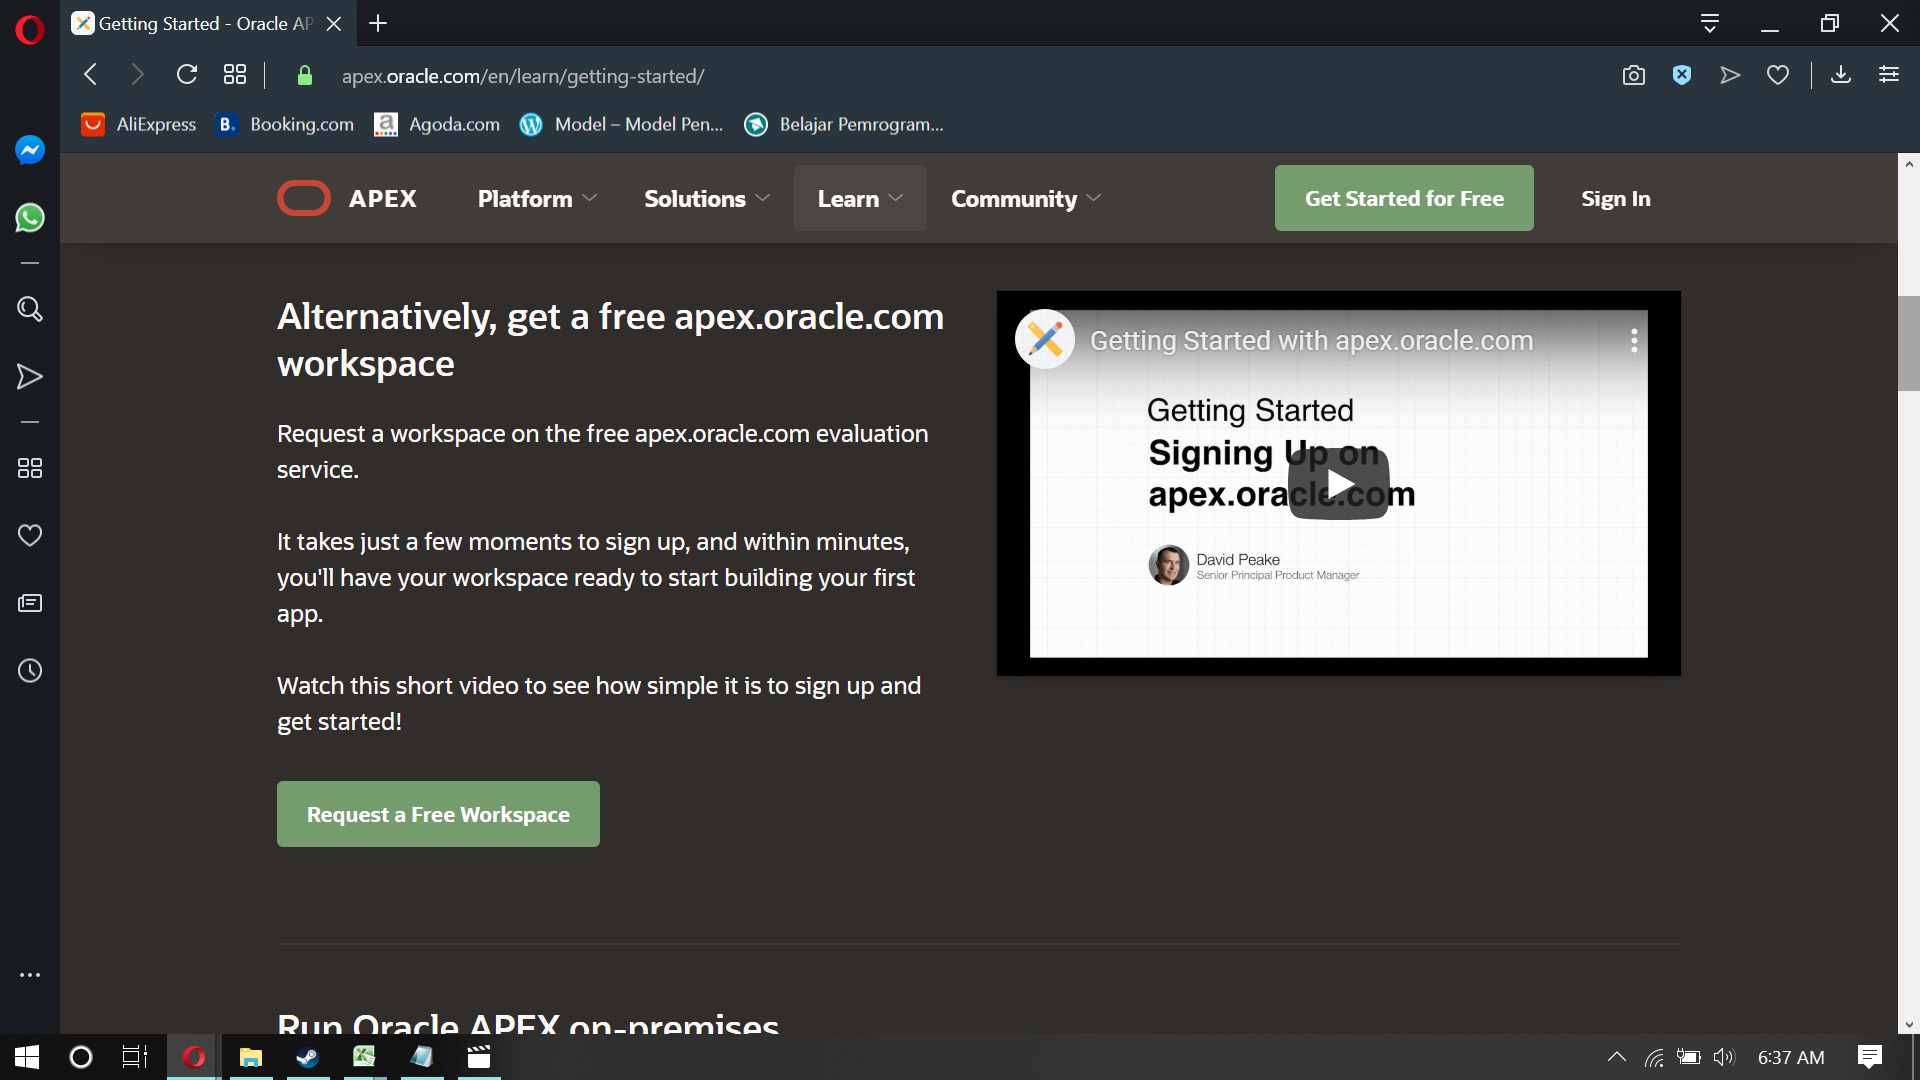
\includegraphics[width=10cm]{figures/gambar/Screenshot (106).png} 
    \caption{\textit{tampilan awal}}
    \label{foto1}
 	\end{figure}
	
	\item Isi form sesuai dengan yang dibutuhkan, lalu klik next.	
	
	\begin{figure}[H]
    \centering
    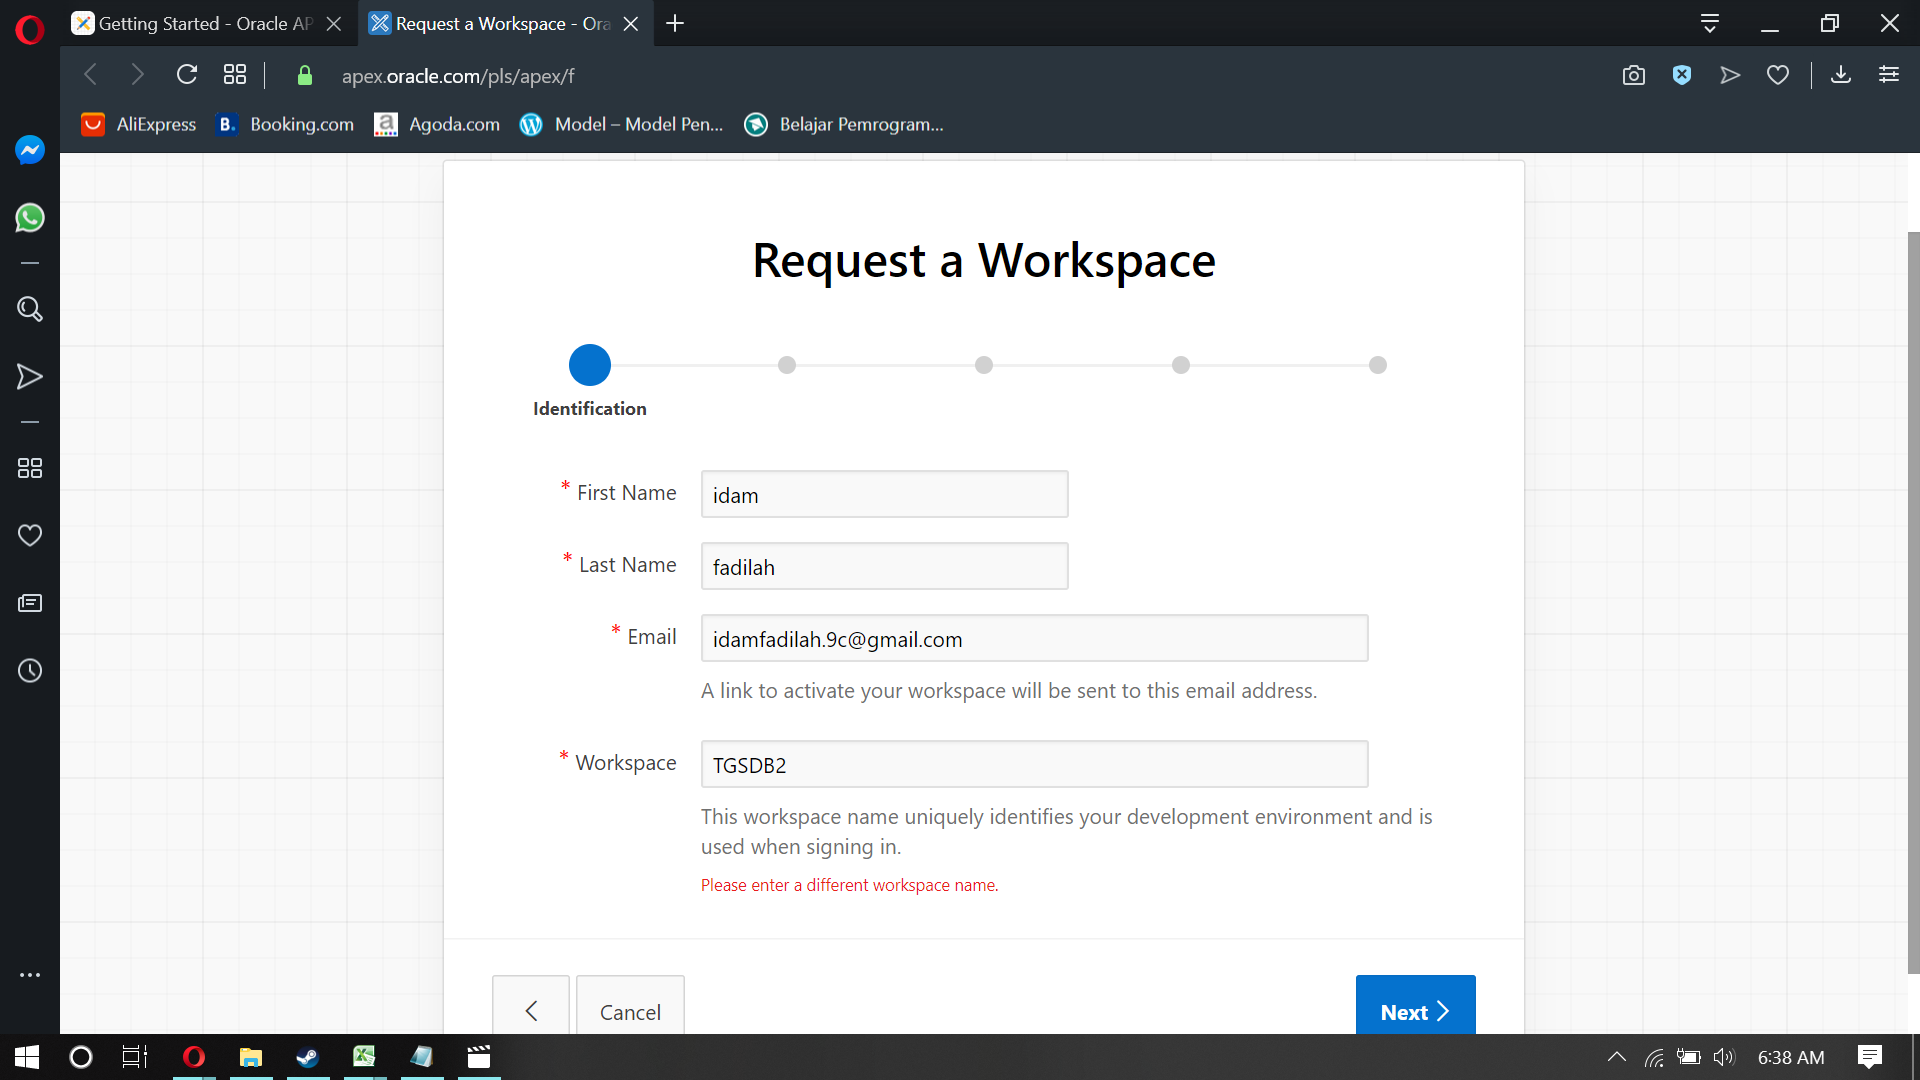
\includegraphics[width=10cm]{figures/gambar/Screenshot (108).png} 
    \caption{\textit{formulir request a workspace}}
    \label{foto2}
 	\end{figure}
	
	\item Cetang "yes" pada kedua penyataan, lalu klik next.
	
	\begin{figure}[H]
    \centering
    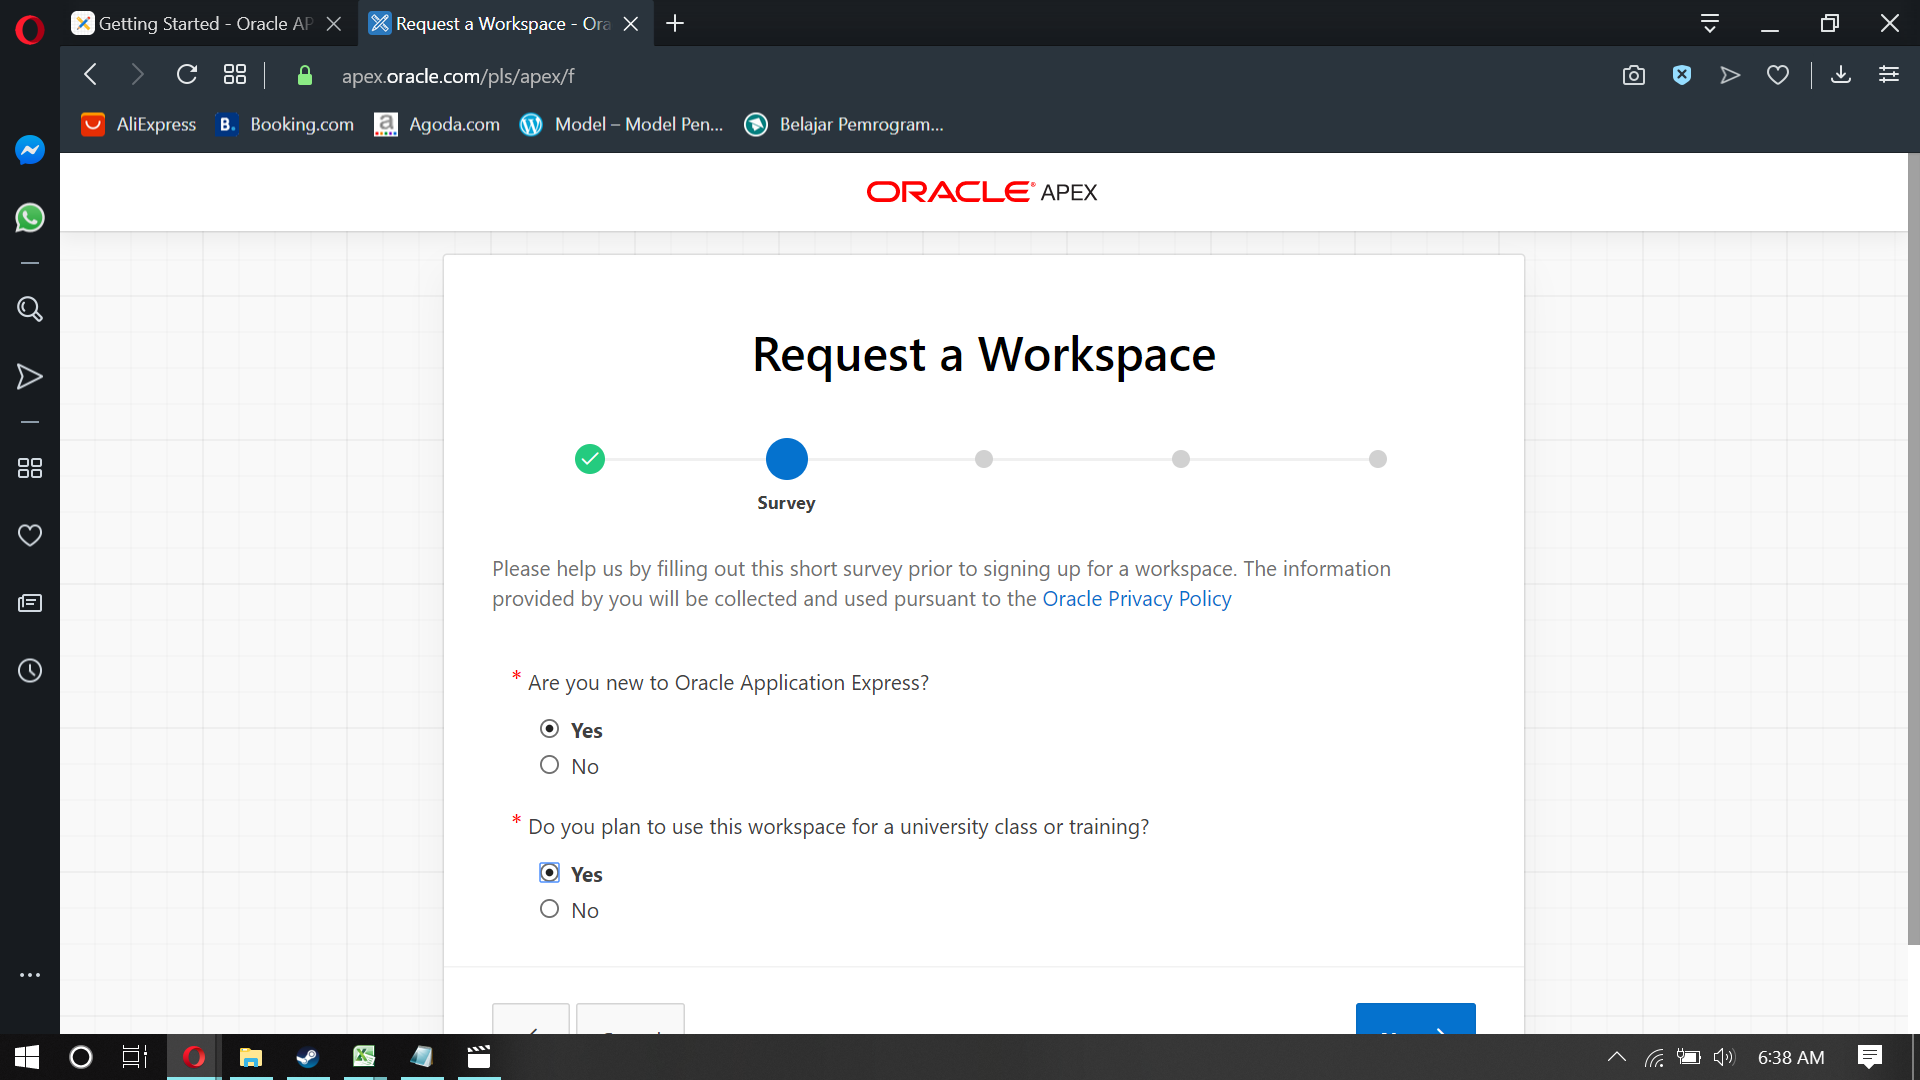
\includegraphics[width=10cm]{figures/gambar/Screenshot (109).png}  
    \caption{\textit{formulir request a workspace}}
    \label{foto3}
 	\end{figure}
		
	
	\item isi form sesuai kebutuhan, lalu klik next.	
	
	\begin{figure}[H]
    \centering
    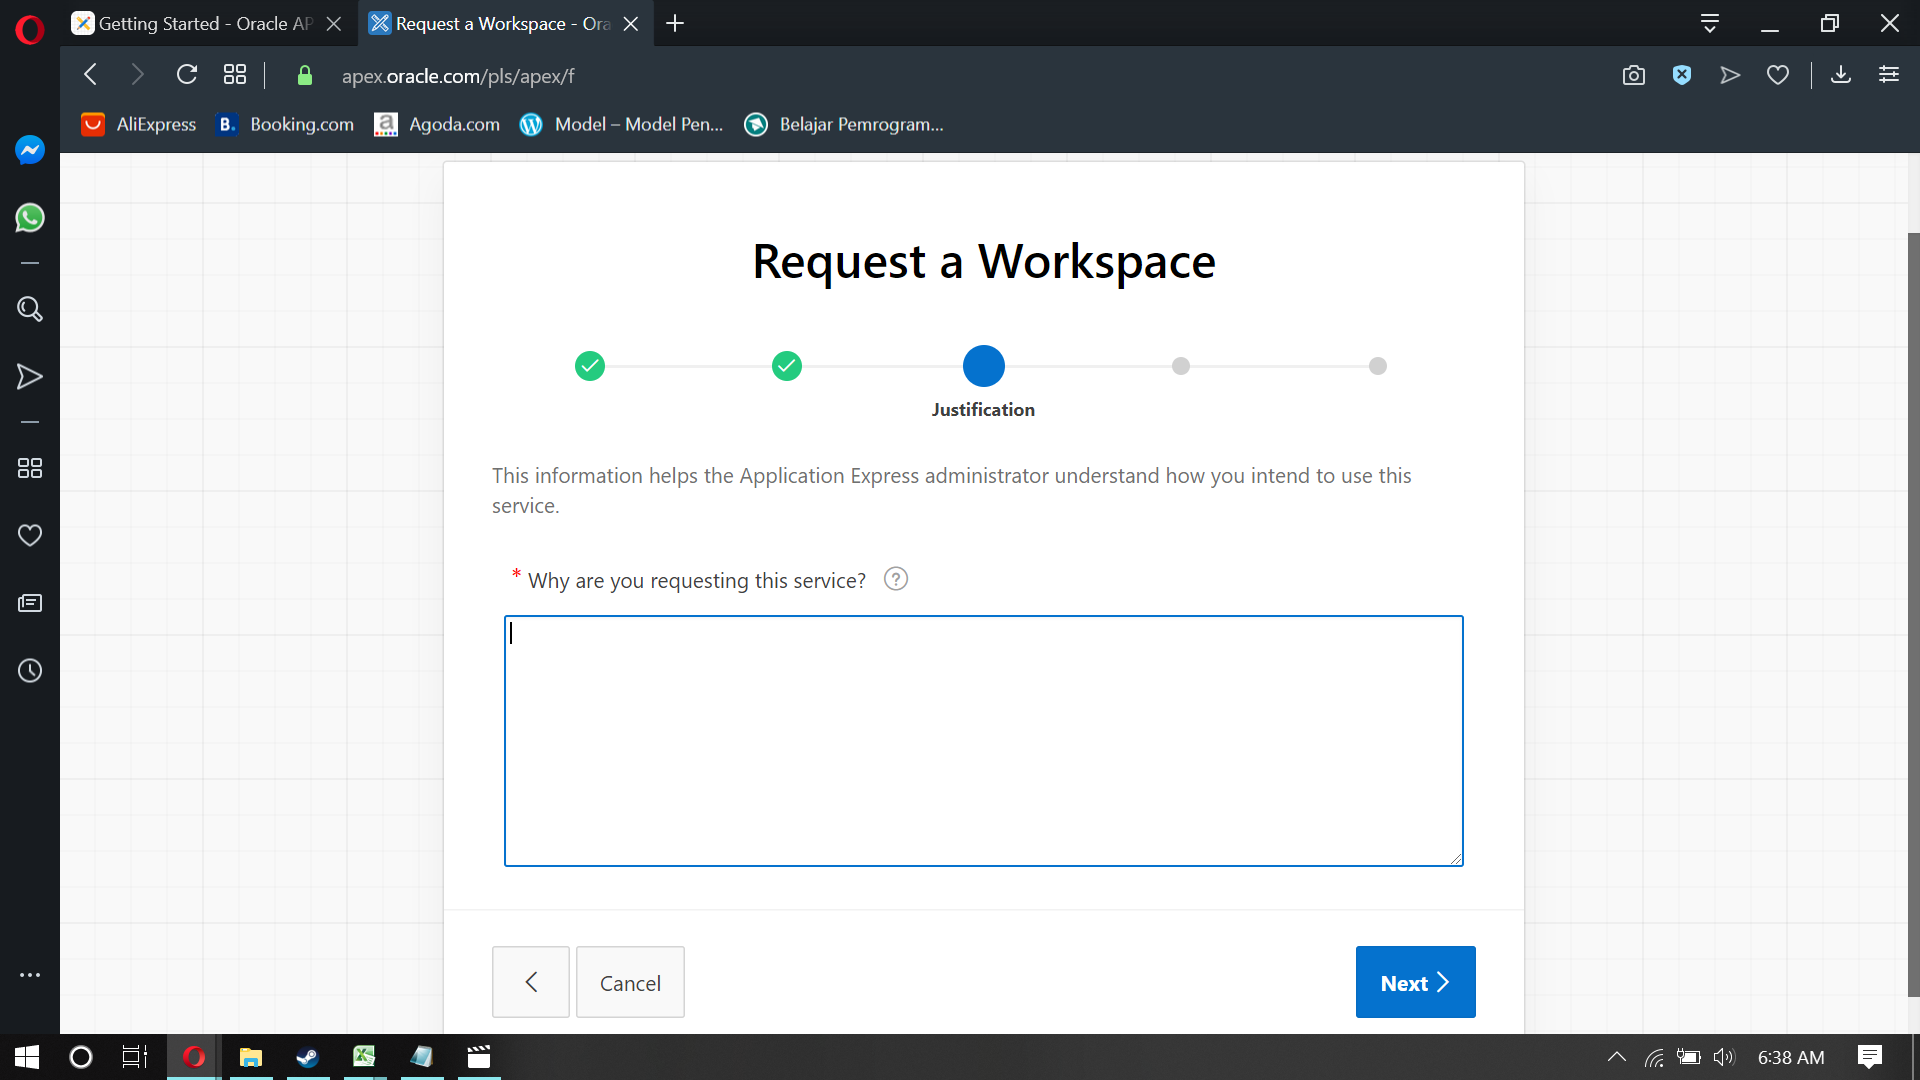
\includegraphics[width=10cm]{figures/gambar/Screenshot (110).png}  
    \caption{\textit{formulir request a workspace}}
    \label{foto4}
 	\end{figure}
	
	\item cetang accept, lalu klik next.
	
	\begin{figure}[H]
    \centering
    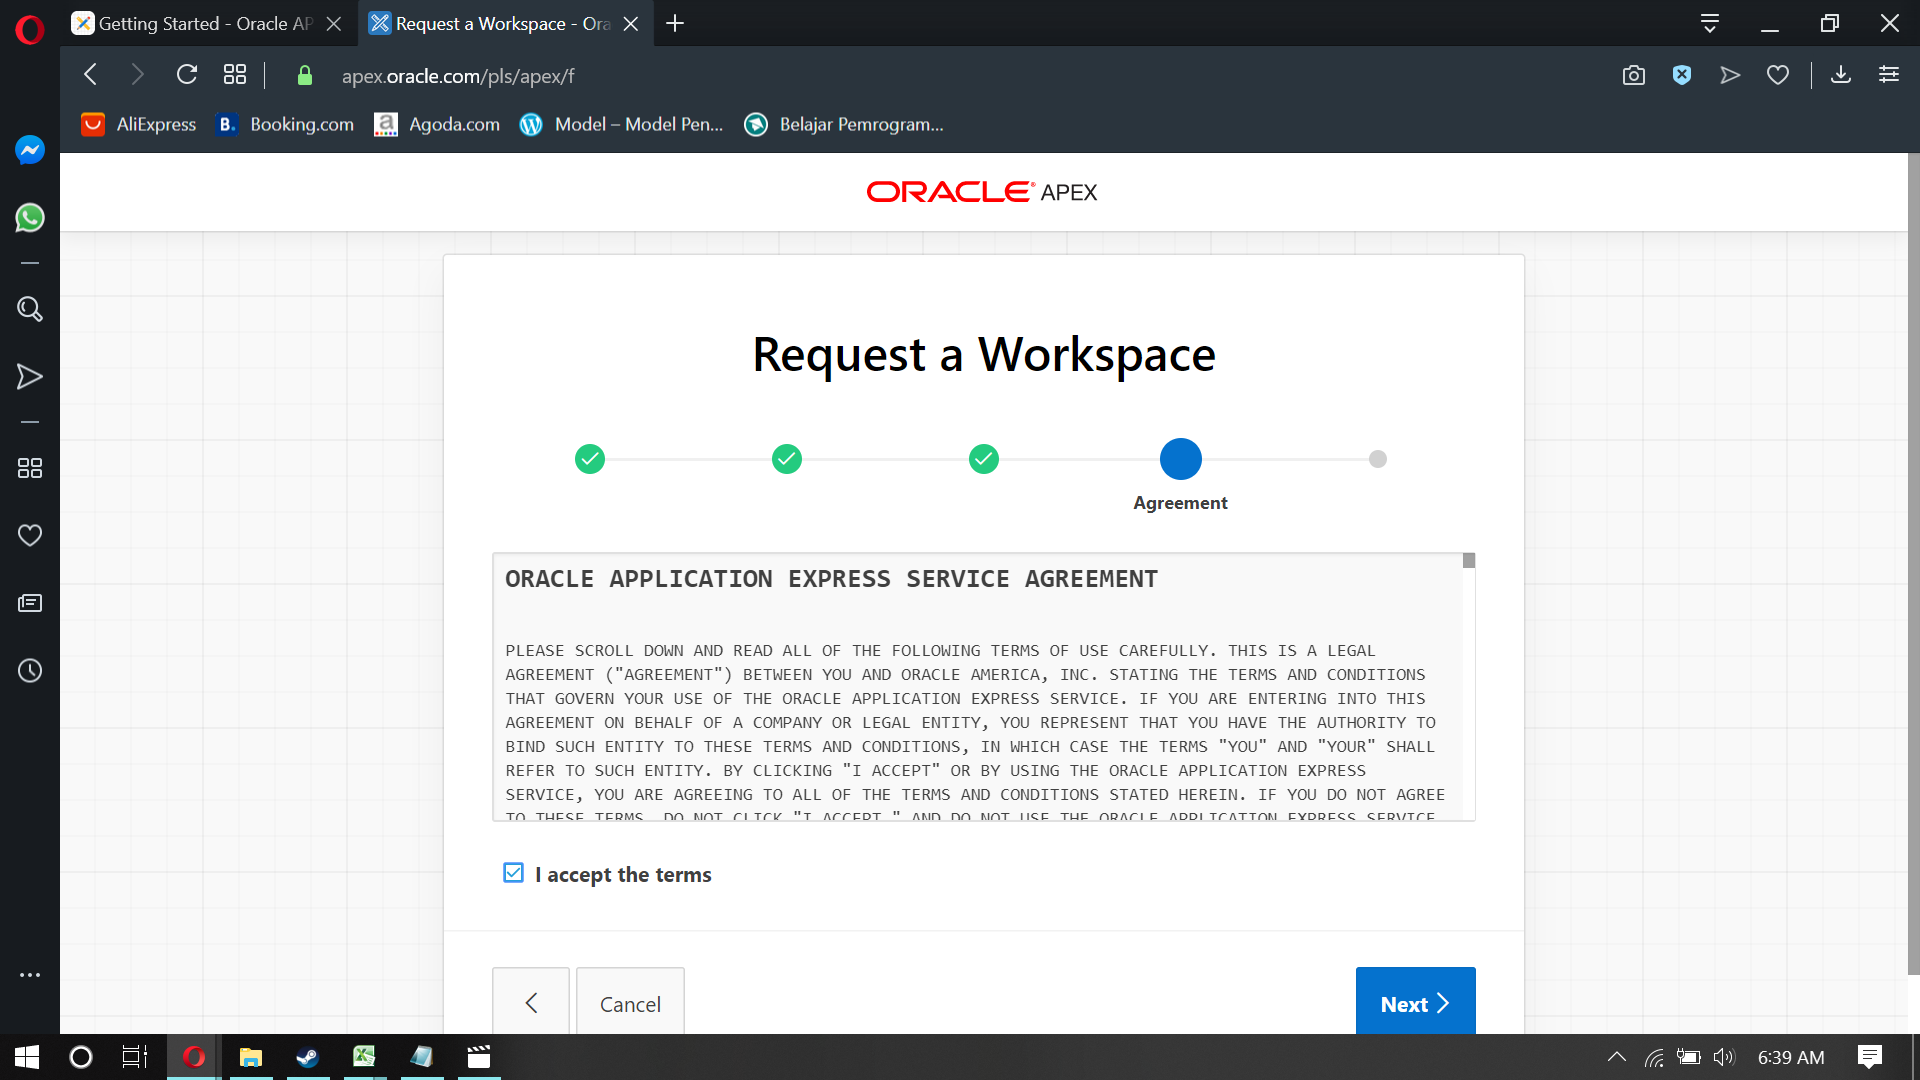
\includegraphics[width=10cm]{figures/gambar/Screenshot (111).png}  
    \caption{\textit{formulir request a workspace}}
    \label{foto5}
 	\end{figure}
 	
	\item klik submit request.
	
	\begin{figure}[H]
    \centering
    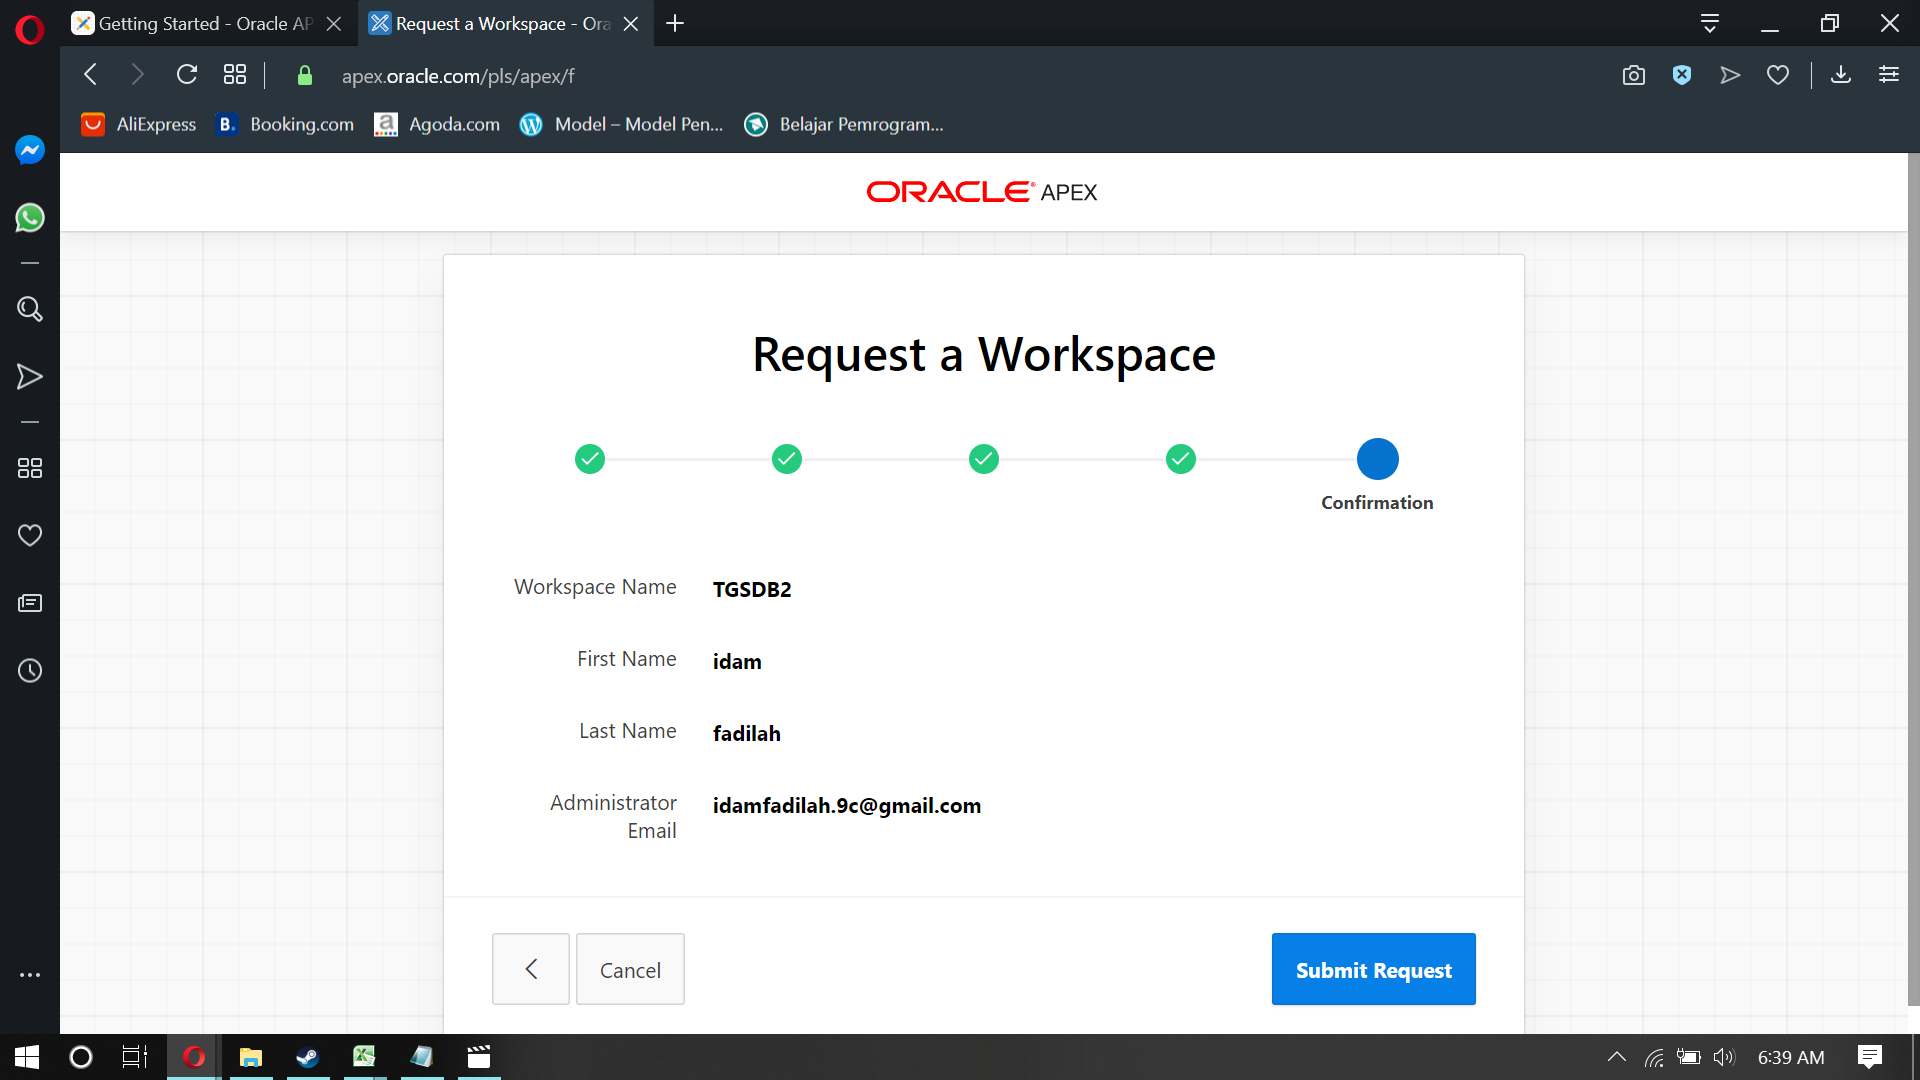
\includegraphics[width=10cm]{figures/gambar/Screenshot (112).png} 
    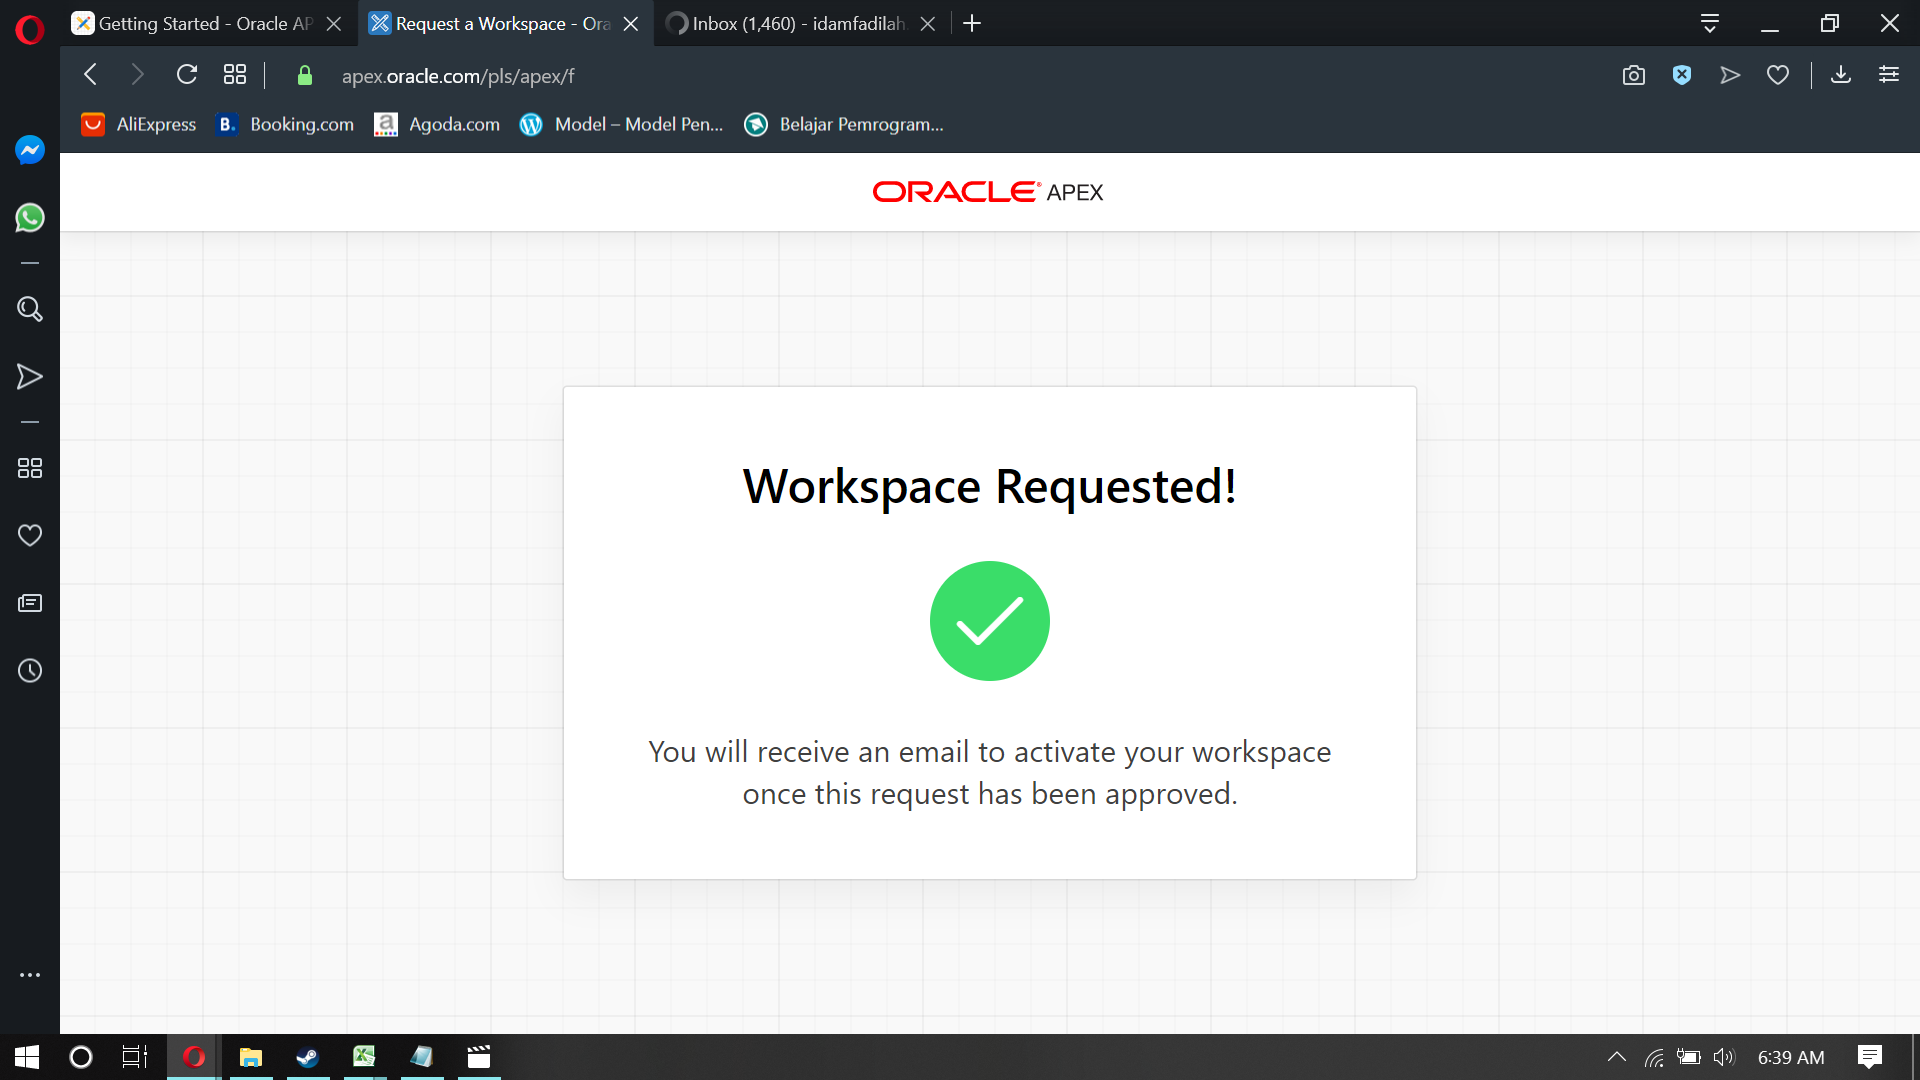
\includegraphics[width=10cm]{figures/gambar/Screenshot (113).png}  
    \caption{\textit{formulir request a workspace}}
    \label{foto6}
 	\end{figure}	
	
	\item buka email dari oracle lalu klik create workspace.
	
	\begin{figure}[H]
    \centering
    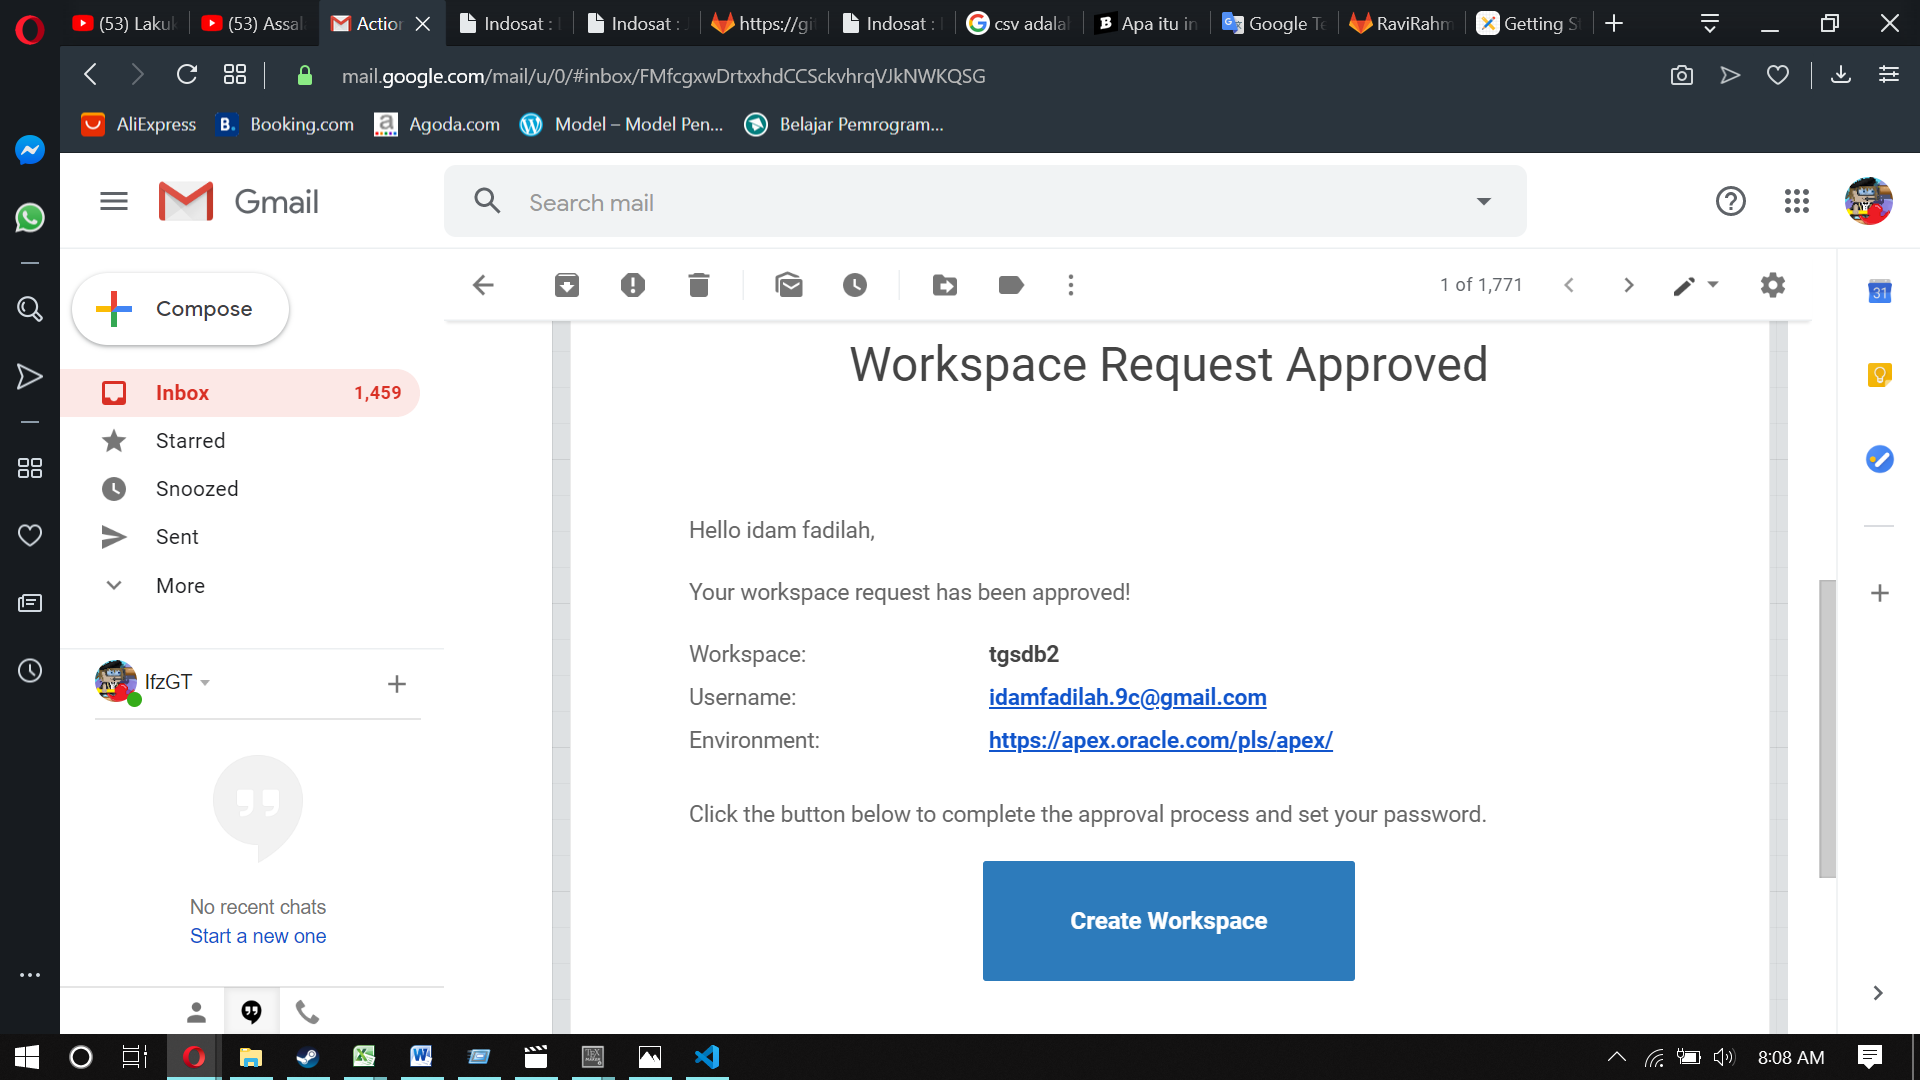
\includegraphics[width=10cm]{figures/gambar/Screenshot (119).png}  
    \caption{\textit{request workspace approve}}
    \label{foto7}
 	\end{figure}
 	
	\item lalu login ke Oracle APEX, dengan data yang sudah didaftarkan.
	
	\begin{figure}[H]
    \centering
    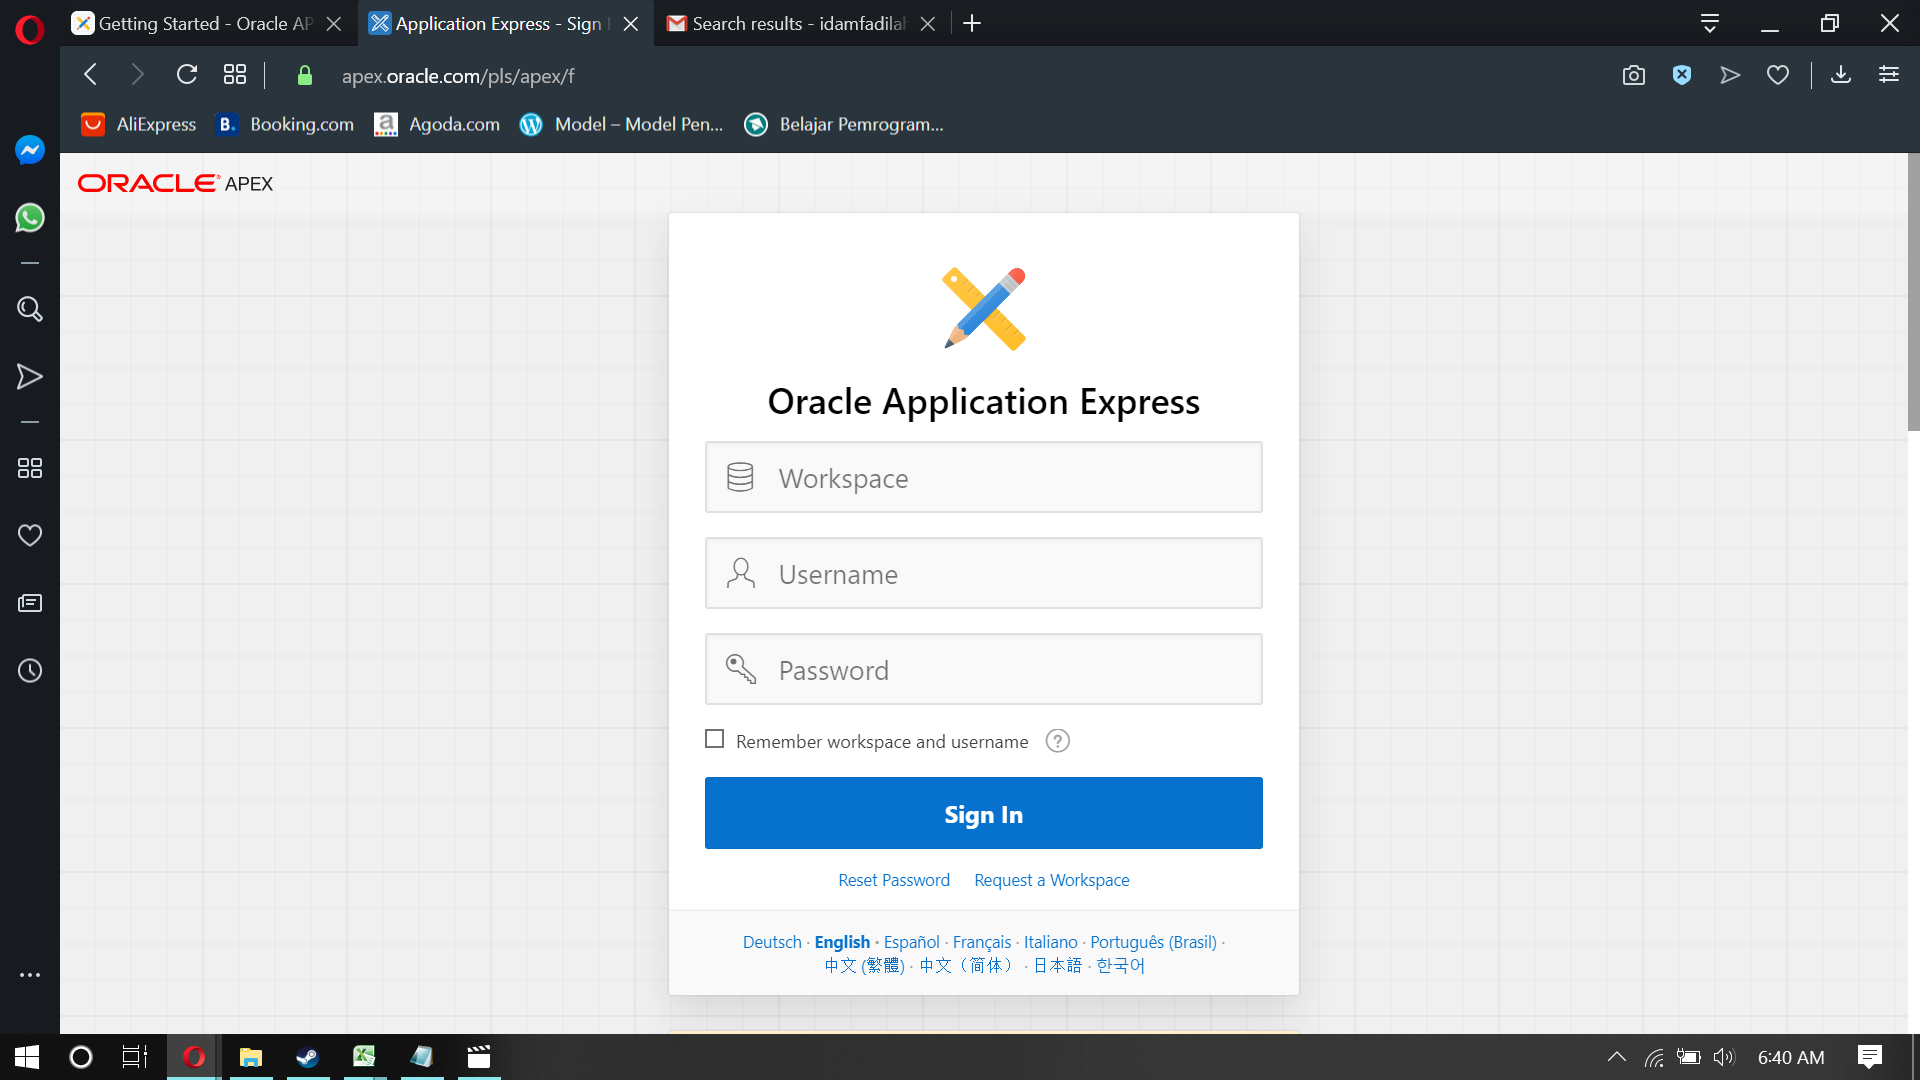
\includegraphics[width=10cm]{figures/gambar/Screenshot (114).png}  
    \caption{\textit{login apex}}
    \label{foto8}
 	\end{figure}
 	
	\item tampilan sesudah login, selesai.
	
	\begin{figure}[H]
    \centering
    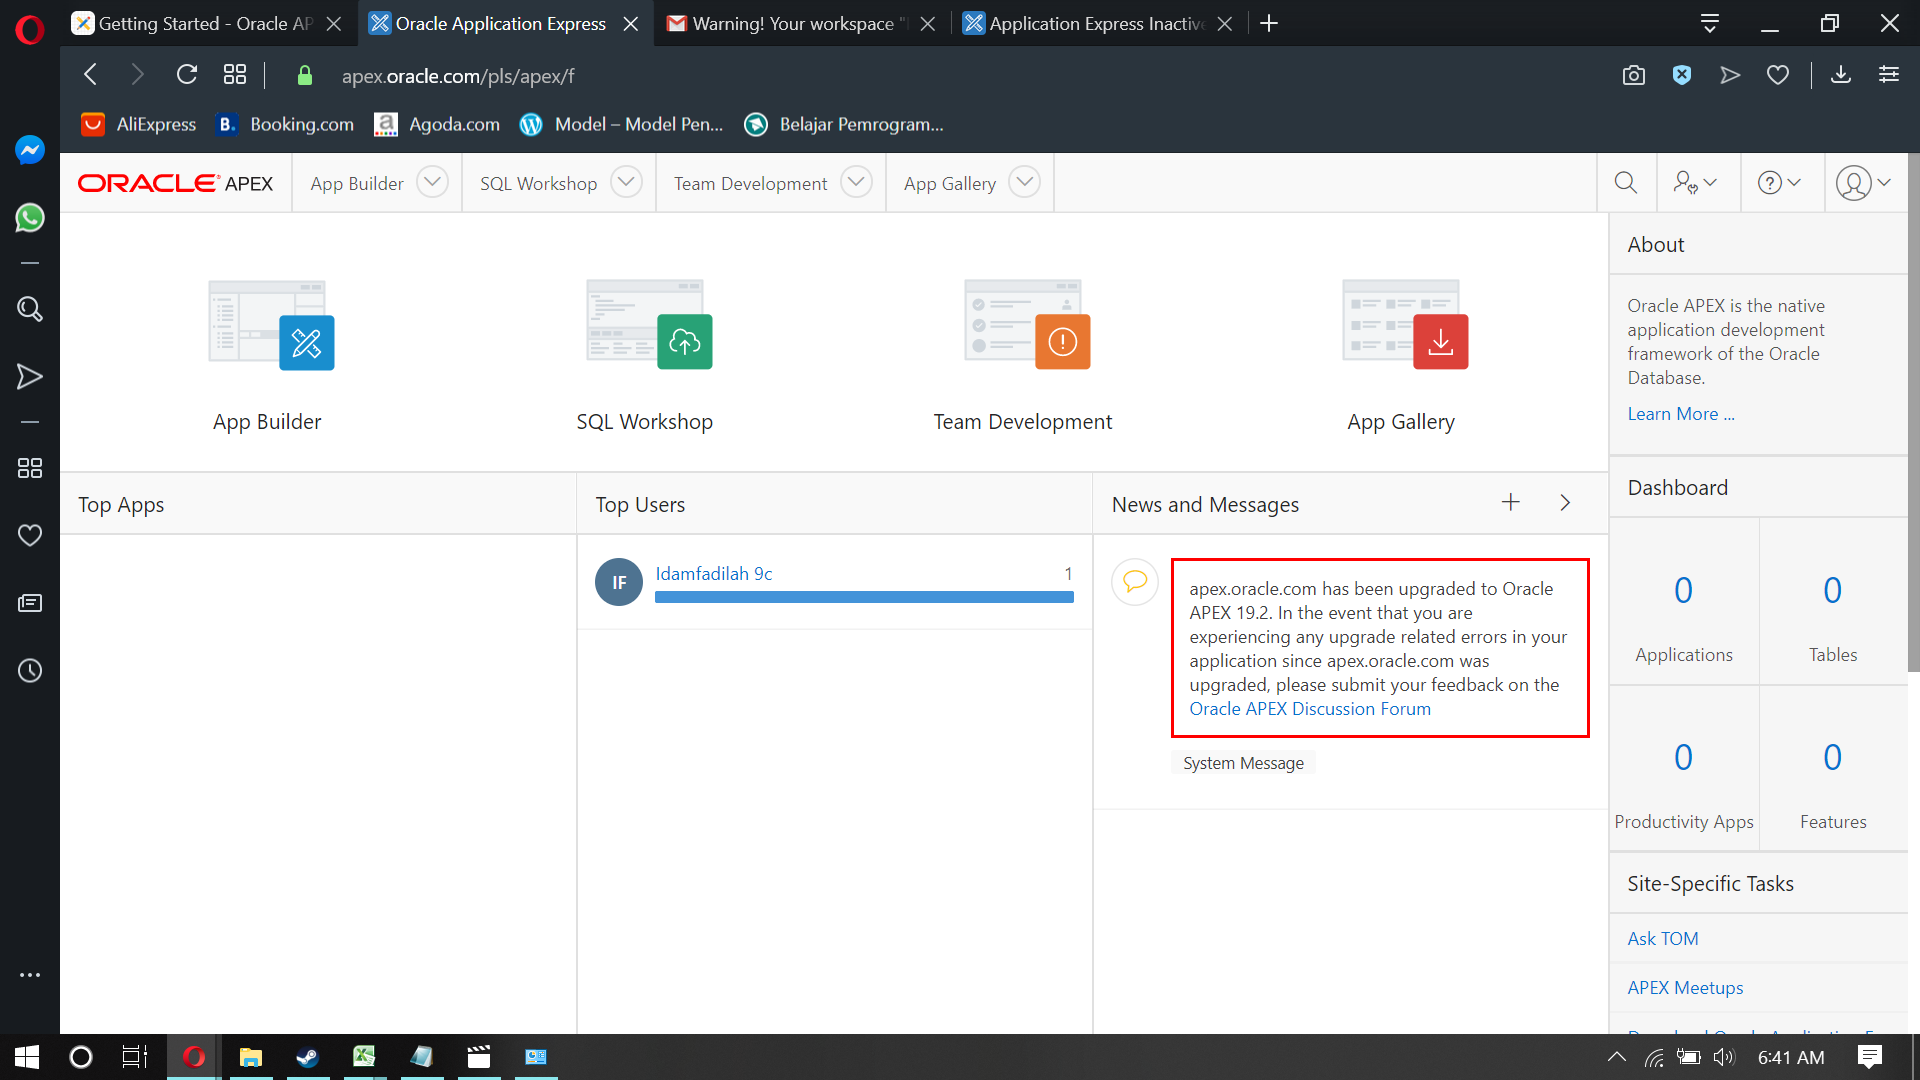
\includegraphics[width=10cm]{figures/gambar/Screenshot (115).png}  
    \caption{\textit{menu home apex}}
    \label{foto9}
 	\end{figure}
 	
\end{enumerate}
\section{import table dari file excel}
\paragraph{}
\begin{enumerate}
	\item siapkan terlebih dahulu data excel yang akan di import, disini saya menggunakan contoh data akademik, dengan 5 dokumen excel yaitu mahasiswa, dosen, matakuliah, jadwal, dan nilai. jika ingin mendownload contoh data yang saya pakai bisa kunjungi \url{https://bit.ly/2QhvWSs}.
	\begin{figure}[H]
    \centering
    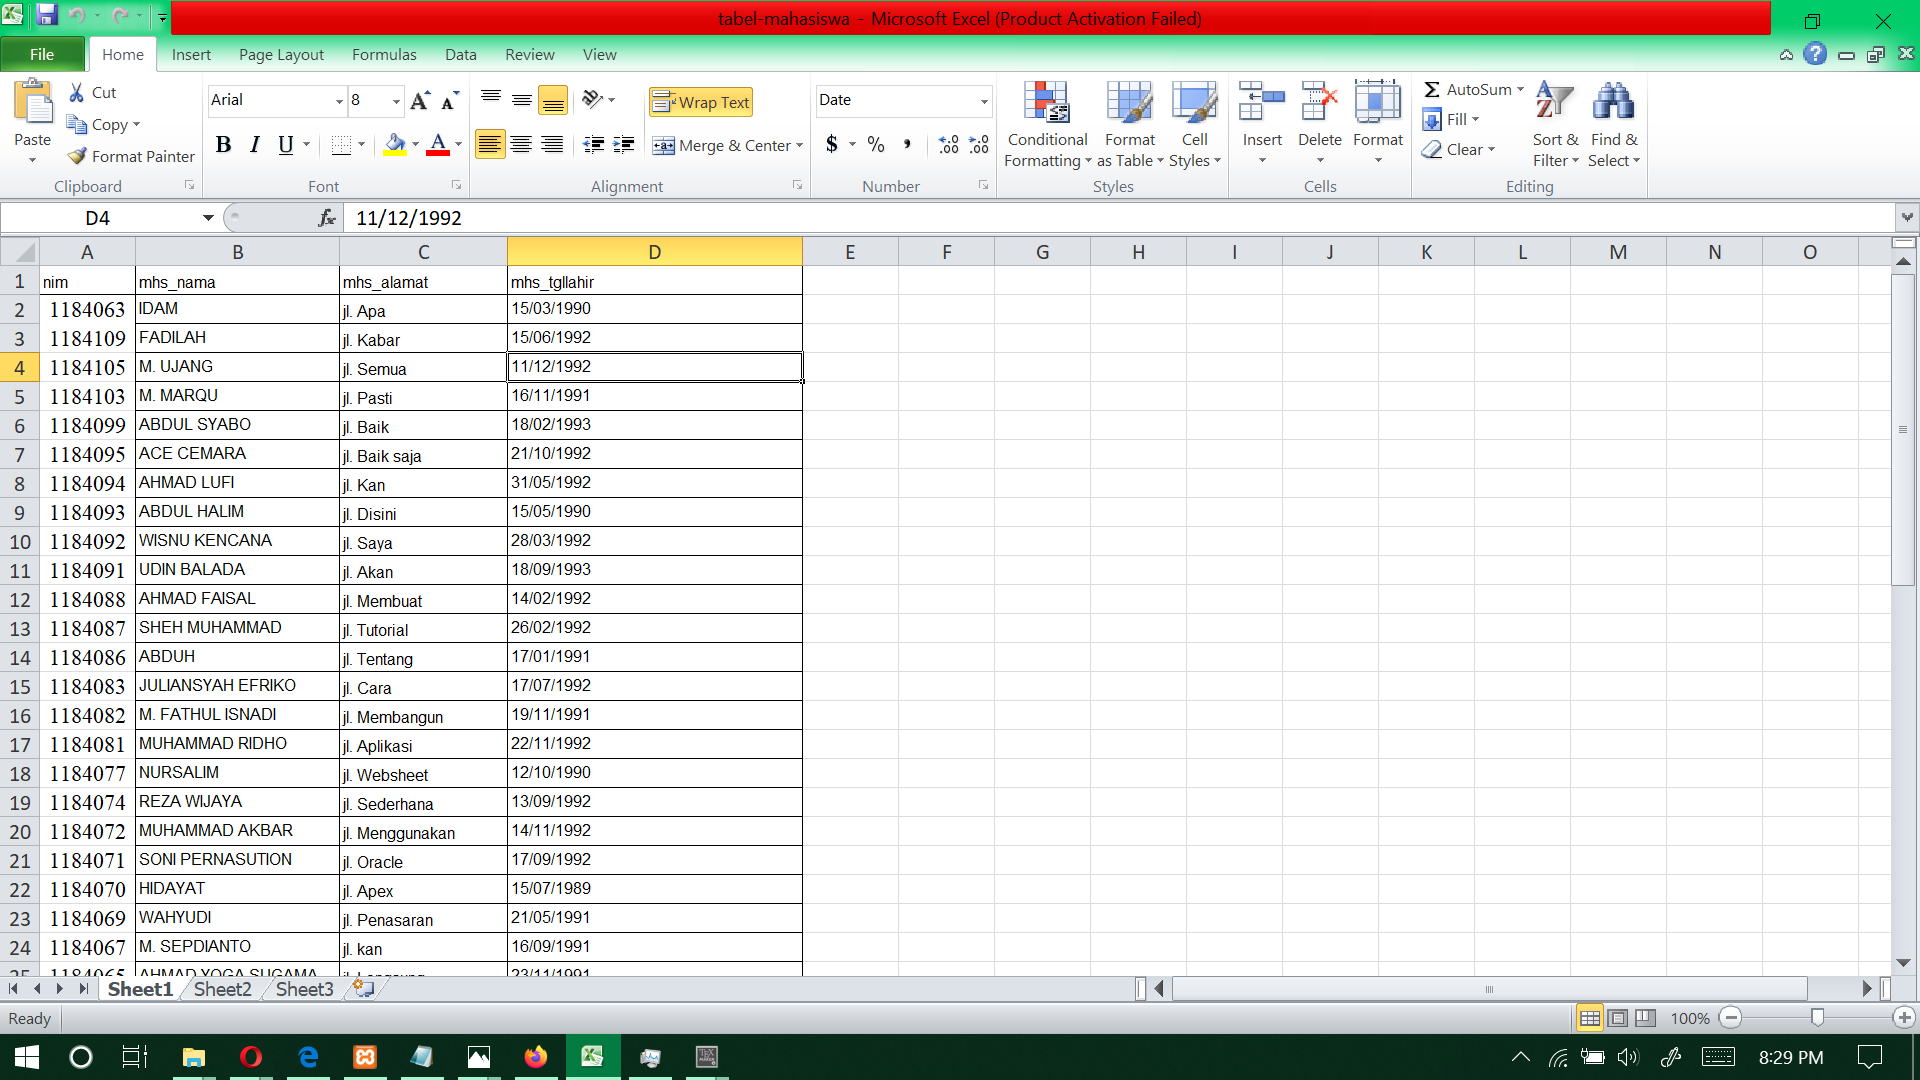
\includegraphics[width=10cm]{figures/persiapan data/Screenshot (224).png}
    \caption{\textit{data mahasiswa}}
    \label{foto10}
 	\end{figure}
 	\begin{figure}[H]
    \centering
    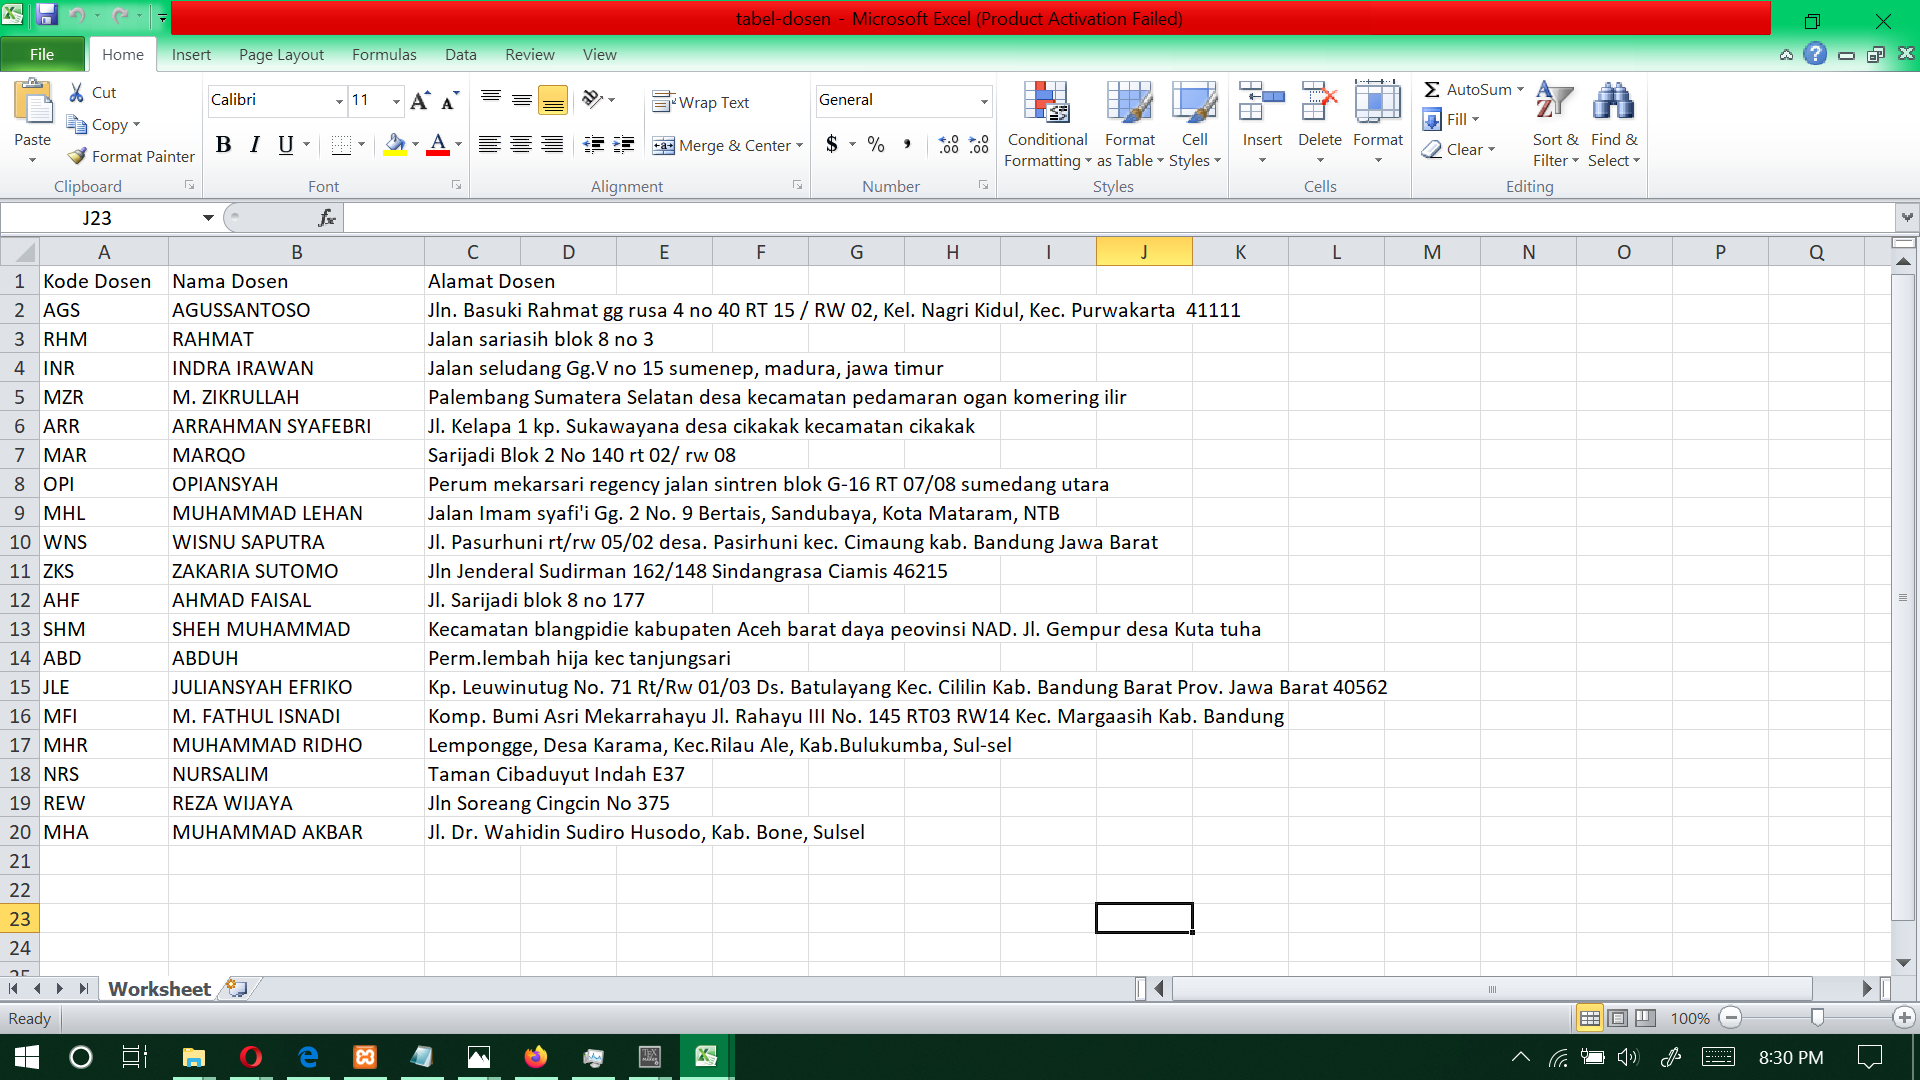
\includegraphics[width=10cm]{figures/persiapan data/Screenshot (225).png} 
    \caption{\textit{data dosen}}
    \label{foto11}
 	\end{figure}
 	\begin{figure}[H]
    \centering
    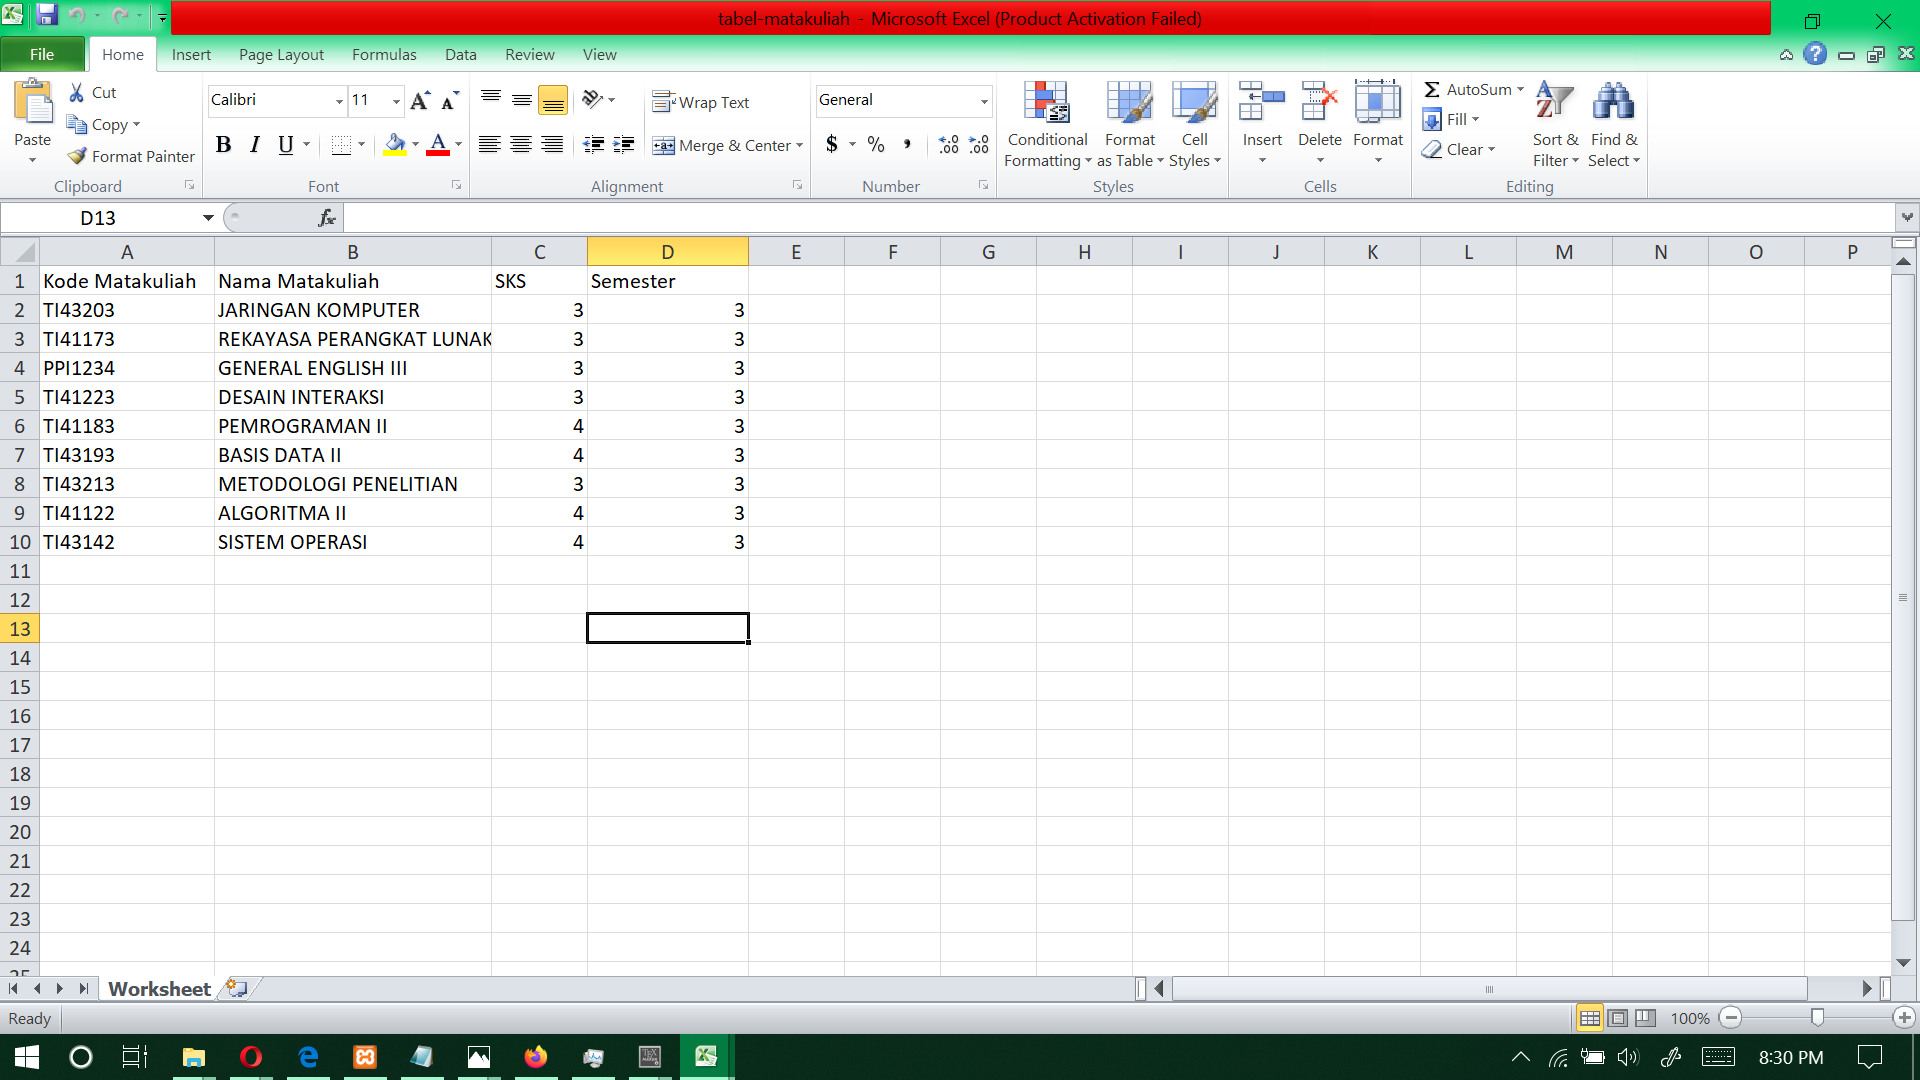
\includegraphics[width=10cm]{figures/persiapan data/Screenshot (226).png}
    \caption{\textit{data matakuliah}}
    \label{foto12}
 	\end{figure}
 	\begin{figure}[H]
    \centering
    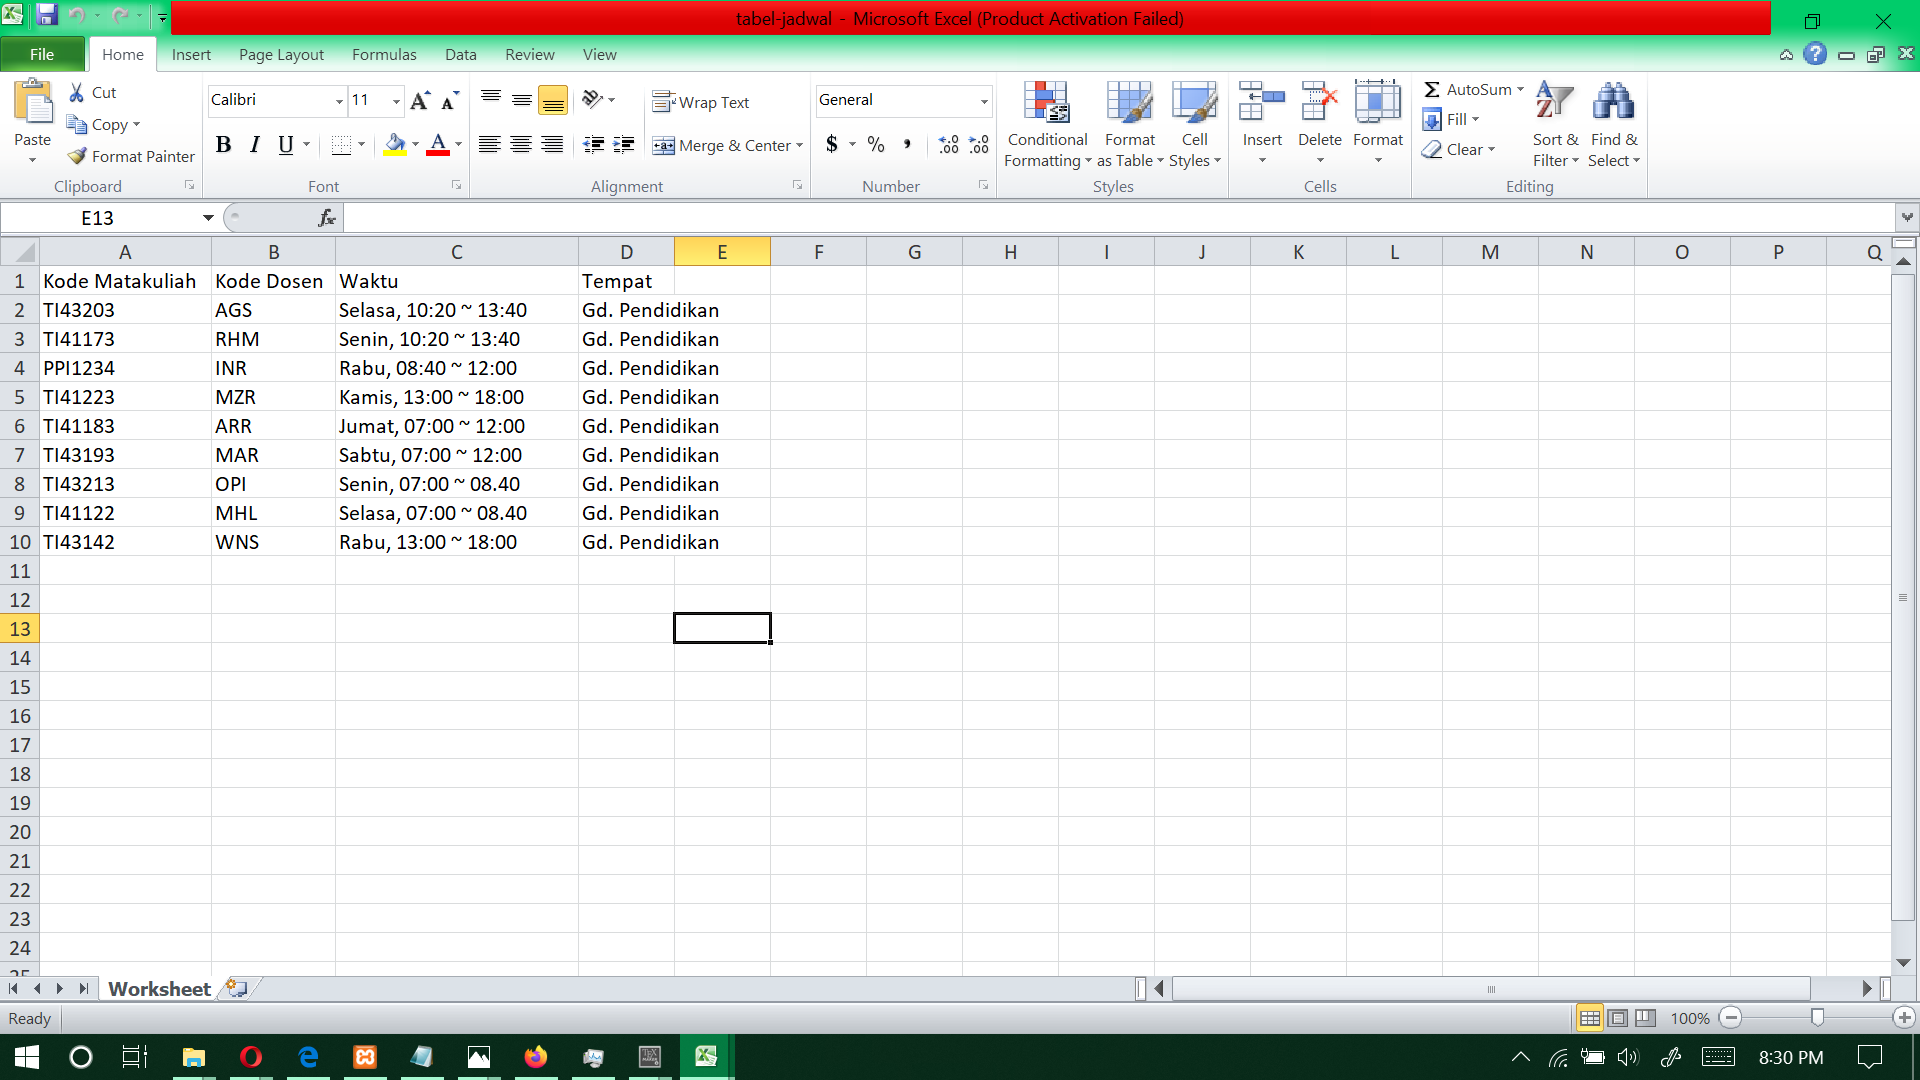
\includegraphics[width=10cm]{figures/persiapan data/Screenshot (227).png}
    \caption{\textit{data jadwal}}
    \label{foto13}
 	\end{figure}
 	\begin{figure}[H]
    \centering
    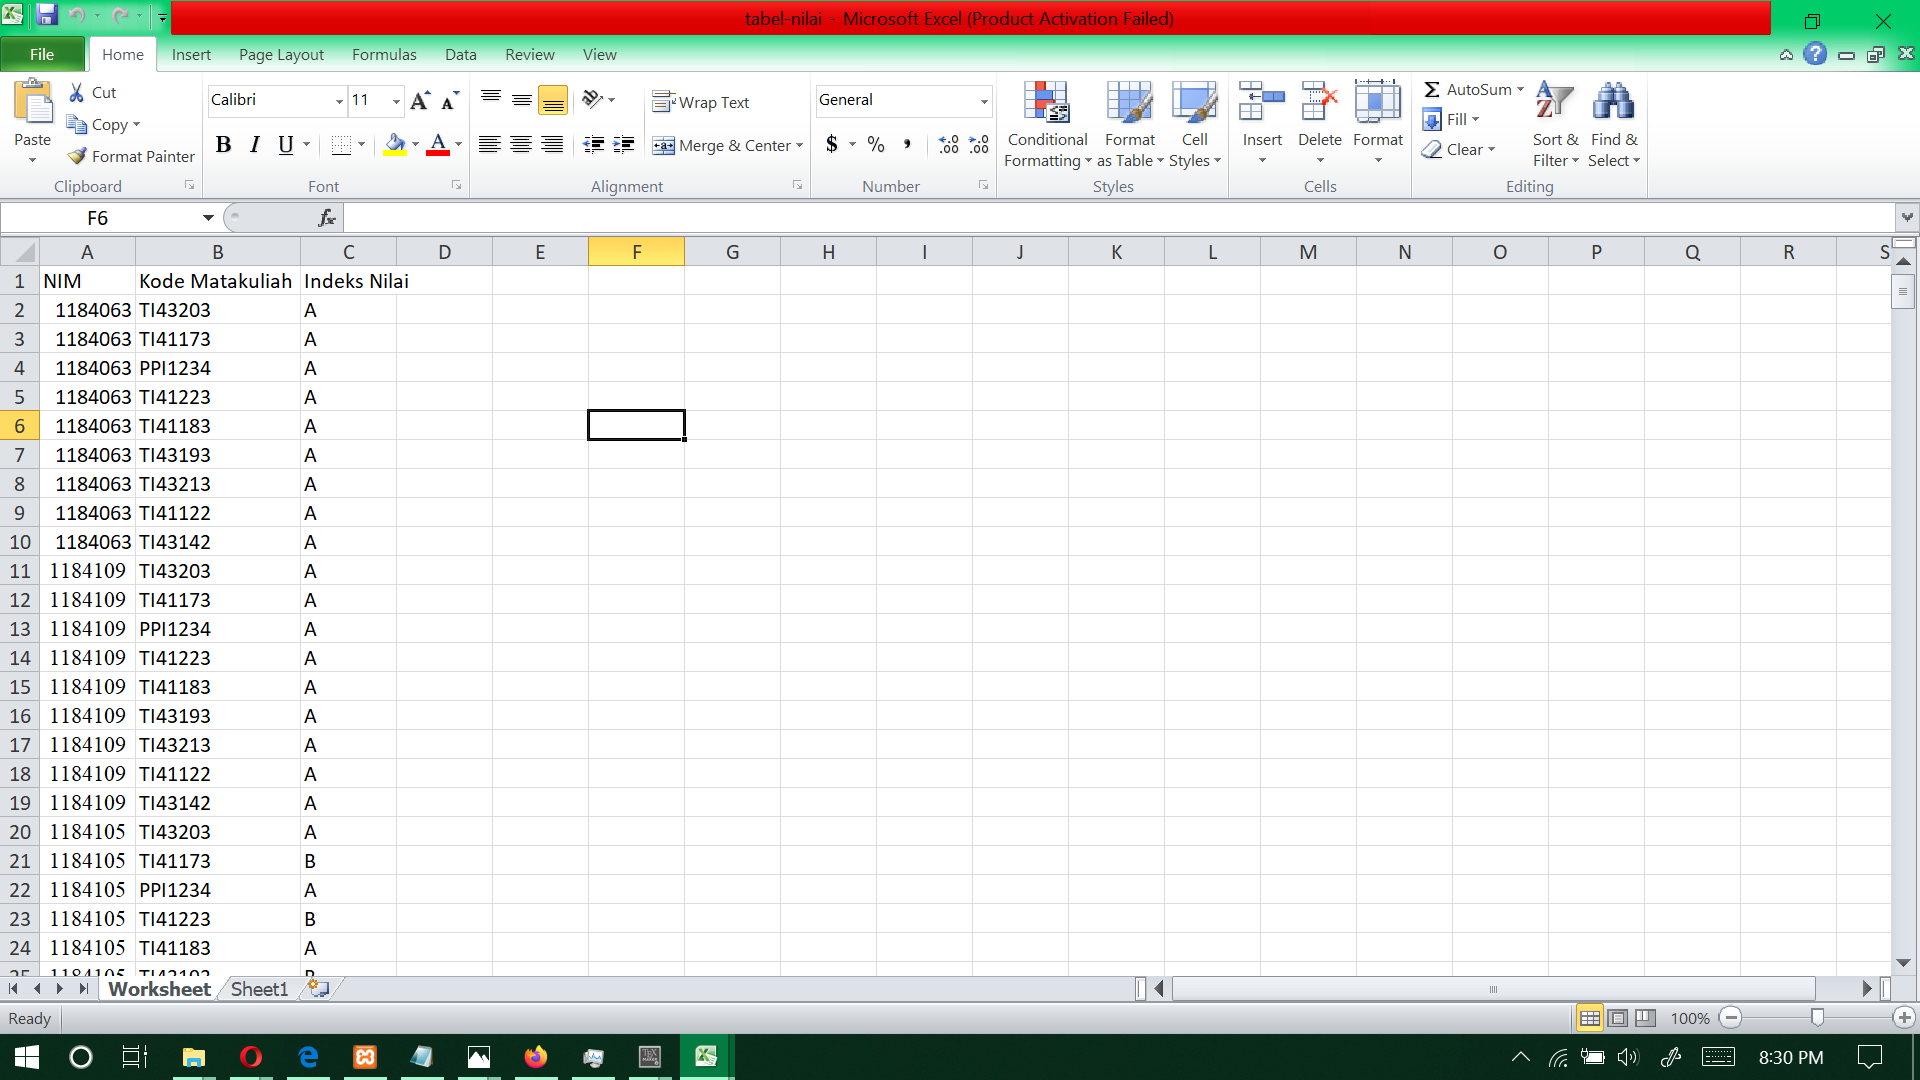
\includegraphics[width=10cm]{figures/persiapan data/Screenshot (228).png}
    \caption{\textit{data nilai}}
    \label{foto14}
 	\end{figure}
	\item perhatikan pada dokumen excel kolom pertama pada dokumen akan menjadi nama kolom pada tabel database nantinya, contoh pada dokumen tabel-mahasiswa pada kolom pertama setiap baris terdapat nim,mhs\_nama,mhs\_alamat,dan mhs\_tgllahir.
	\begin{figure}[H]
    \centering
	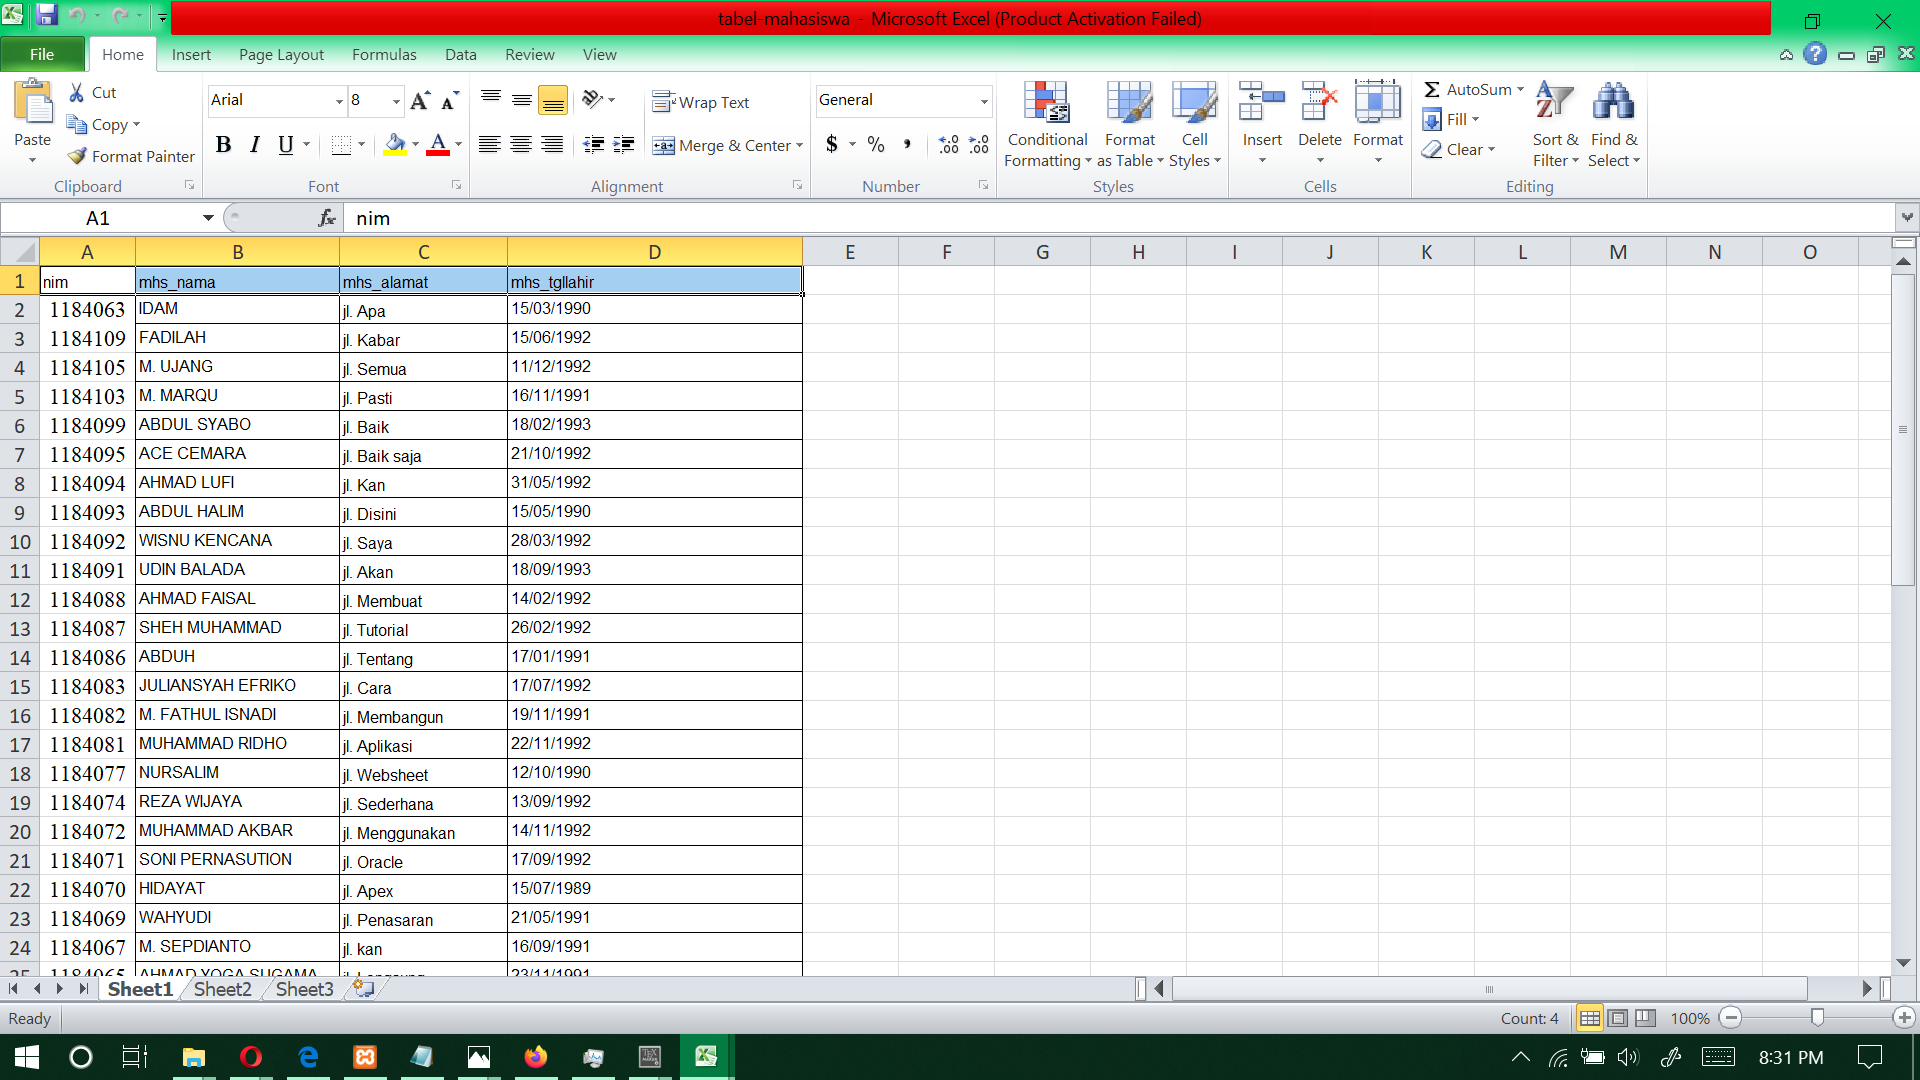
\includegraphics[width=10cm]{figures/persiapan data/Screenshot (229).png} 
    \caption{\textit{data mahasiswa}}
    \label{foto15}
 	\end{figure}
	\item kemudian jika semua data sudah disiapkan, maka langkah selanjutnya yaitu mengimport file excel ke apex, klik dropdown pada bagian "SQL workshop" lalu "utilities" pilih "Data Workshop".
	\begin{figure}[H]
    \centering
	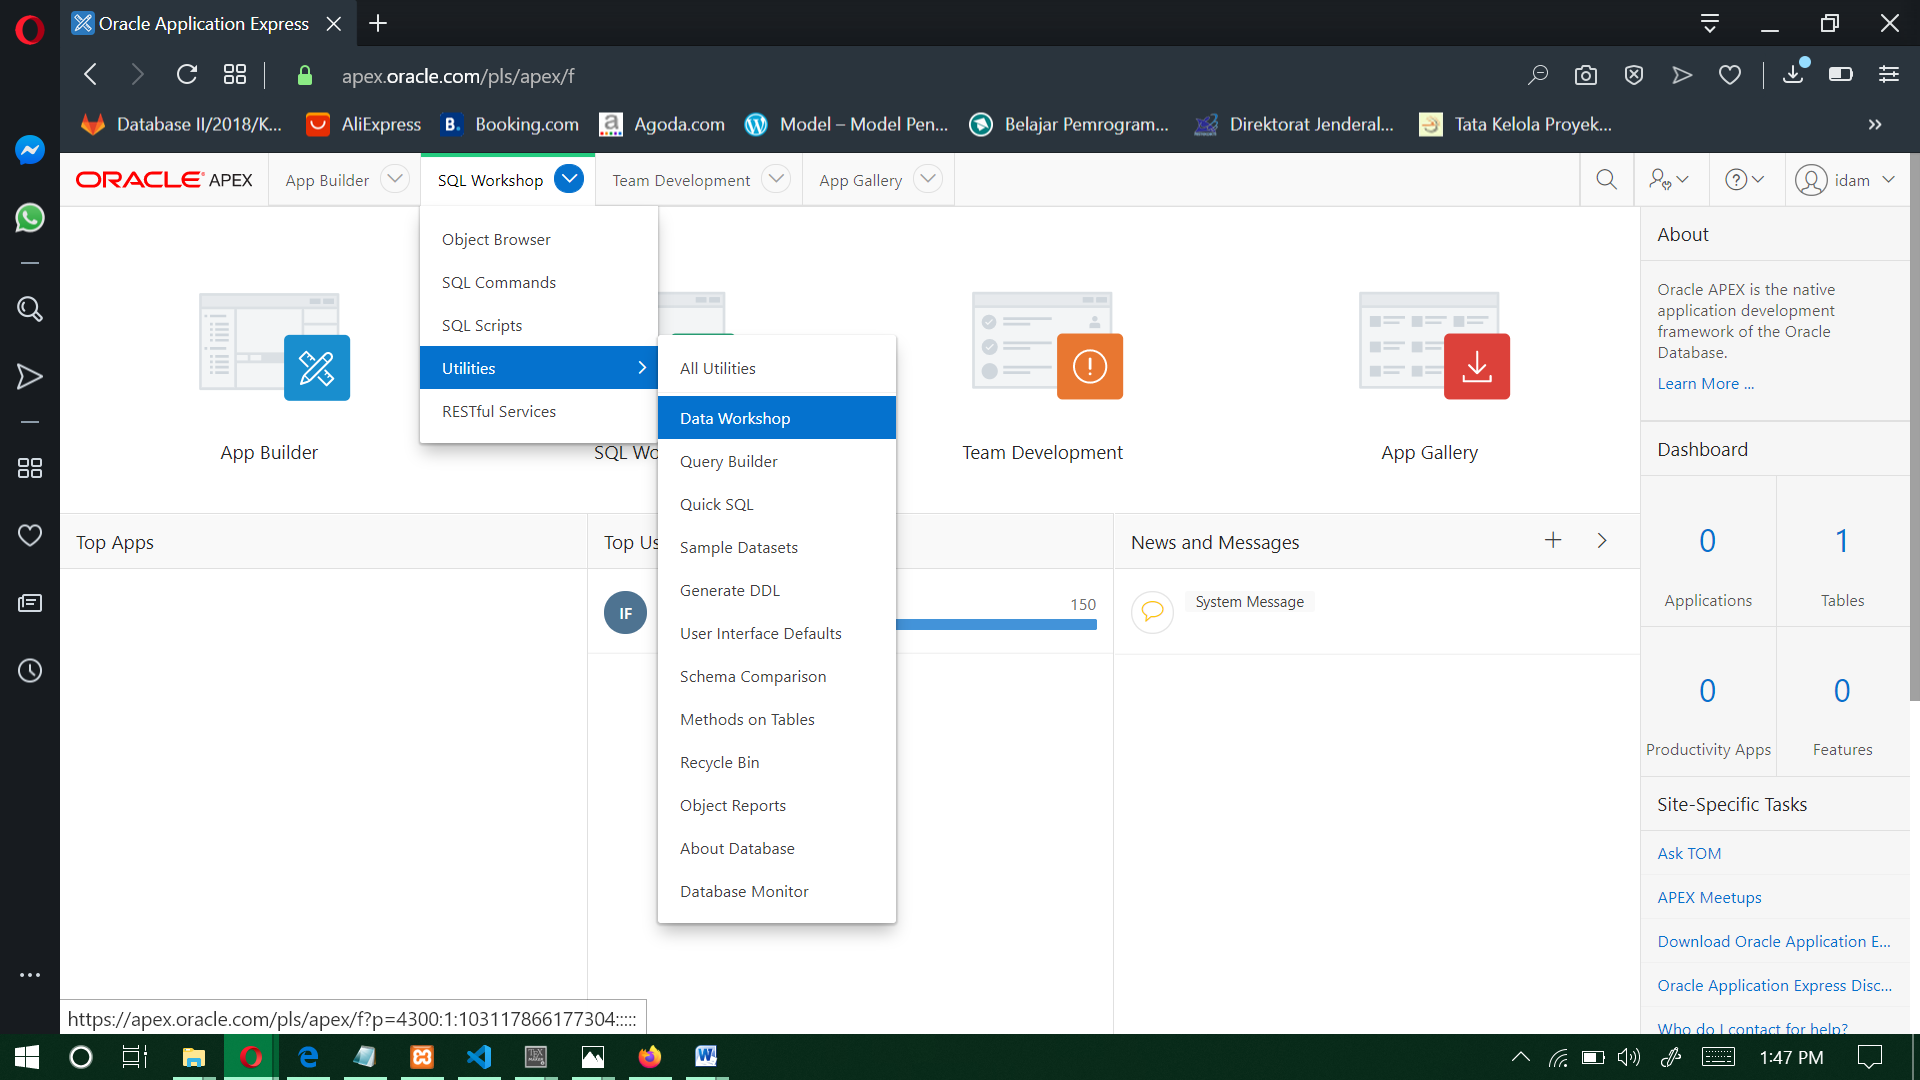
\includegraphics[width=10cm]{figures/load data csv/Screenshot (207).png} 
    \caption{\textit{oracle apex - home}}
    \label{foto16}
 	\end{figure}
	\item lalu klik "Load Data", lalu pilih file excel yang akan di import, contoh disini saya import file "tabel-mahasiswa", jika sudah dipilih maka klik open.
	\begin{figure}[H]
    \centering
	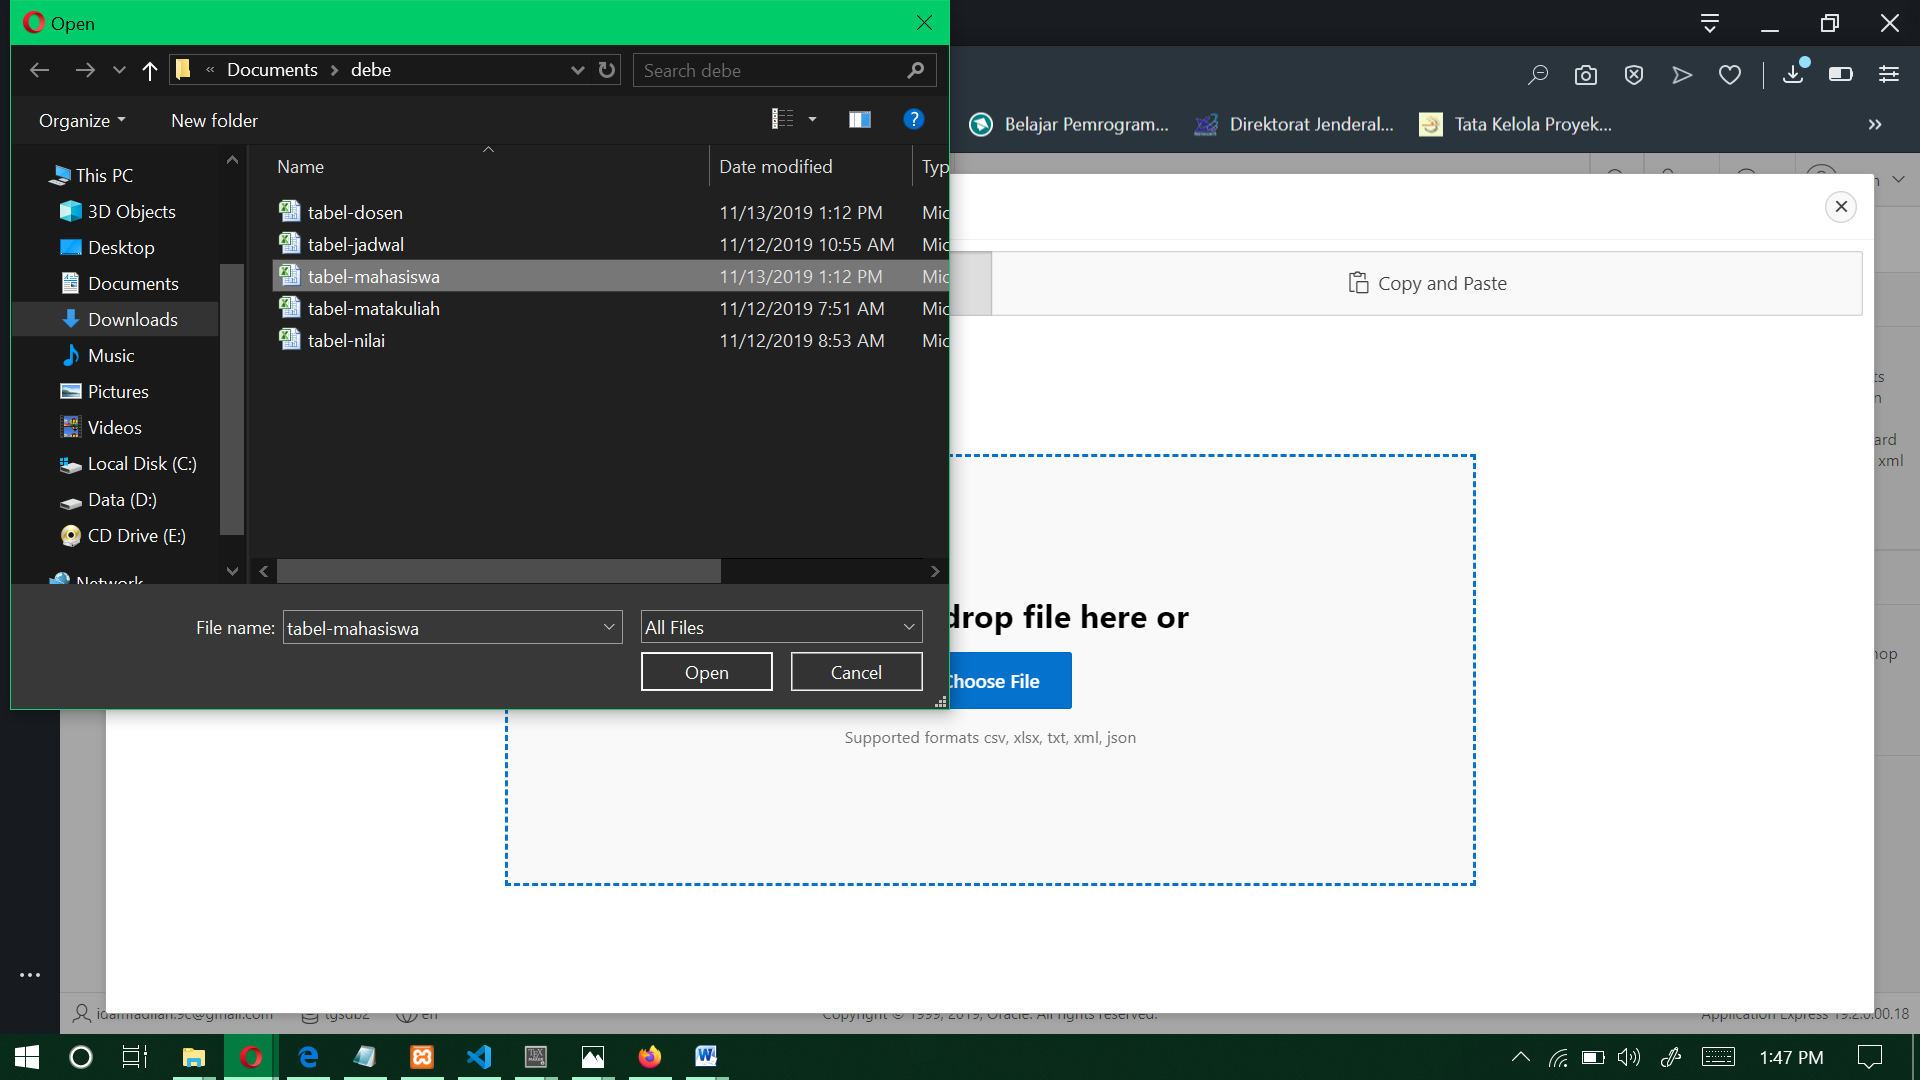
\includegraphics[width=10cm]{figures/load data csv/Screenshot (210).png} 
    \caption{\textit{load data excel}}
    \label{foto17}
 	\end{figure}
	\item jika sudah open file  maka akan muncul tampilan seperti dibawah ini, isi bagian Table name, jika sudah maka akan muncul tulisan "please select the columns to load" klik configure.
	\begin{figure}[H]
    \centering
	 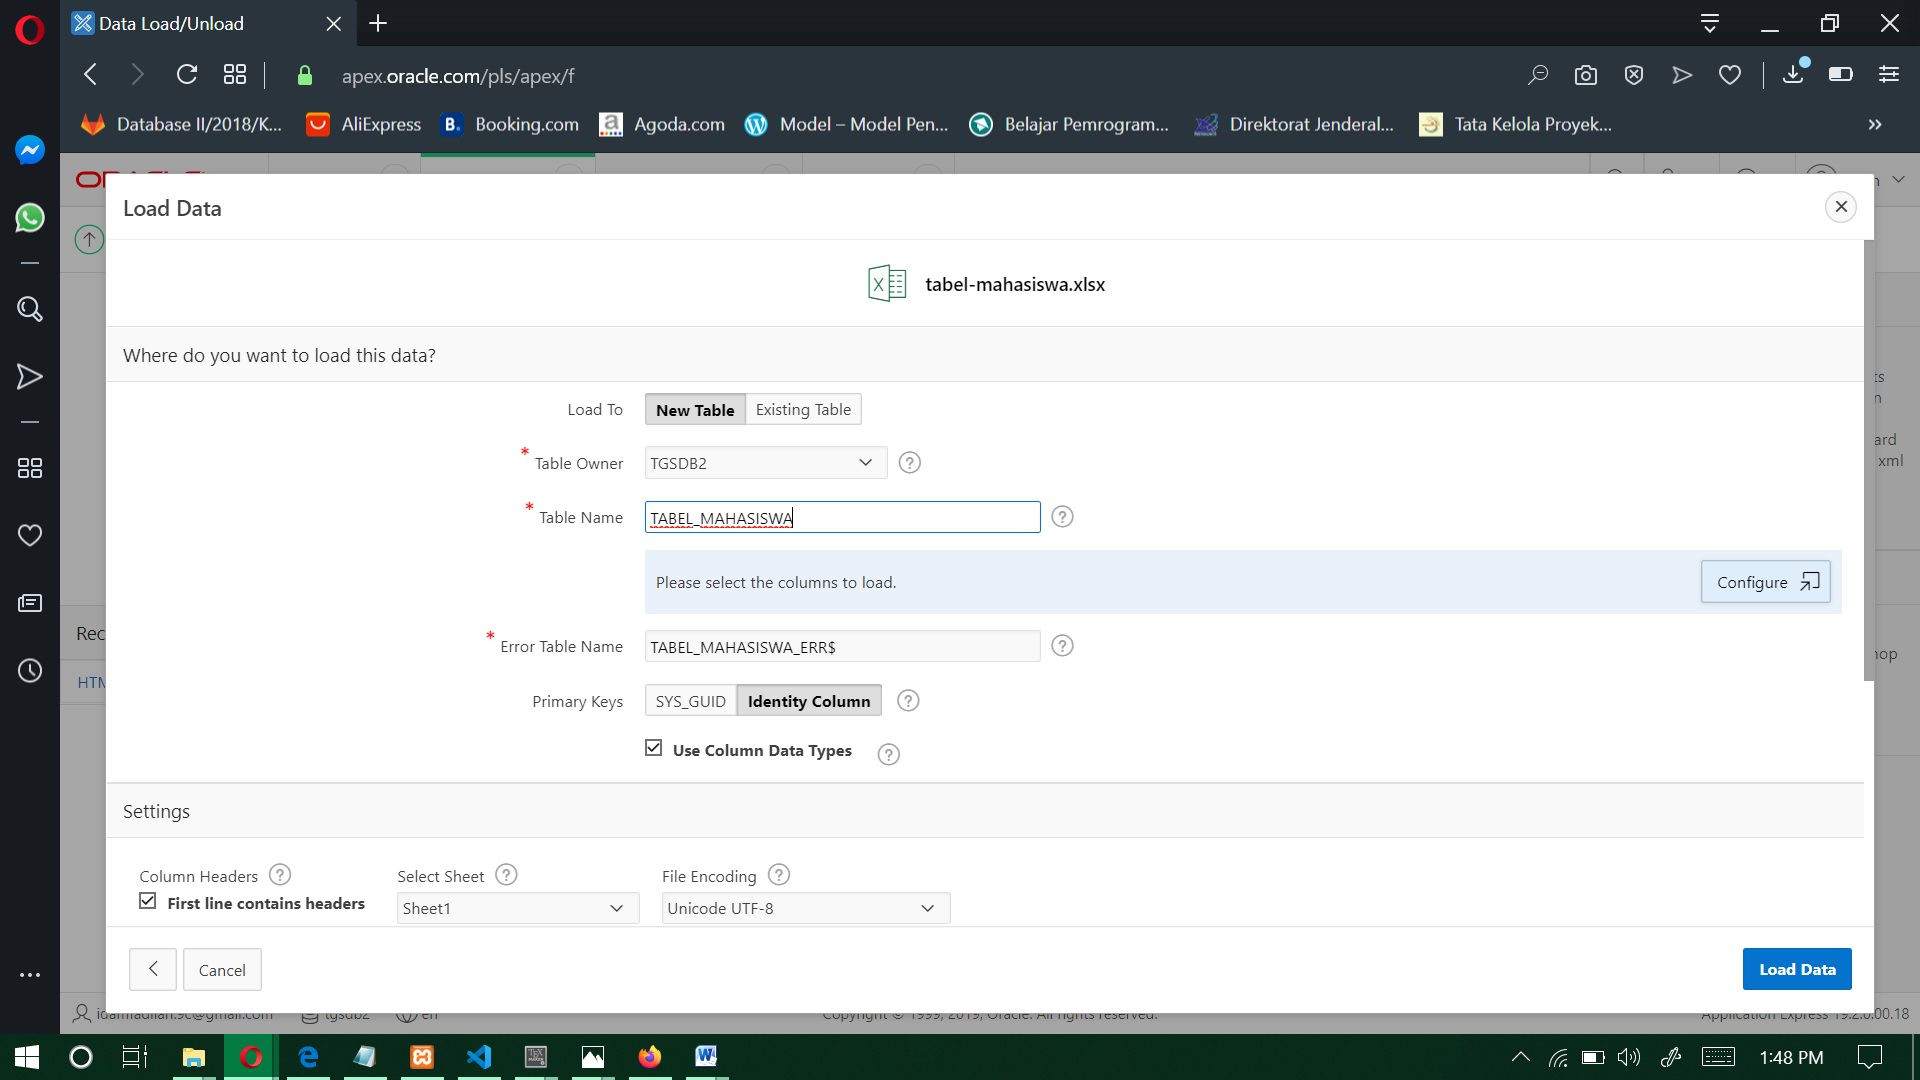
\includegraphics[width=10cm]{figures/load data csv/Screenshot (211).png} 
    \caption{\textit{form pembuatan tabel}}
    \label{foto18}
 	\end{figure}
	\item muncul tampilan seperti dibawah, pada menu ini kalian bisa memilih kolom mana yang akan dipakai, hilangkan cetang pada kolom yang tidak akan dipakai, karena disini semua kolom akan dipakai maka langsung saja klik "Save Changes".
	\begin{figure}[H]
    \centering
	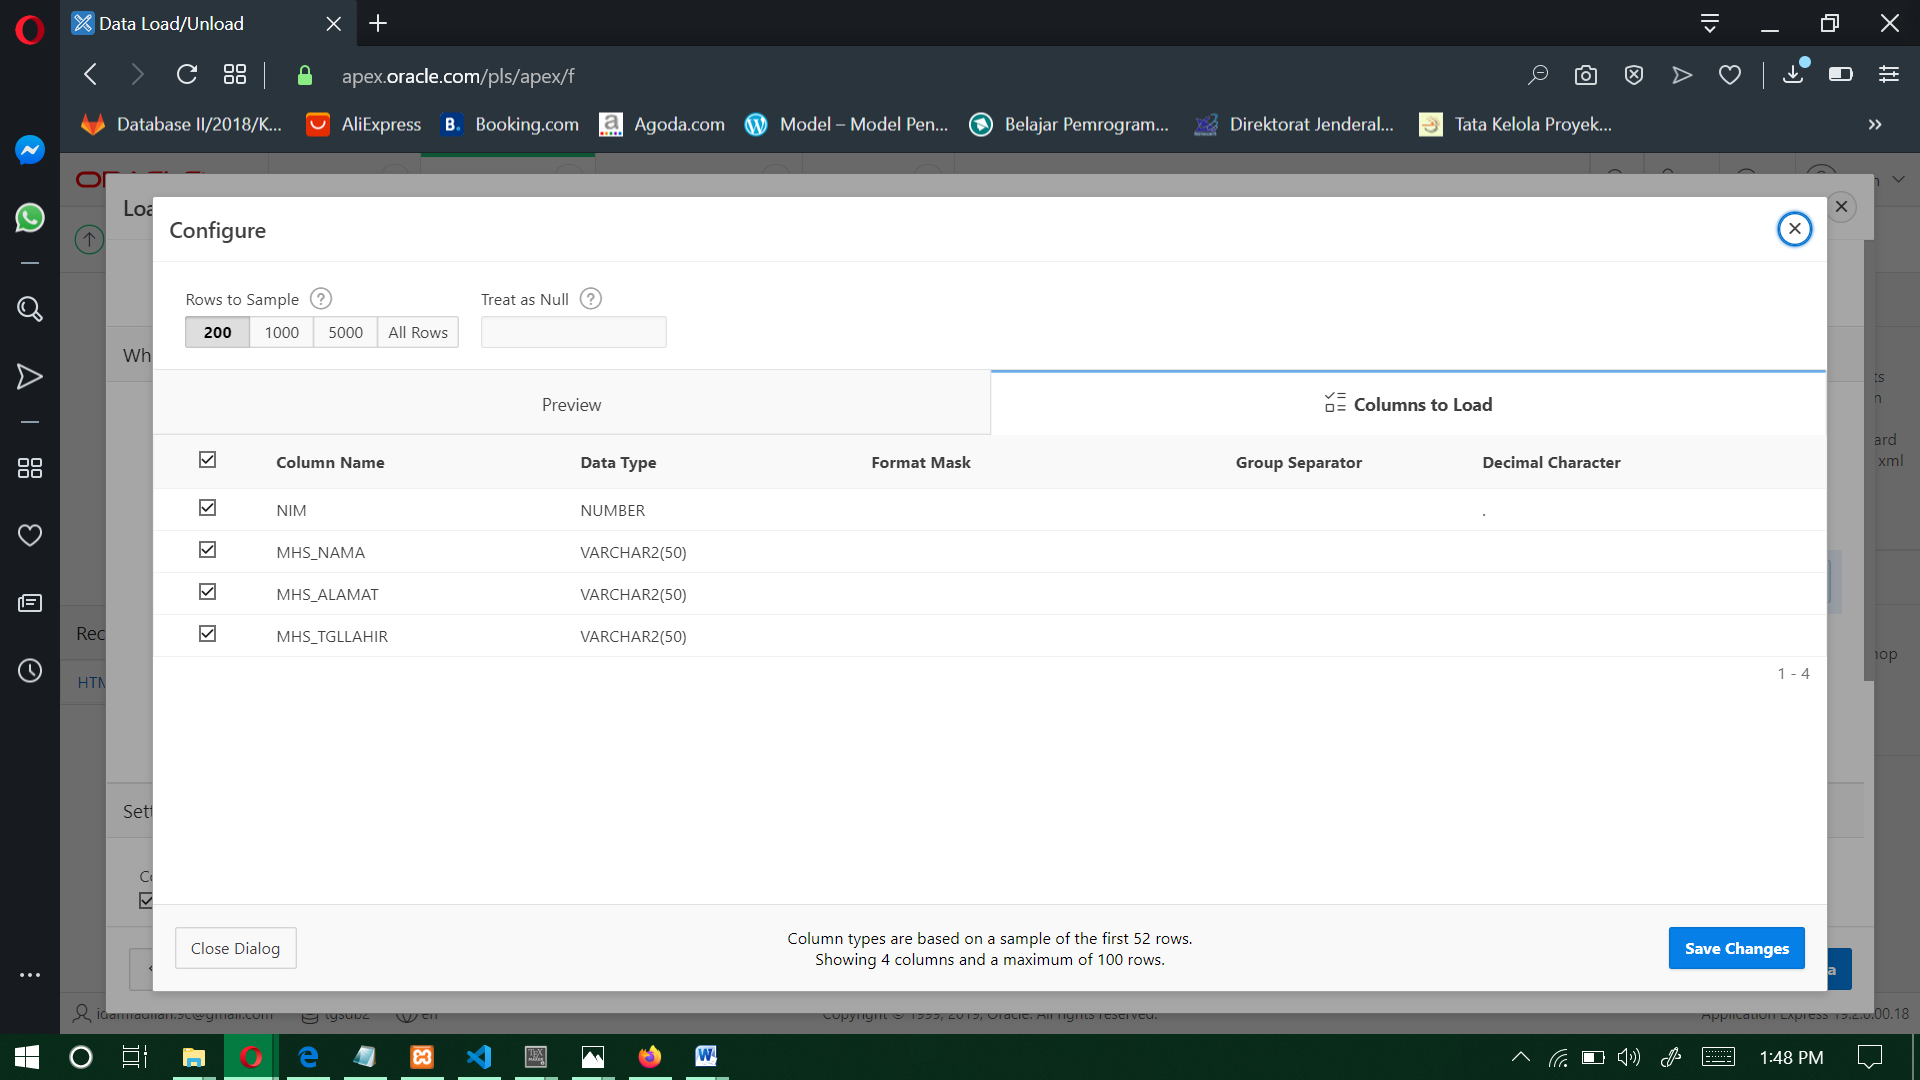
\includegraphics[width=10cm]{figures/load data csv/Screenshot (213).png} 
    \caption{\textit{konfigurasi tabel}}
    \label{foto19}
 	\end{figure}
	\item lalu jika sudah maka klik "Load Data"
	\begin{figure}[H]
    \centering
	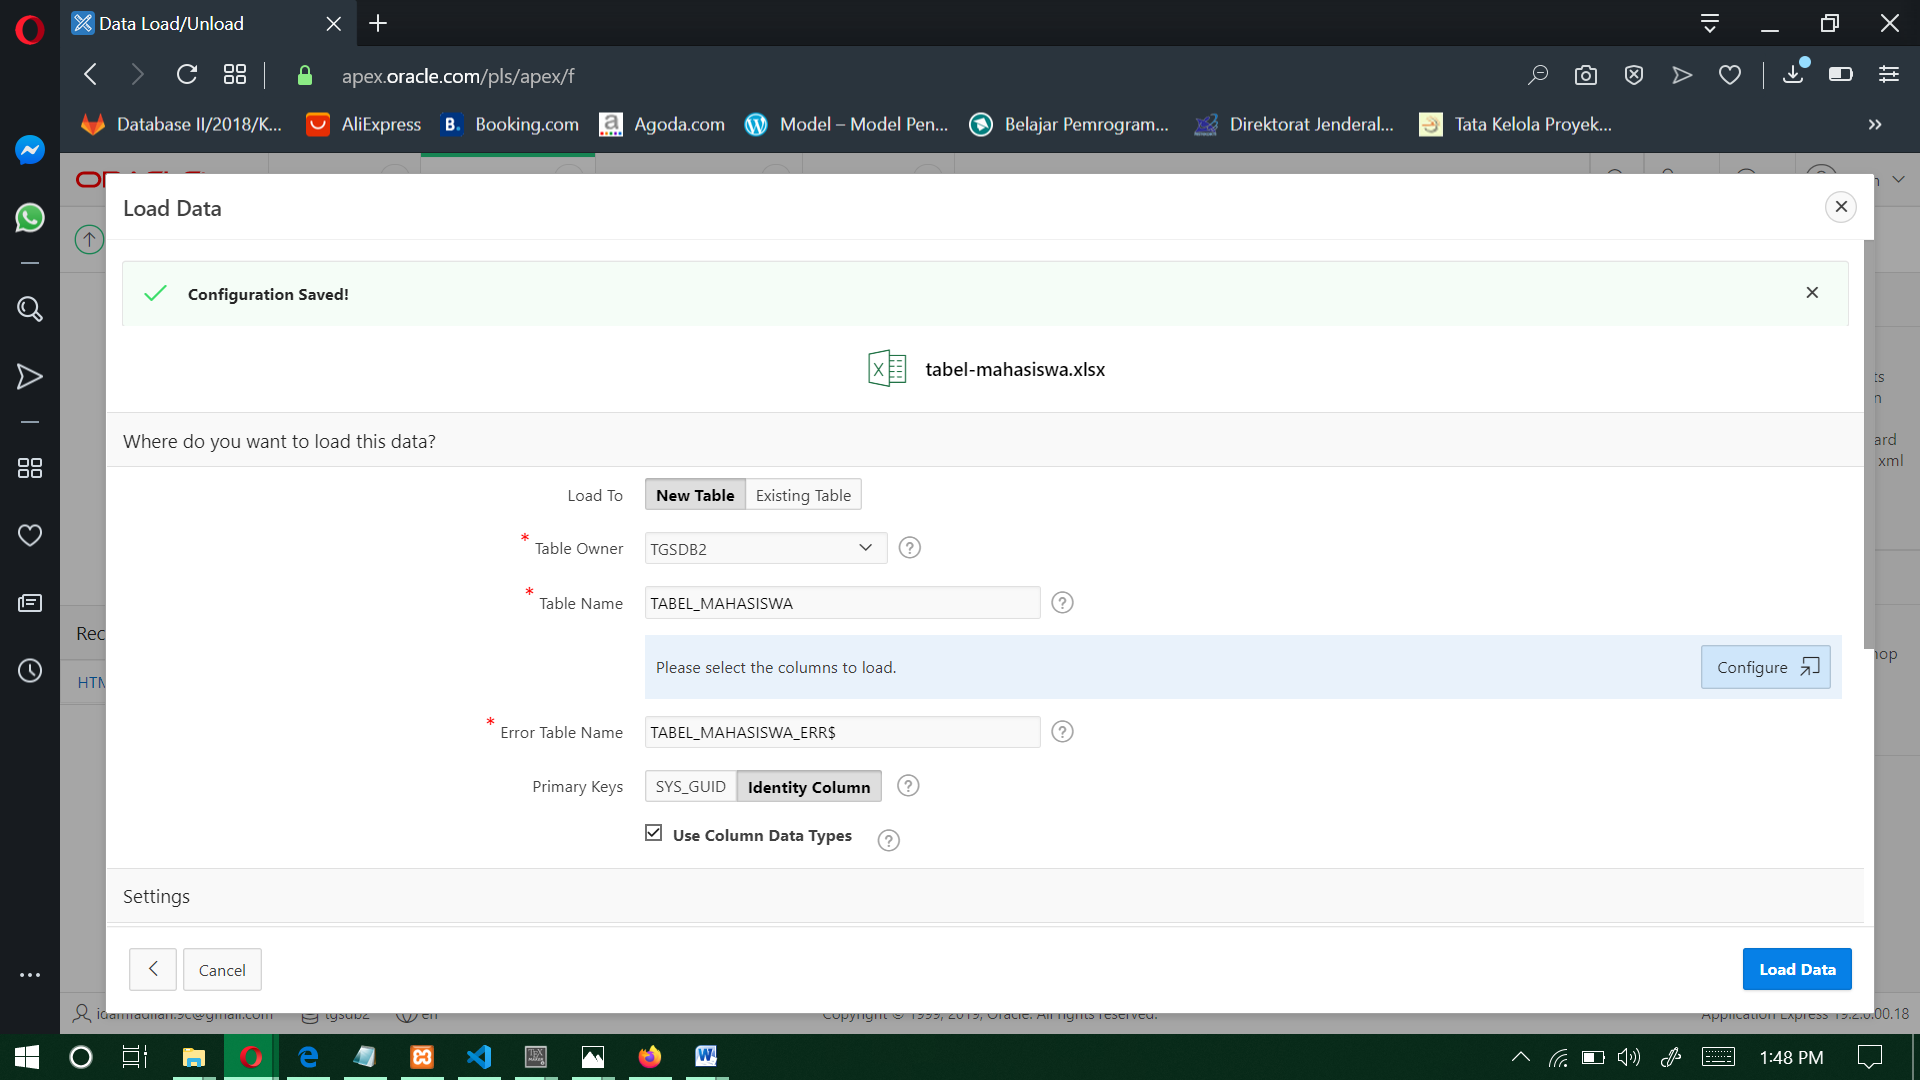
\includegraphics[width=10cm]{figures/load data csv/Screenshot (214).png} 
    \caption{\textit{form pembuatan tabel}}
    \label{foto20}
 	\end{figure}
	\item tabel sudah berhasil dibuat, lalu klik close (x).
	\begin{figure}[H]
    \centering
	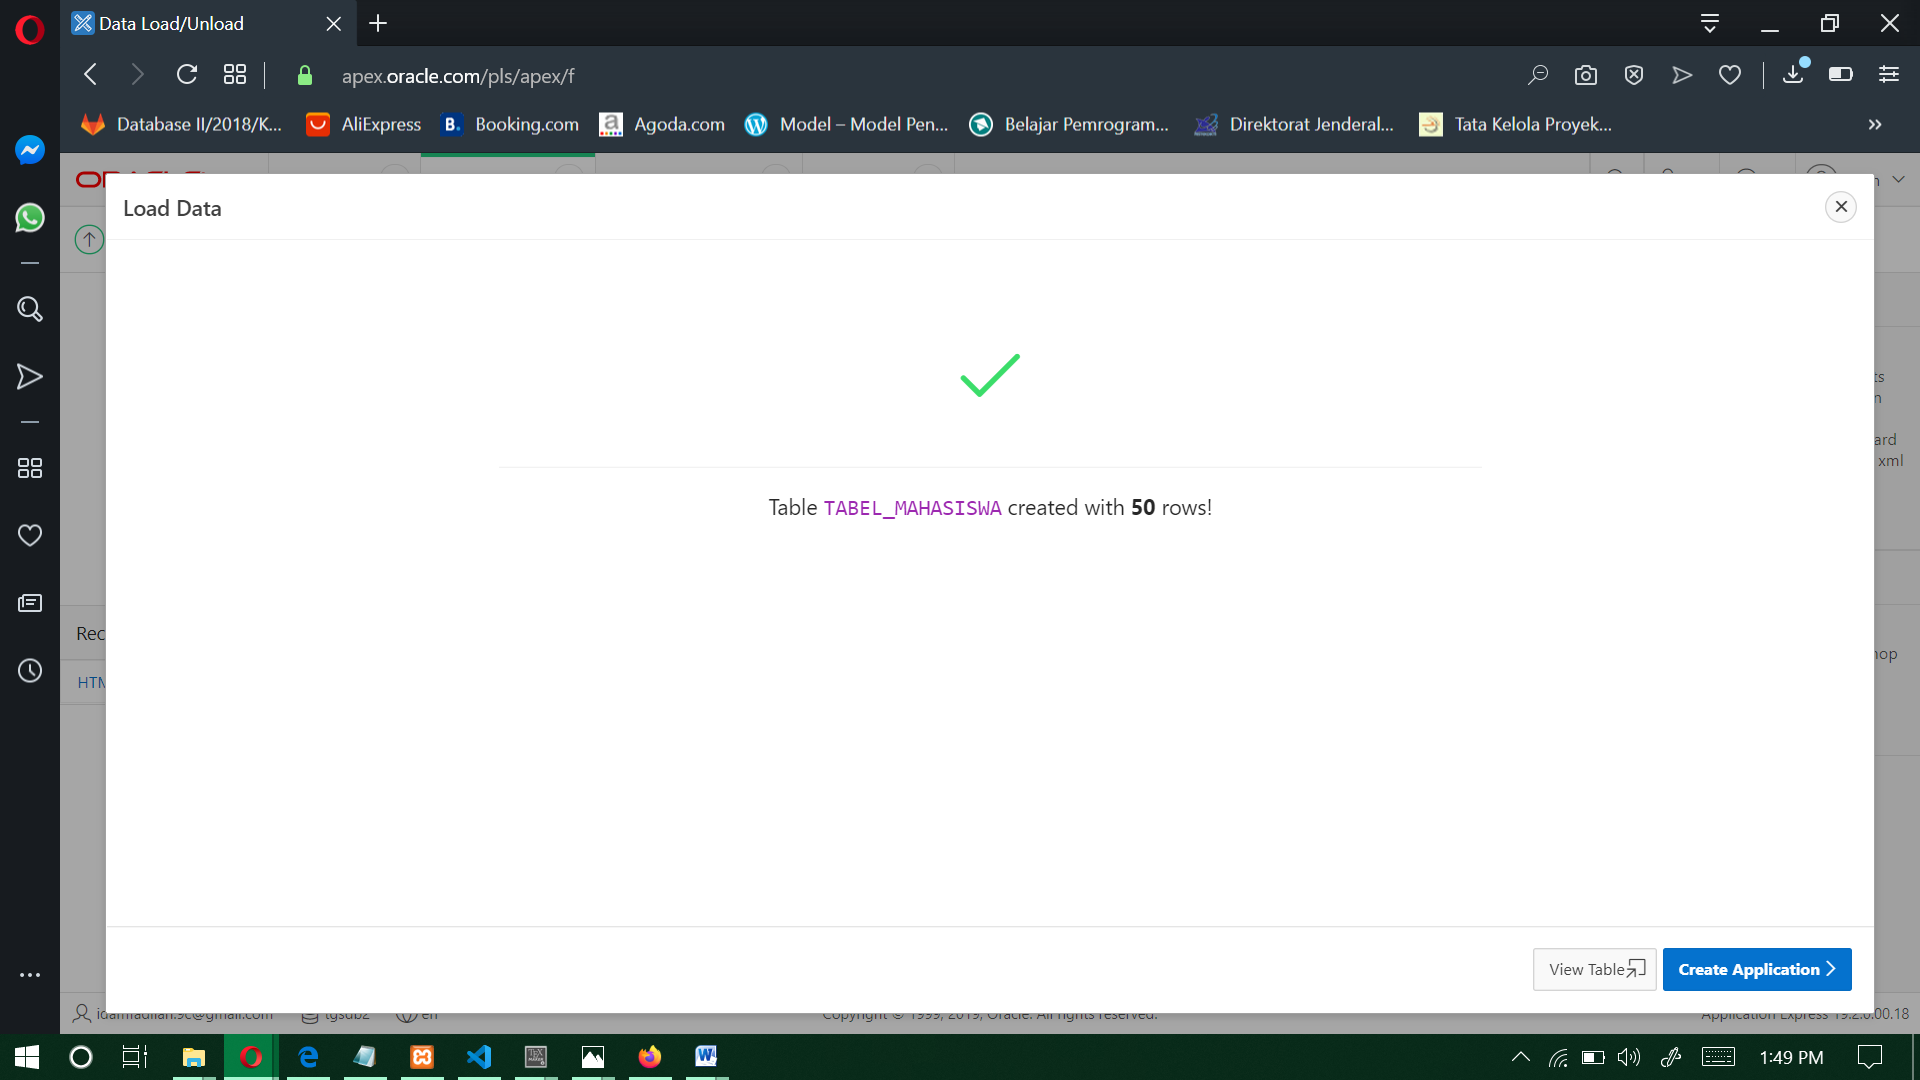
\includegraphics[width=10cm]{figures/load data csv/Screenshot (215).png} 
    \caption{\textit{tabel berhasil dibuat}}
    \label{foto21}
 	\end{figure}
	\item import semua data excel yang sudah disiapkan dengan cara seperti tadi.
	
	
\end{enumerate}
\section{relasi antar tabel}
\paragraph{}
kita telah membuat 5 tabel dari data excel yang telah disiapkan sebelumnya, selanjutnya yaitu membuat relasi antar tabel, pada tabel nilai terdapat kolom "nim" juga "kode\_matakuliah", dan pada tabel jadwal terdapat kolom "kode\_dosen" juga "kode\_matakuliah", nantinya kolom-kolom tersebut akan dibuat menjadi \textit{foreign key} yang akan dihubungkan dengan \textit{primary key} pada setiap tabel. 
\subsection{menghapus primary key default}
\paragraph{}
sebelum membuat relasi kita harus menghapus primary key default pada setiap tabel, pada saat kita membuat tabel dengan data dari excel maka APEX akan otomatis membuatkan sebuah primary key yaitu "ID" karena itu kita harus menghapus kolom ini terlebih dahulu, caranya sebagai berikut :
\begin{enumerate}
	\item klik dropdown pada "SQL Workshop" lalu pilih "SQL Commands".
	\begin{figure}[H]
    \centering
	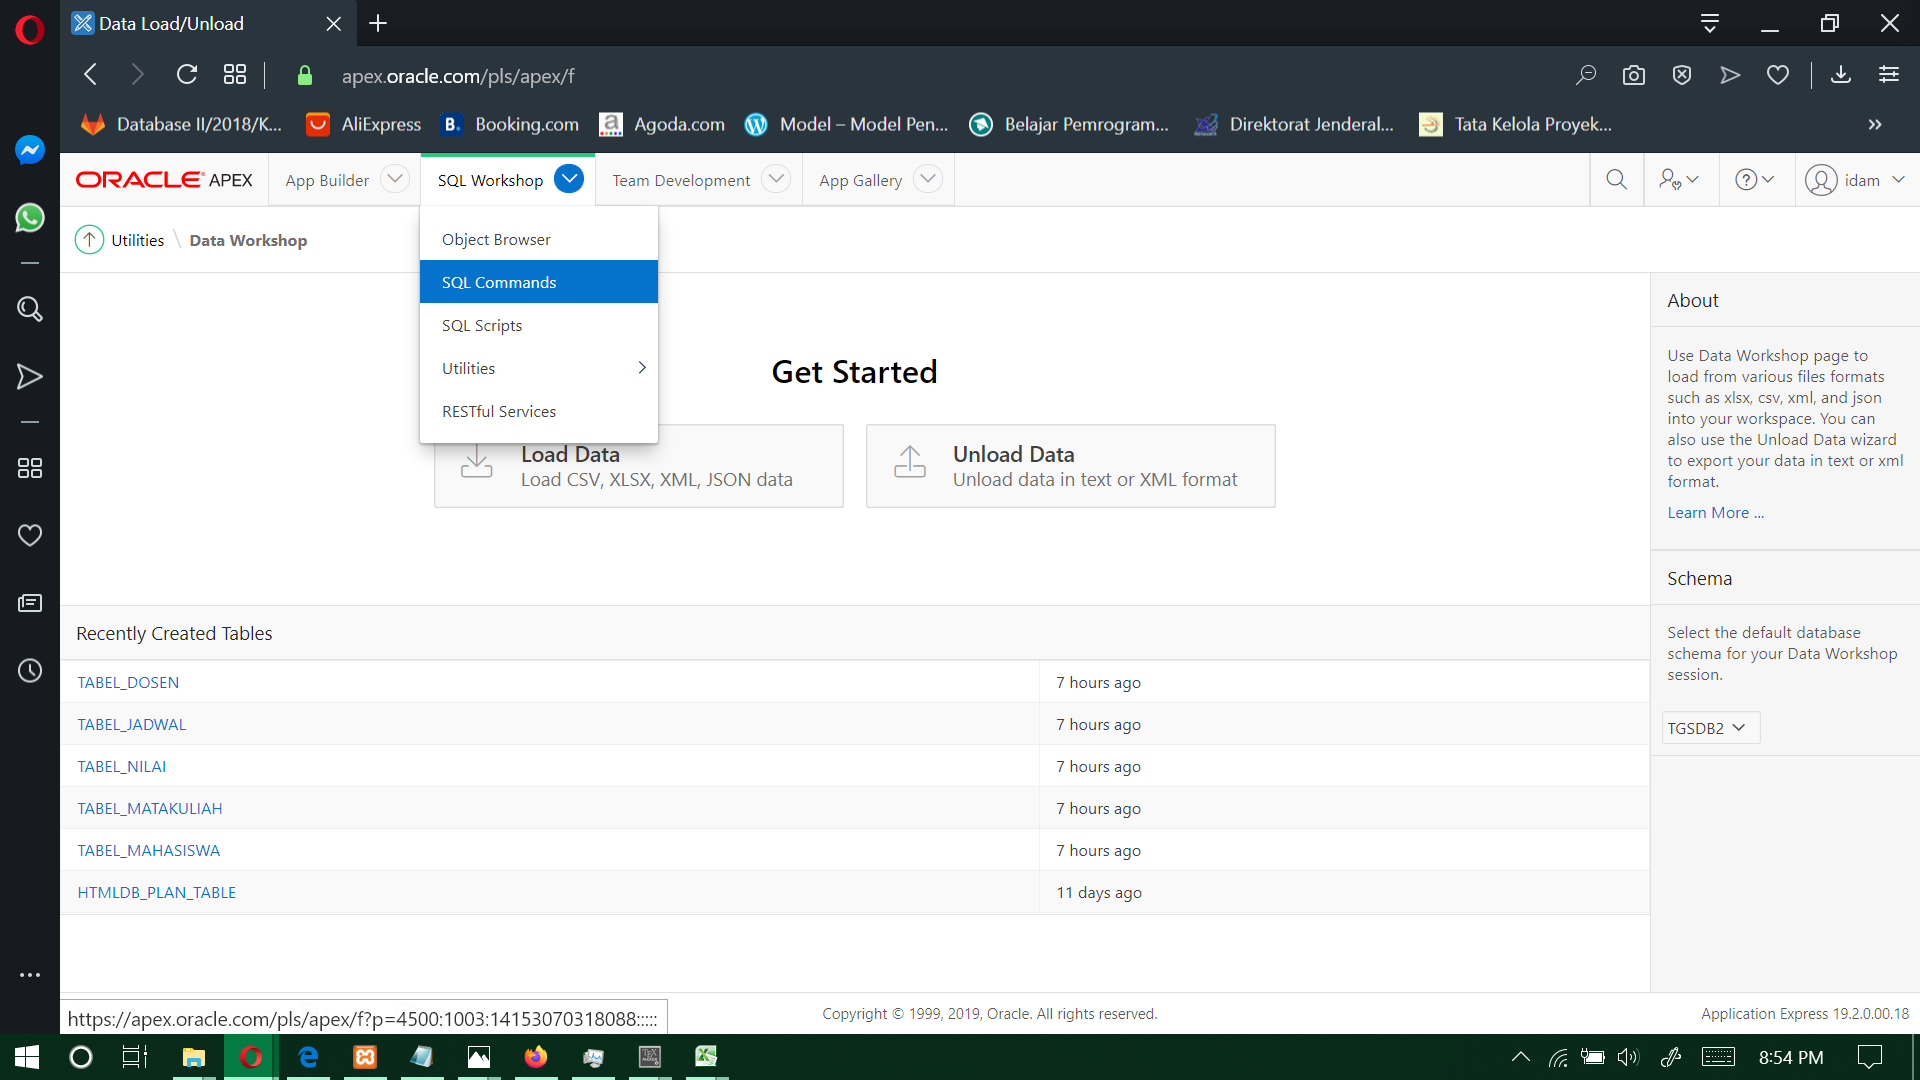
\includegraphics[width=10cm]{figures/SQL commands/Screenshot (230).png} 
    \caption{\textit{oracle apex - data workshop}}
    \label{foto21}
 	\end{figure}
	\item untuk menghapus sebuah kolom bisa menggunakan command seperti ini, lalu klik "run"
	\begin{verbatim}
	alter table drop nama_tabel column nama_kolom; 
	\end{verbatim}
	\item jadi untuk menghapus kolom "ID" dari setiap tabel yang telah dibuat tadi, ketikan command berikut
	\begin{verbatim}
	alter table drop tabel_mahasiswa column id;
	alter table drop tabel_dosen column id;
	alter table drop tabel_matakuliah column id;
	alter table drop tabel_nilai column id;
	alter table drop tabel_jadwal column id;
	\end{verbatim}
	\begin{figure}[H]
    \centering
	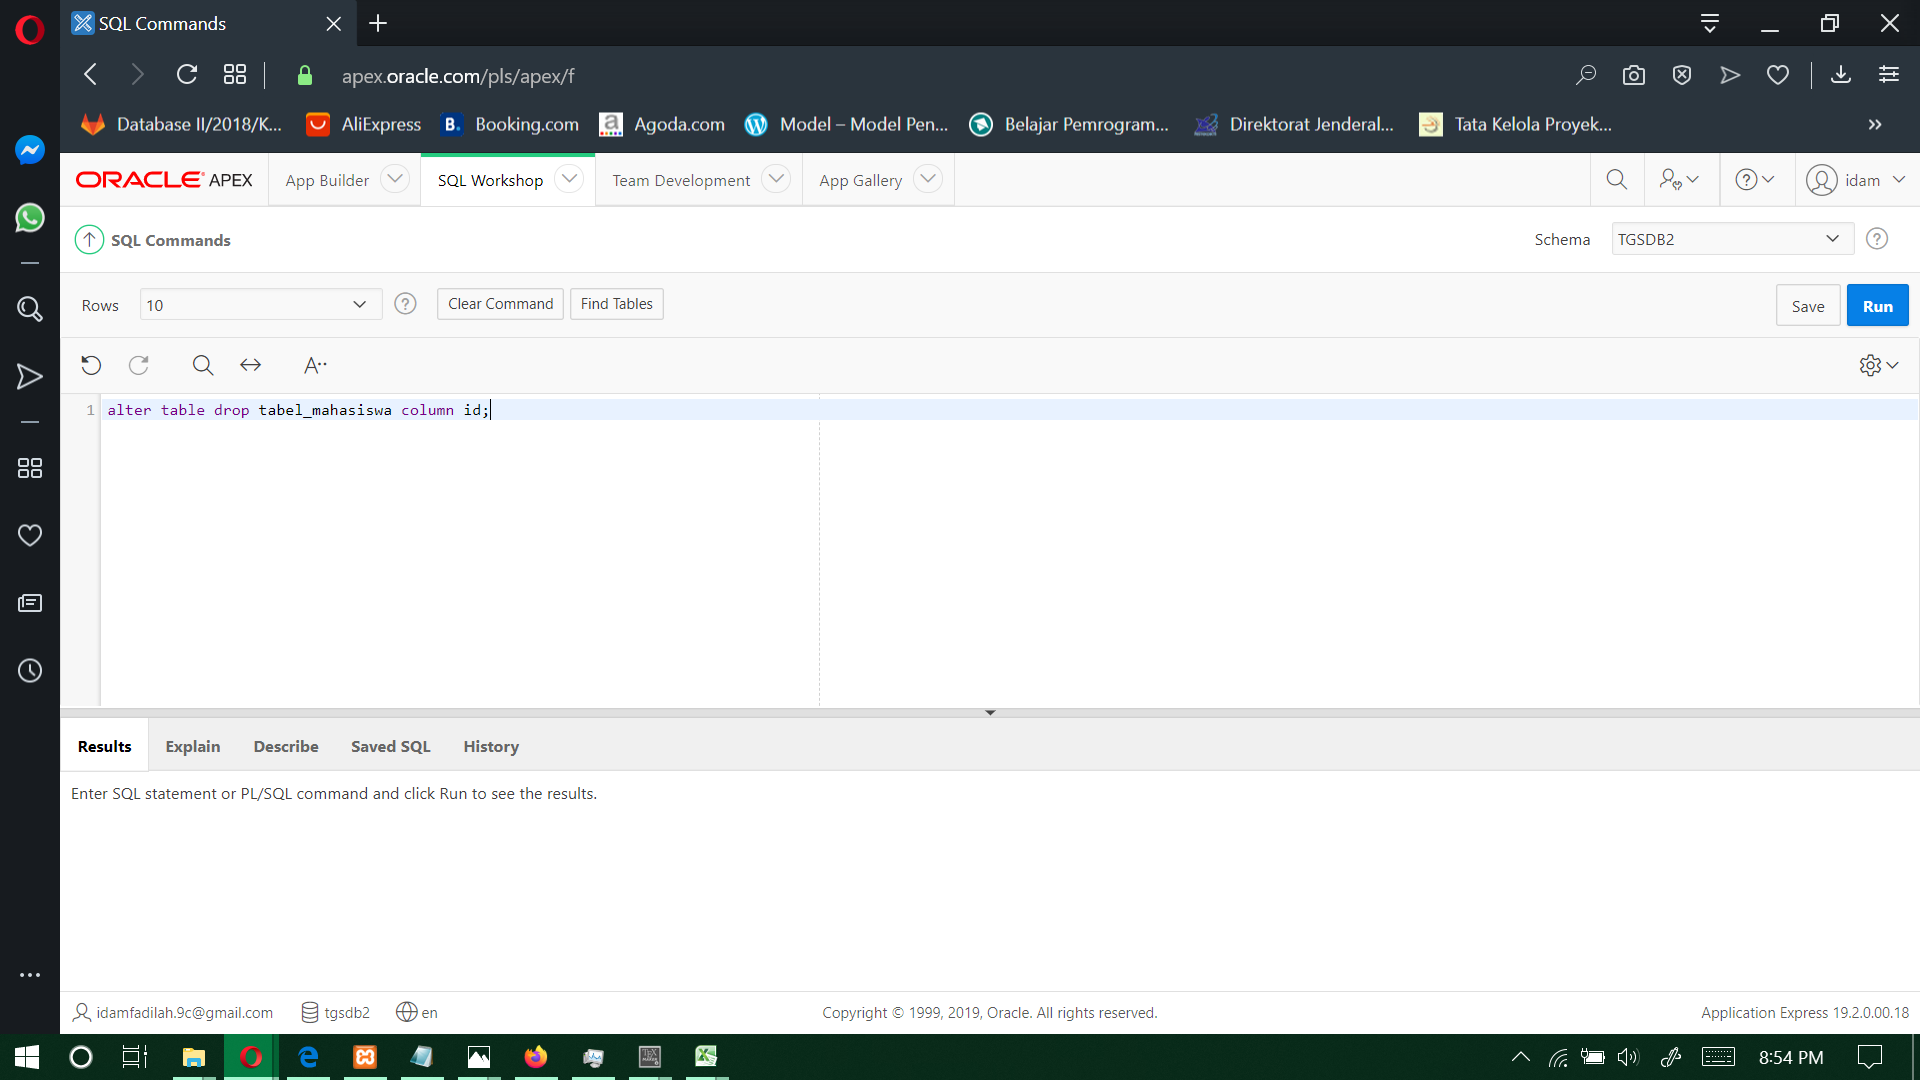
\includegraphics[width=10cm]{figures/SQL commands/Screenshot (231).png} 
    \caption{\textit{oracle apex - SQL commands}}
    \label{foto21}
 	\end{figure}	
	\end{enumerate}
\subsection{menambahkan primary key}
\paragraph{}
jika semua \textit{primary key default} sudah dihapus, maka selanjutnya membuat \textit{primary key}, perintah untuk menambahkan \textit{primary key} pada tabel :
    \begin{verbatim}
    alter table nama_tabel
    add primary key (nama_kolom);
    \end{verbatim}
tambahkan \textit{primary key} pada tabel mahasiswa, dosen, dan matakuliah. perlu diingat bahwa \textit{primary key} harus bersifat unique, pada tabel-tabel tersebut masing-masing sudah mempunyai kolom yang datanya bersifat unique,pada tabel mahasiswa terdapat "nim", pada tabel dosen terdapat "kode\_dosen" dan pada tabel matakuliah terdapat "kode\_matakuliah", kalau \textit{primary key} sudah ditentukan tinggal membuatnya,  masih dalam menu "SQL Commands", ketikan perintah berikut :
    \begin{verbatim}
     alter table tabel_mahasiswa
     add primary key (nim);

     alter table tabel_dosen
     add primary key (kode_dosen);

     alter table tabel_matakuliah
     add primary key (kode_matakuliah);
	\end{verbatim}
	\begin{figure}[H]
    \centering
	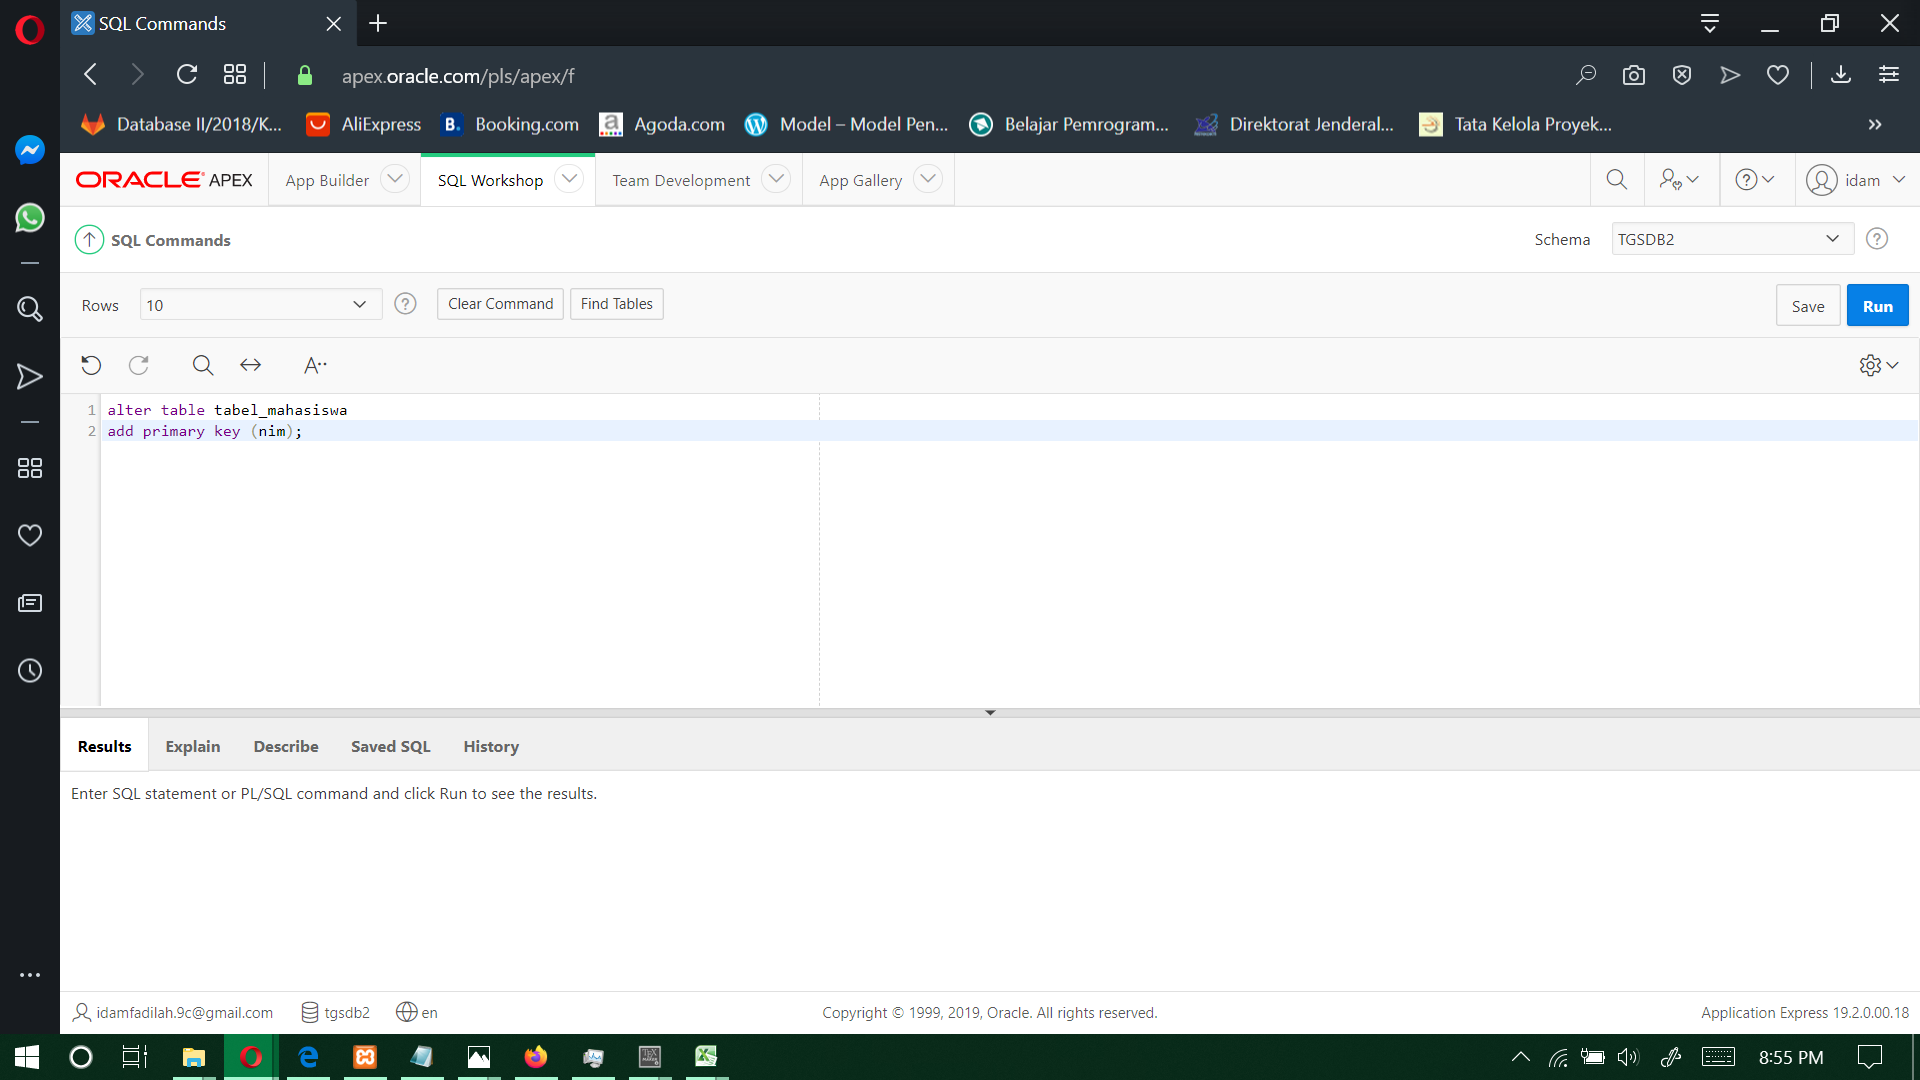
\includegraphics[width=10cm]{figures/SQL commands/Screenshot (232).png} 
    \caption{\textit{oracle apex - SQL commands}}
    \label{foto21}
 	\end{figure}	
\subsection{menambahkan foreign key}
\paragraph{}
jika sudah beres menambahkan \textit{primary key}, maka selanjutnya menambahkan \textit{foreign key}, perintah untuk menambahkan \textit{foreign key} pada tabel :
	\begin{verbatim}
	alter table nama_tabel
	add foreign key (nama_kolom)
	references nama_tabel_sumber (nama_kolom);
    \end{verbatim}
tambahkan \textit{foreign key} pada tabel nilai pada kolom "nim" juga "kode\_matakuliah" dan pada tabel jadwal pada kolom "kode\_dosen" juga "kode\_matakuliah", masih dalam menu "SQL Commands", ketikan perintah berikut :
	\begin{verbatim}
	alter table tabel_jadwal
	add foreign key (kode_dosen)
	references tabel_dosen (kode_dosen);

	alter table tabel_jadwal
	add foreign key (kode_matakuliah)
	references tabel_matakuliah (kode_matakuliah);

	add foreign key
	alter table tabel_nilai
	add foreign key (nim)
	references tabel_mahasiswa (nim);

	alter table tabel_nilai
	add foreign key (kode_matakuliah)
	references tabel_matakuliah (kode_matakuliah);
    \end{verbatim}
    \begin{figure}[H]
    \centering
	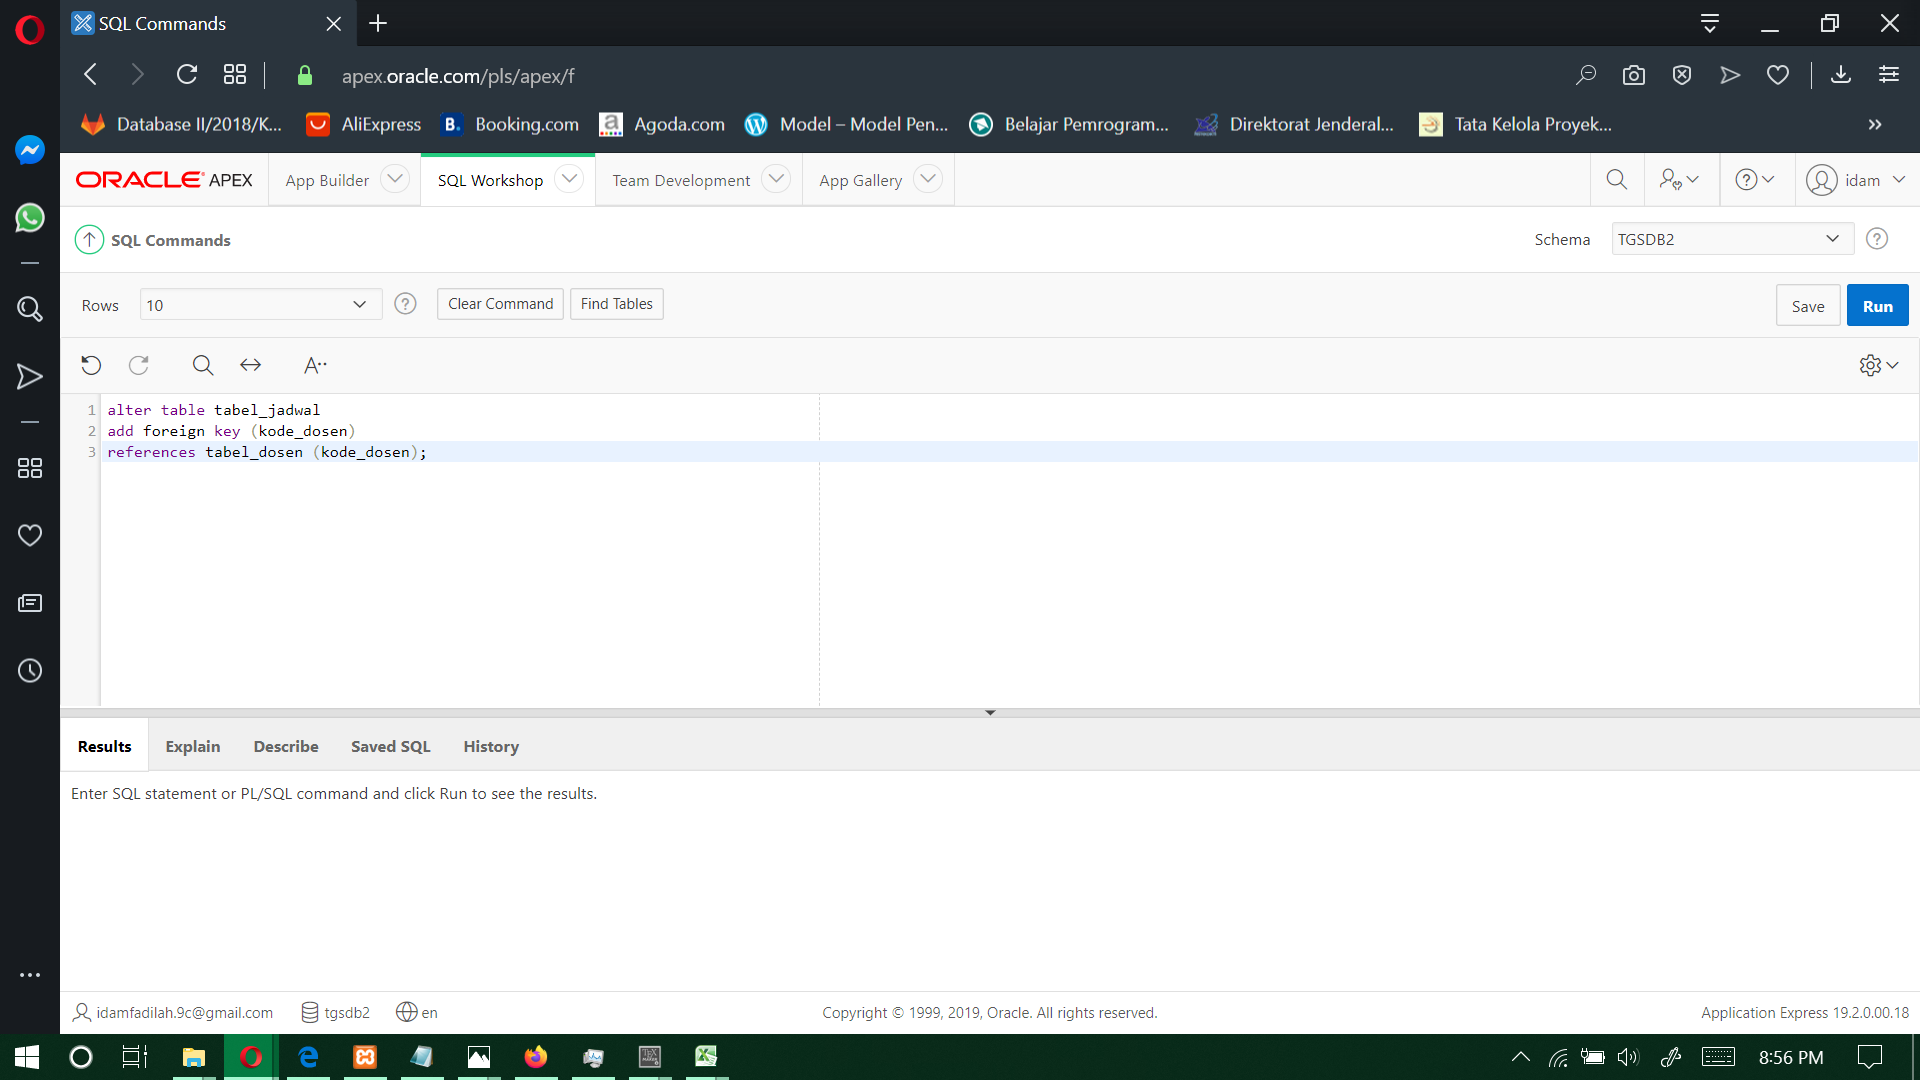
\includegraphics[width=10cm]{figures/SQL commands/Screenshot (233).png} 
    \caption{\textit{oracle apex - SQL commands}}
    \label{foto21}
 	\end{figure}	
\section{membuat aplikasi websheet}
\paragraph{}
jika semua tabel sudah siap, maka tahap selanjutnya yaitu membuat aplikasi websheet, cara membuat aplikasinya sebagai berikut :
\begin{enumerate}
	\item pertama klik dropdown "App Builder" kemudian klik "Create"
	\begin{figure}[H]
    \centering
	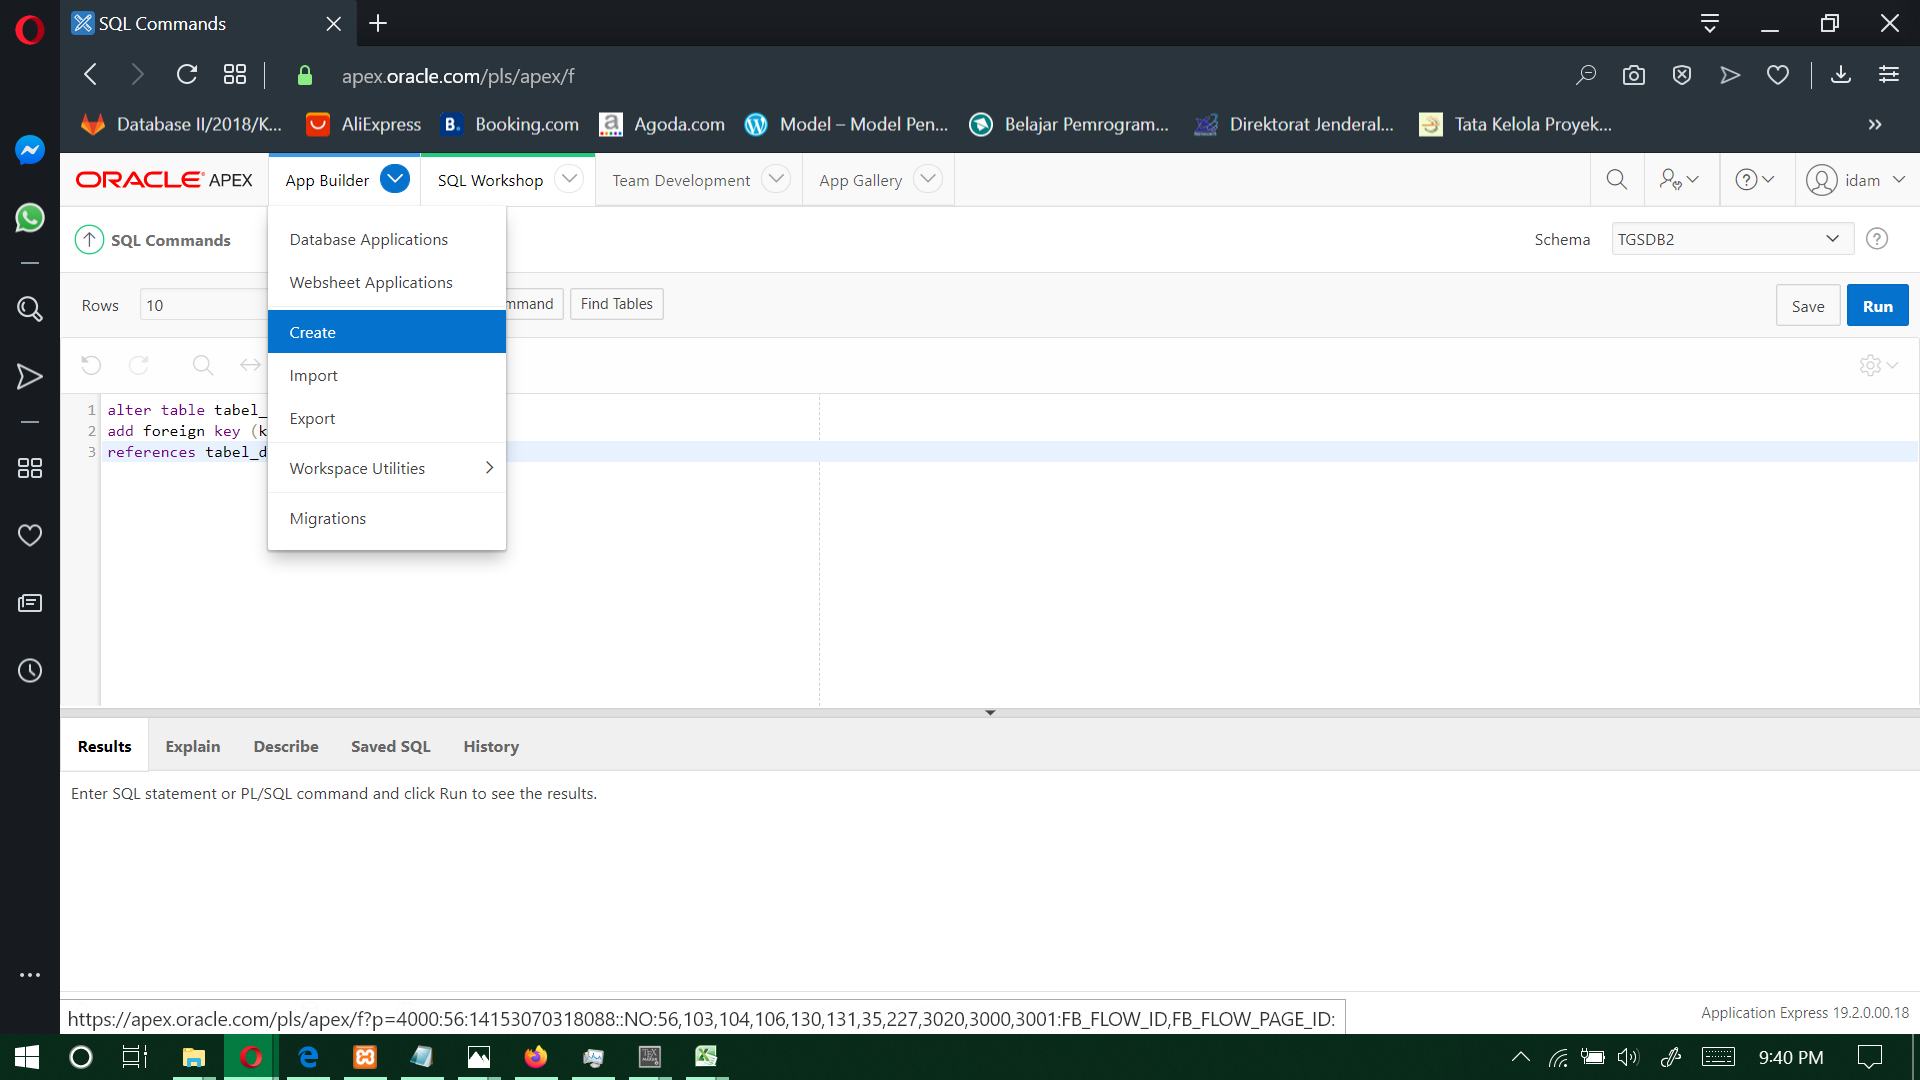
\includegraphics[width=10cm]{figures/create app/Screenshot (234).png} 
    \caption{\textit{oracle apex - SQL commands}}
    \label{foto21}
 	\end{figure}
	\item setelah itu klik "New Application"
	\begin{figure}[H]
    \centering
	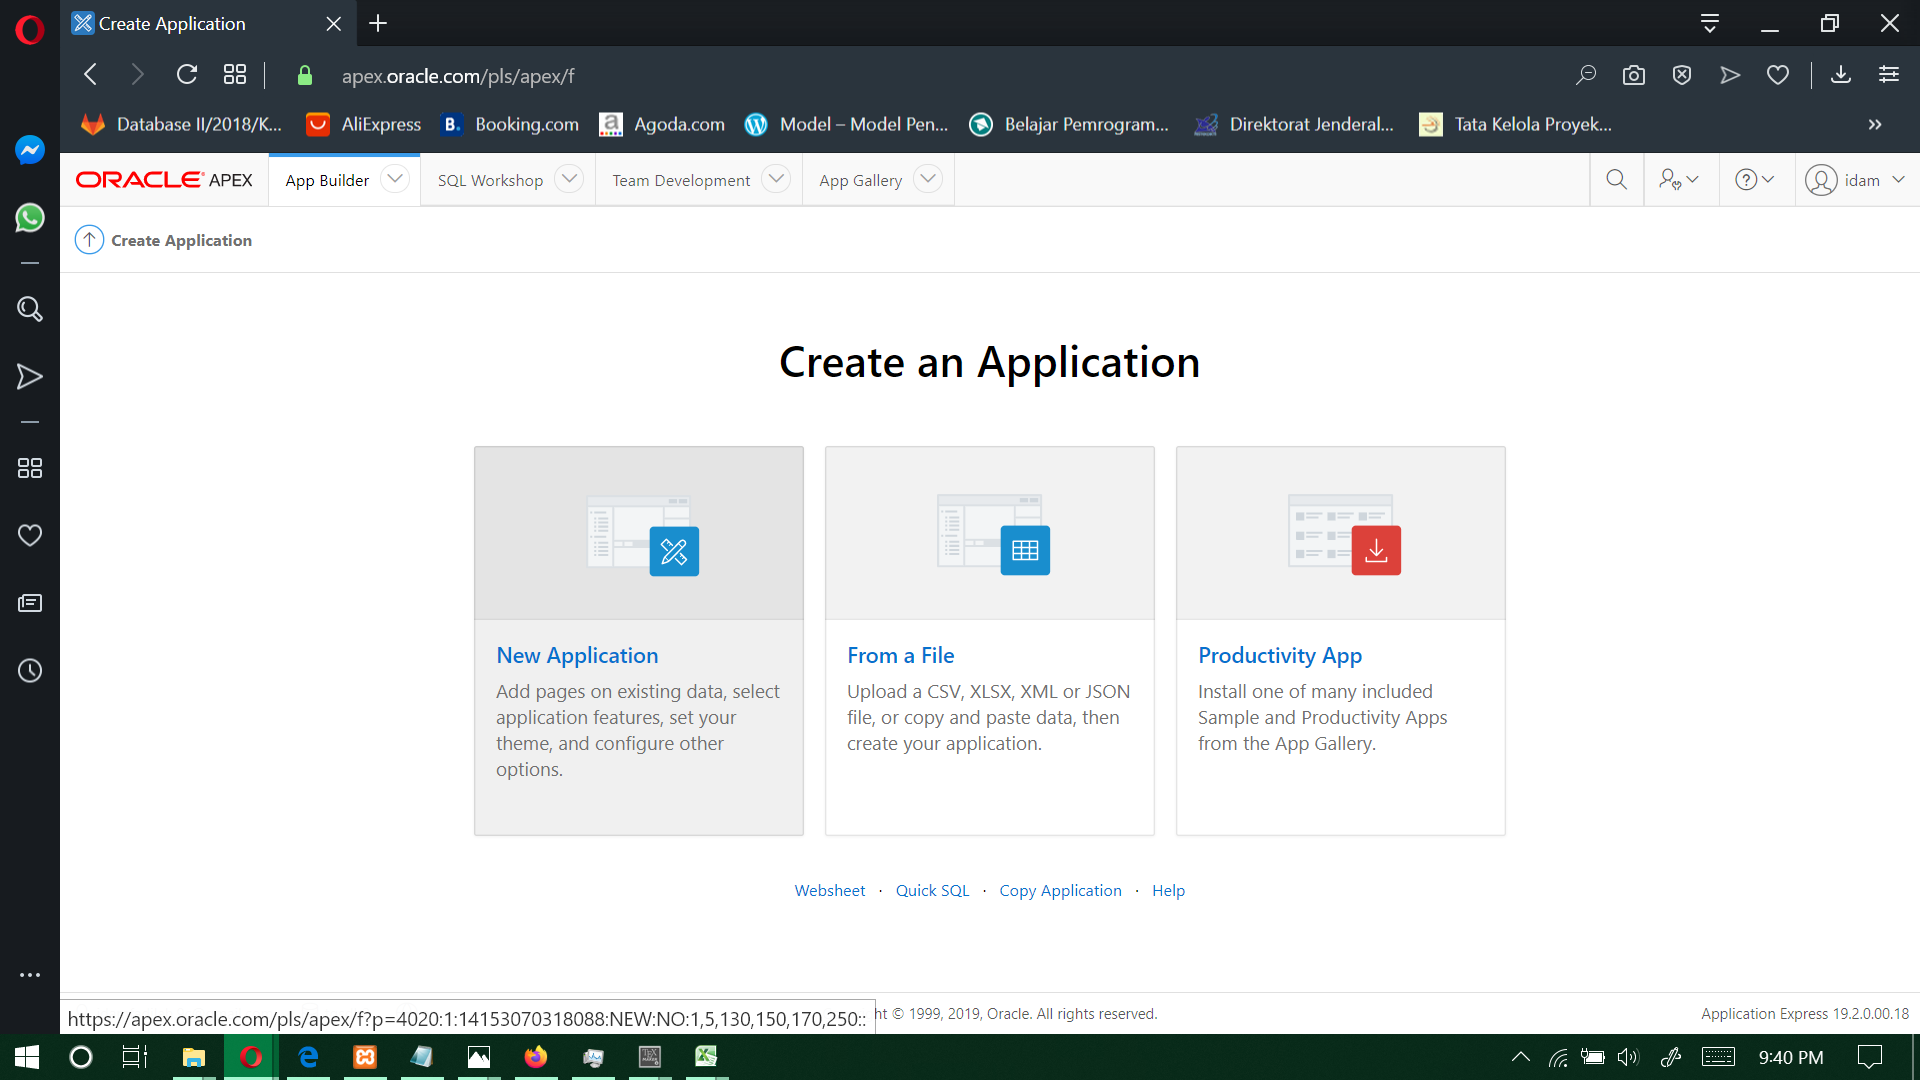
\includegraphics[width=10cm]{figures/create app/Screenshot (235).png} 
    \caption{\textit{oracle apex - App builder}}
    \label{foto21}
 	\end{figure}
	\item isi "Name"
	\begin{figure}[H]
    \centering
	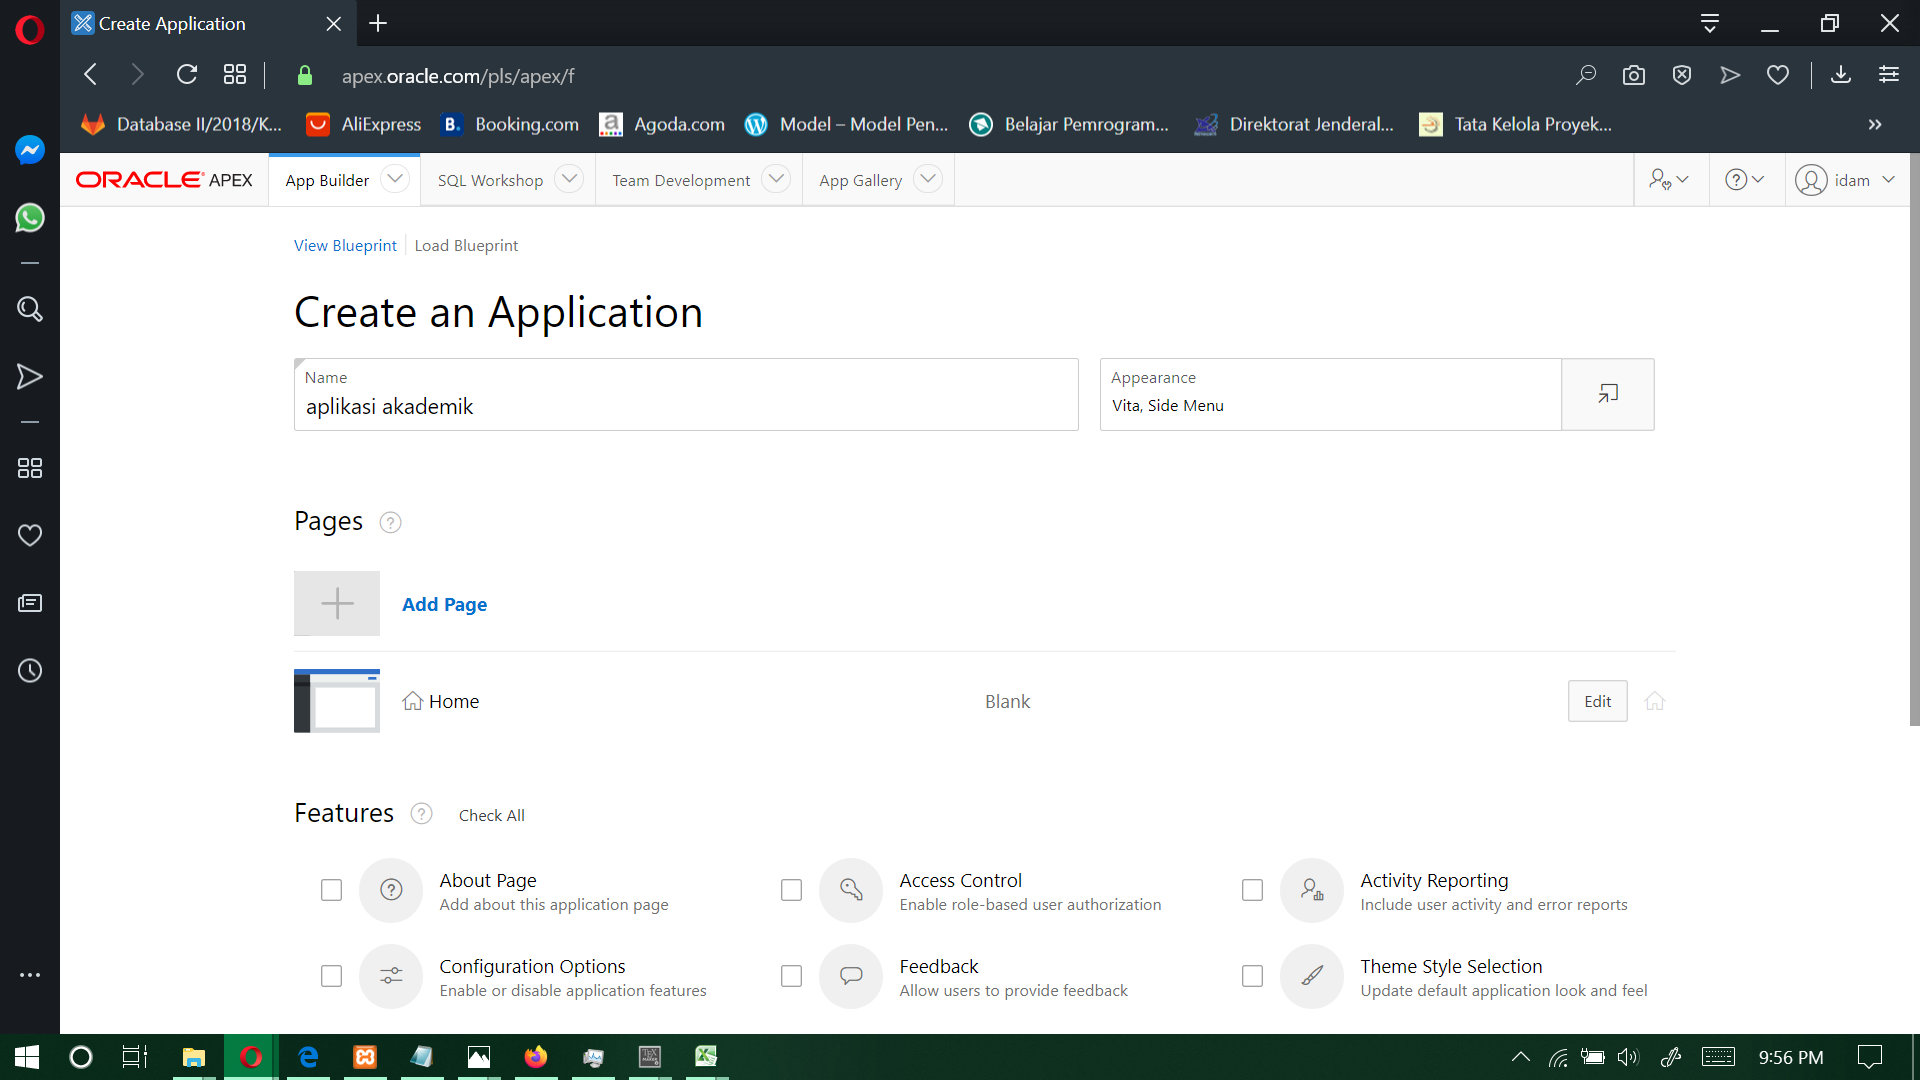
\includegraphics[width=10cm]{figures/create app/Screenshot (244).png} 
    \caption{\textit{oracle apex - App builder}}
    \label{foto21}
 	\end{figure}
	\item selanjutnya yaitu menambahkan page untuk aplikasi, pada aplikasi ini kita bisa menampilkan data berdasarkan tabel yang telah kita buat atau juga menampilkan data berdasarkan \textit{query} SQL, klik add page
\end{enumerate}
\subsection{menambahkan page dari tabel mahasiswa, dosen, dan matakuliah}
\paragraph{}
pada ketiga page ini kita akan mengambil data berdasarkan tabel saja, caranya sebagai berikut :
\begin{enumerate}
	\item klik "Add Page", pilih "interactive report"
	\begin{figure}[H]
    \centering
	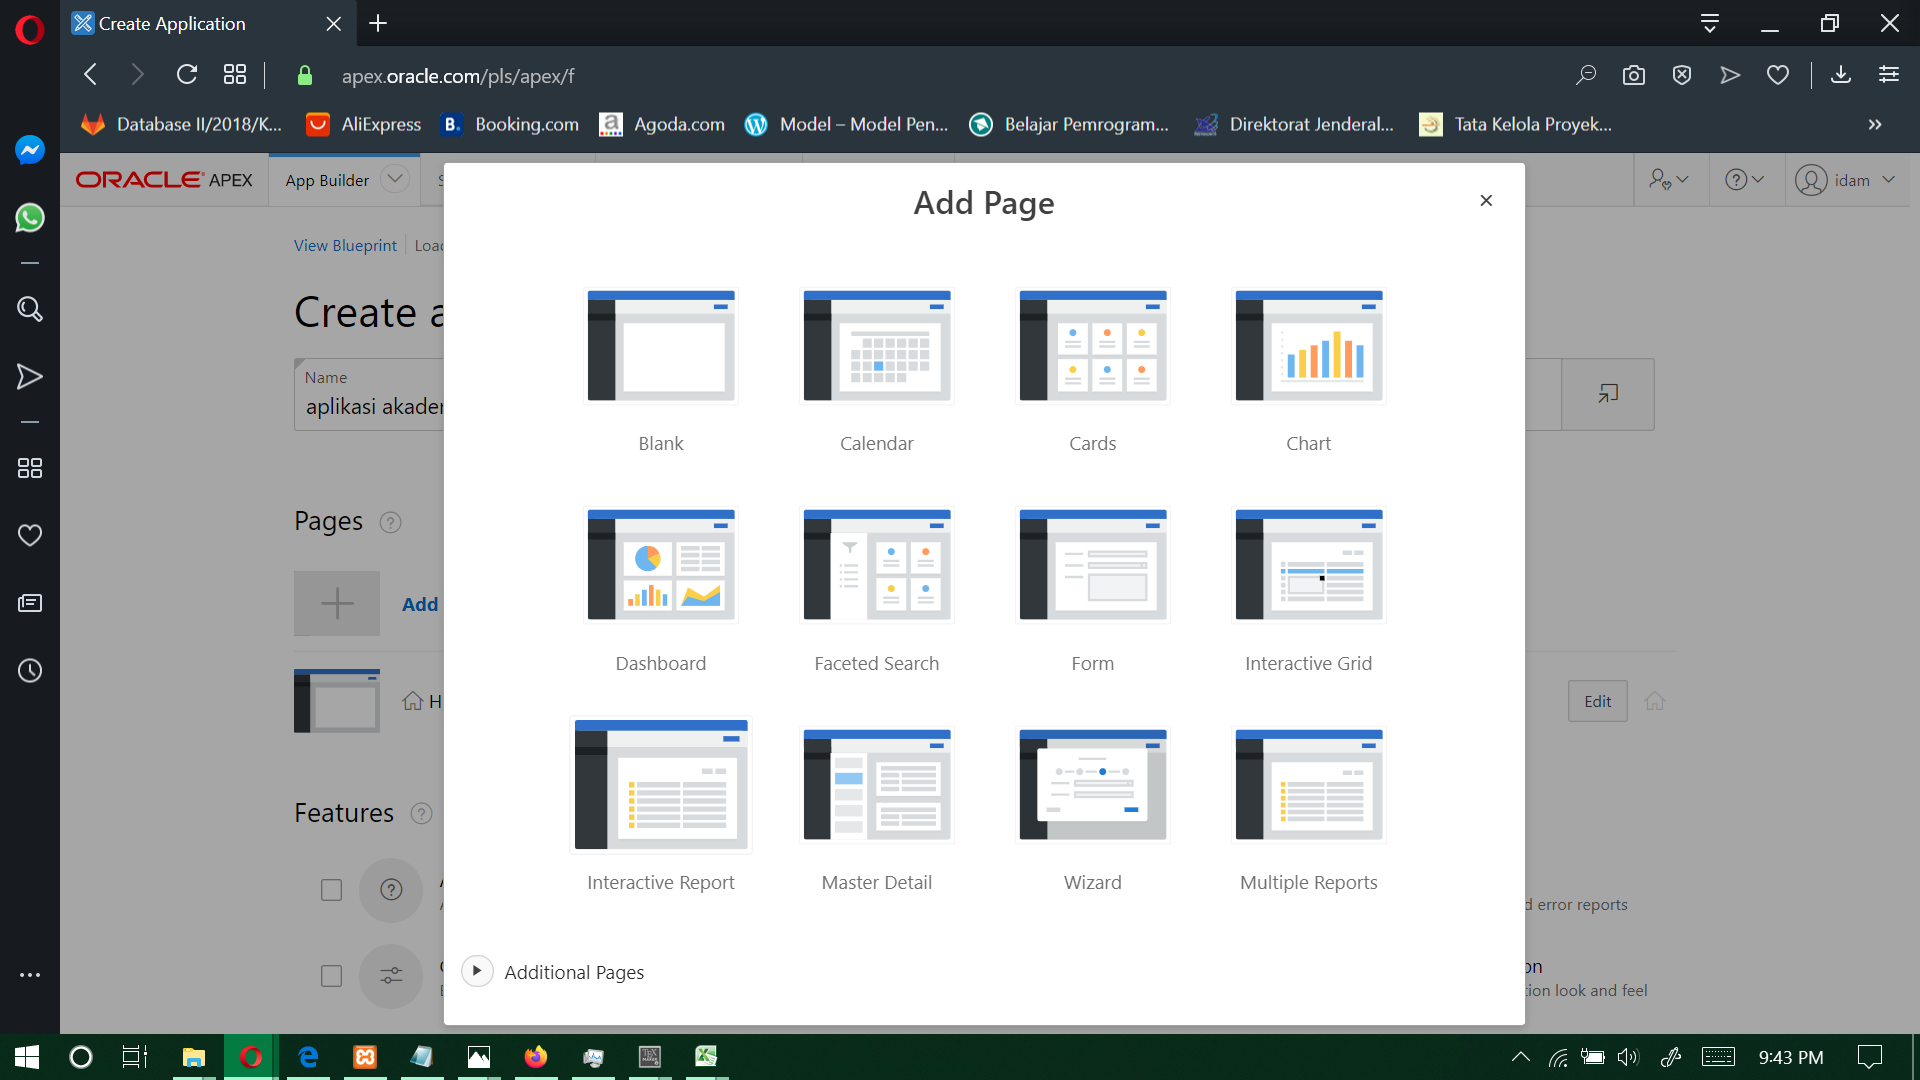
\includegraphics[width=10cm]{figures/add page/Screenshot (236).png} 
    \caption{\textit{menambahkan page pada aplikasi}}
    \label{foto21}
 	\end{figure}
	\item isi "Page Name" kemudian pilih tabel yang akan digunakan dengan cara klik tombol pada "Table or View" sebelah kanan
	\begin{figure}[H]
    \centering
    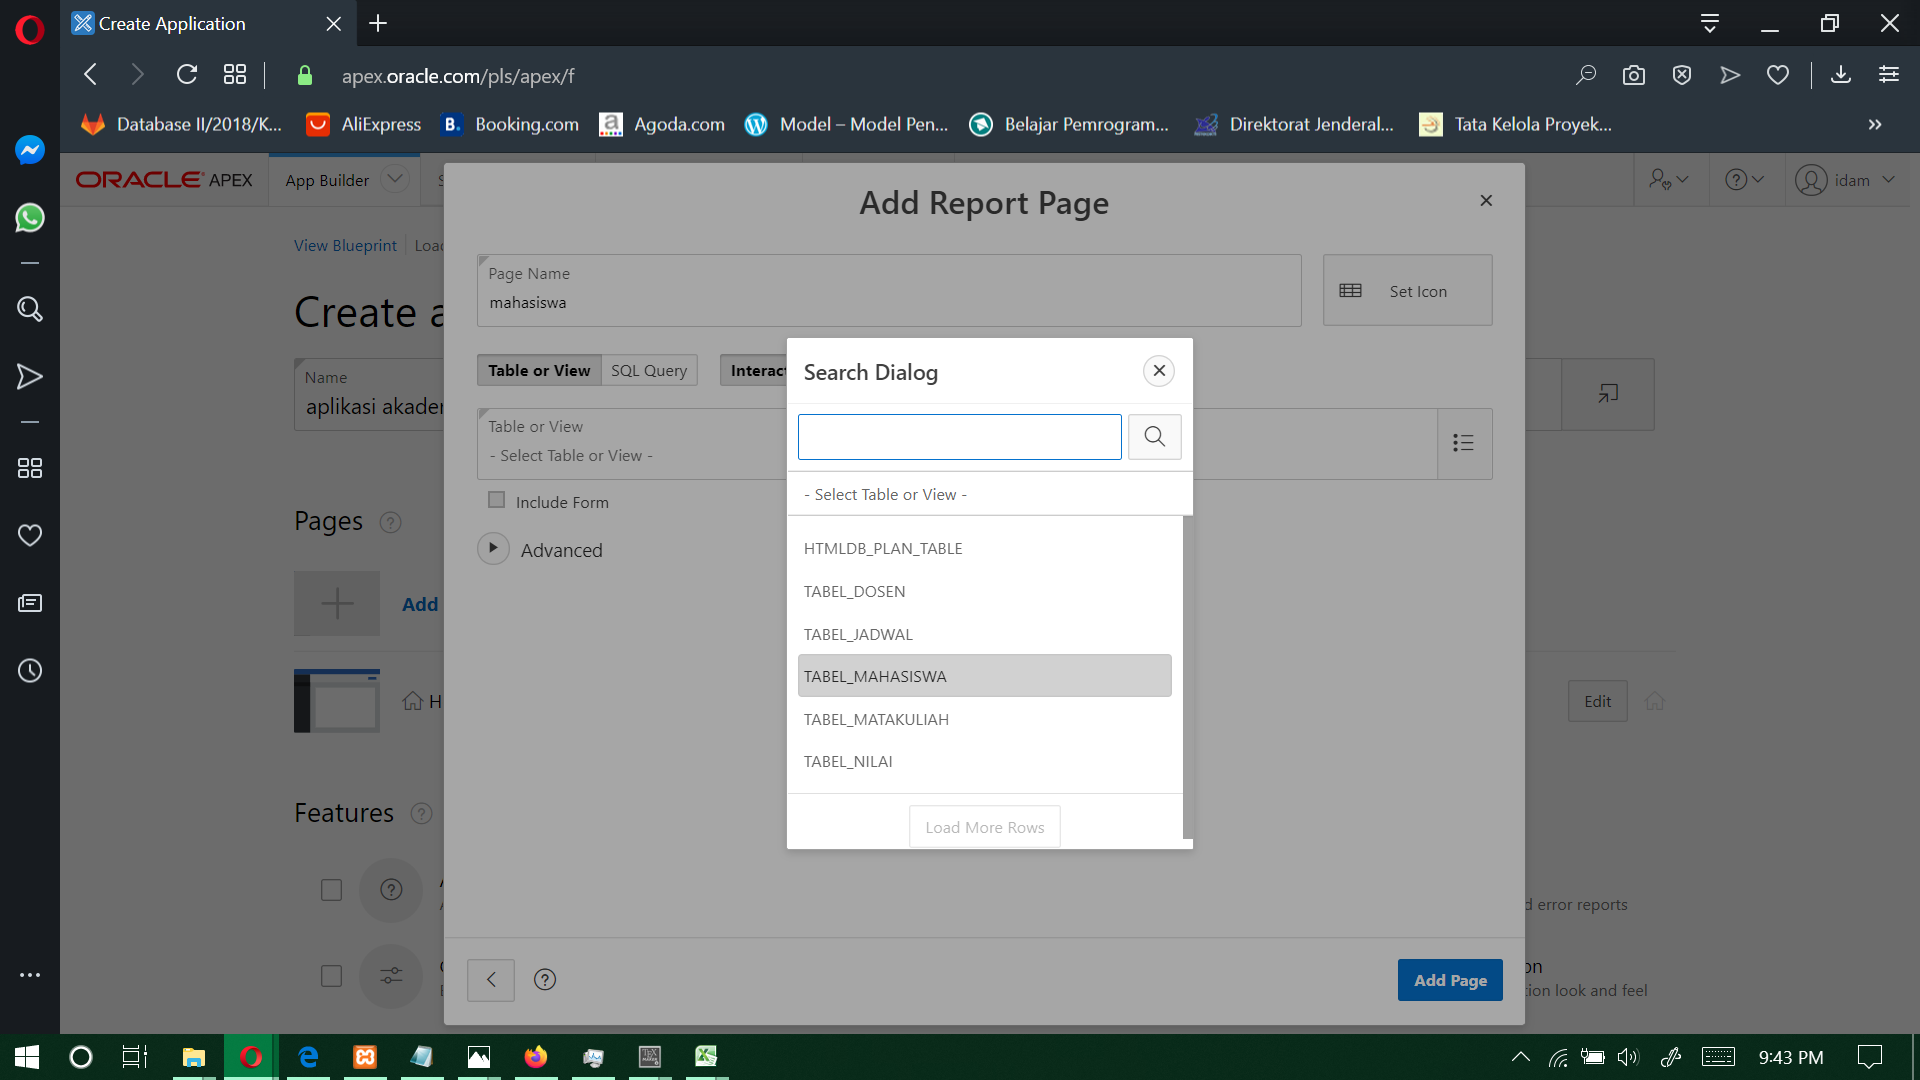
\includegraphics[width=10cm]{figures/add page/Screenshot (238).png}
    \caption{\textit{memilih tabel yang akan digunakan}}
    \label{foto21}
 	\end{figure}
	\item jika sudah maka klik "Add Page"
	\begin{figure}[H]
    \centering
	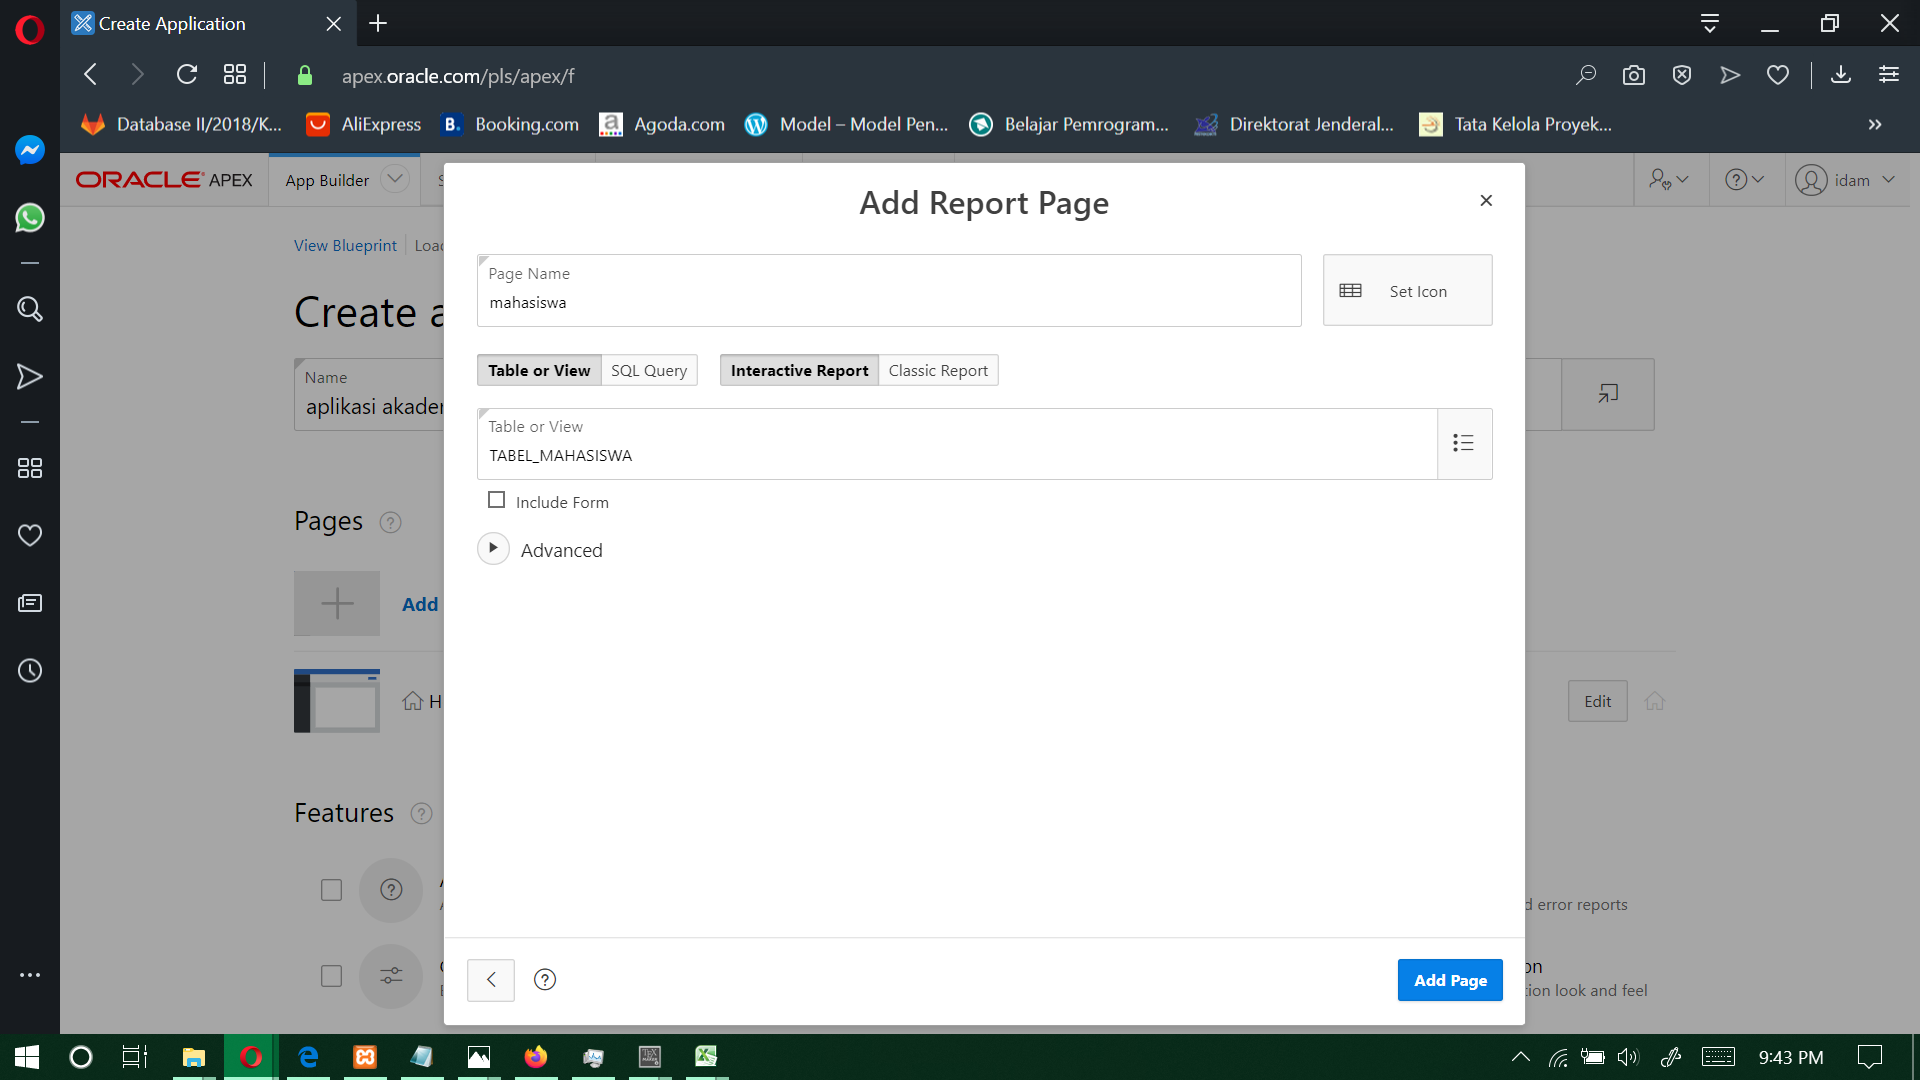
\includegraphics[width=10cm]{figures/add page/Screenshot (239).png} 
    \caption{\textit{menambahkan page pada aplikasi}}
    \label{foto21}
 	\end{figure}
	\item ulangi langkah diatas dengan memasukan tabel mahasiswa, dosen, dan matakuliah
\end{enumerate}
\subsection{menambahkan page dari tabel nilai dan jadwal dengan sql query}
\paragraph{}
pada kedua page ini kita akan mengambil data dengan menggunakan sql \textit{query}, caranya sebagai berikut :
\begin{enumerate}
	\item hampir sama seperti sebelumnya, klik "Add Page", pilih "interactive report"
	\begin{figure}[H]
    \centering
	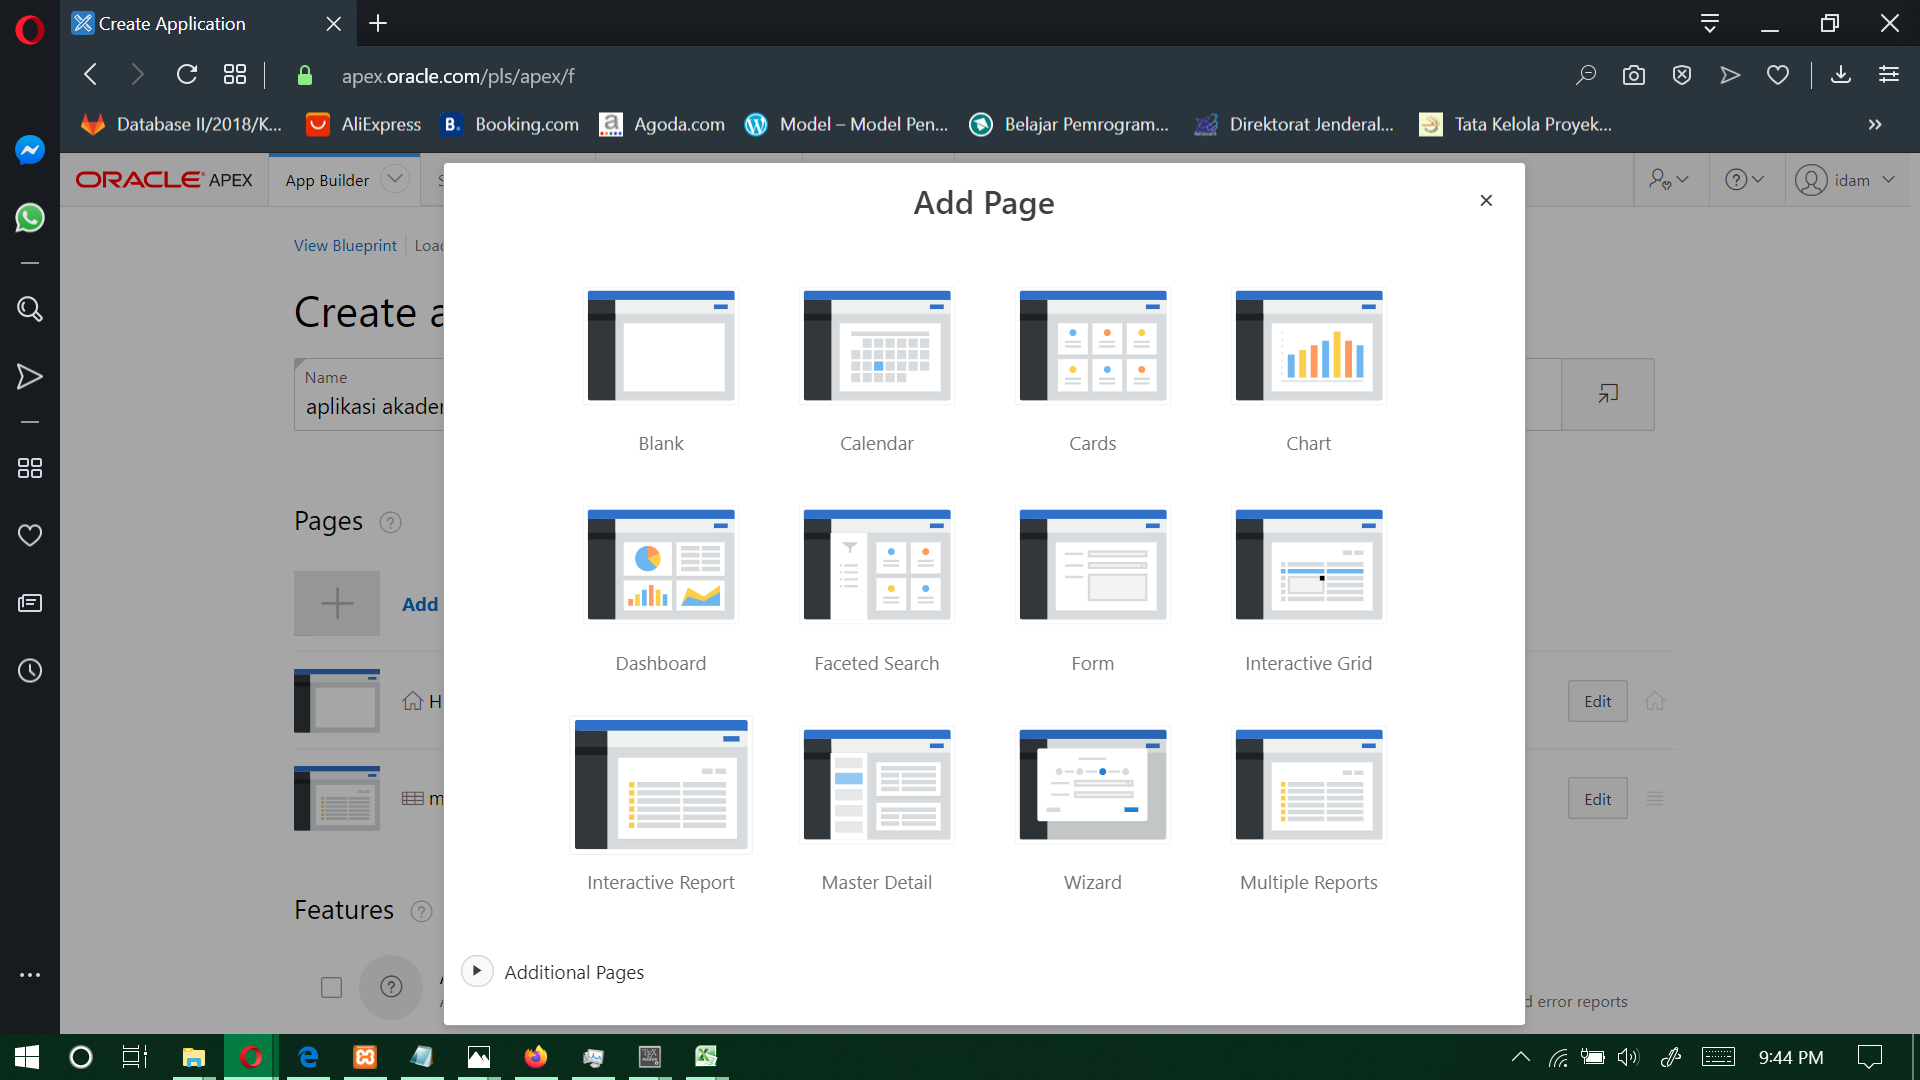
\includegraphics[width=10cm]{figures/add page/Screenshot (241).png} 
    \caption{\textit{menambahkan page pada aplikasi}}
    \label{foto21}
 	\end{figure}
	\item isi "Page Name" dengan nama "jadwal" lalu klik "SQL Query", kemudian ketikan \textit{query} sql, sebagai berikut :
	\begin{verbatim}
	SELECT tabel_matakuliah.nama_matakuliah, tabel_dosen.nama_dosen, 
	tabel_jadwal.waktu, tabel_jadwal.tempat
	FROM tabel_jadwal
	INNER JOIN tabel_matakuliah 
	ON tabel_jadwal.kode_matakuliah=tabel_matakuliah.kode_matakuliah
	INNER JOIN tabel_dosen 
	ON tabel_jadwal.kode_dosen=tabel_dosen.kode_dosen
	\end{verbatim}
	\begin{figure}[H]
    \centering
	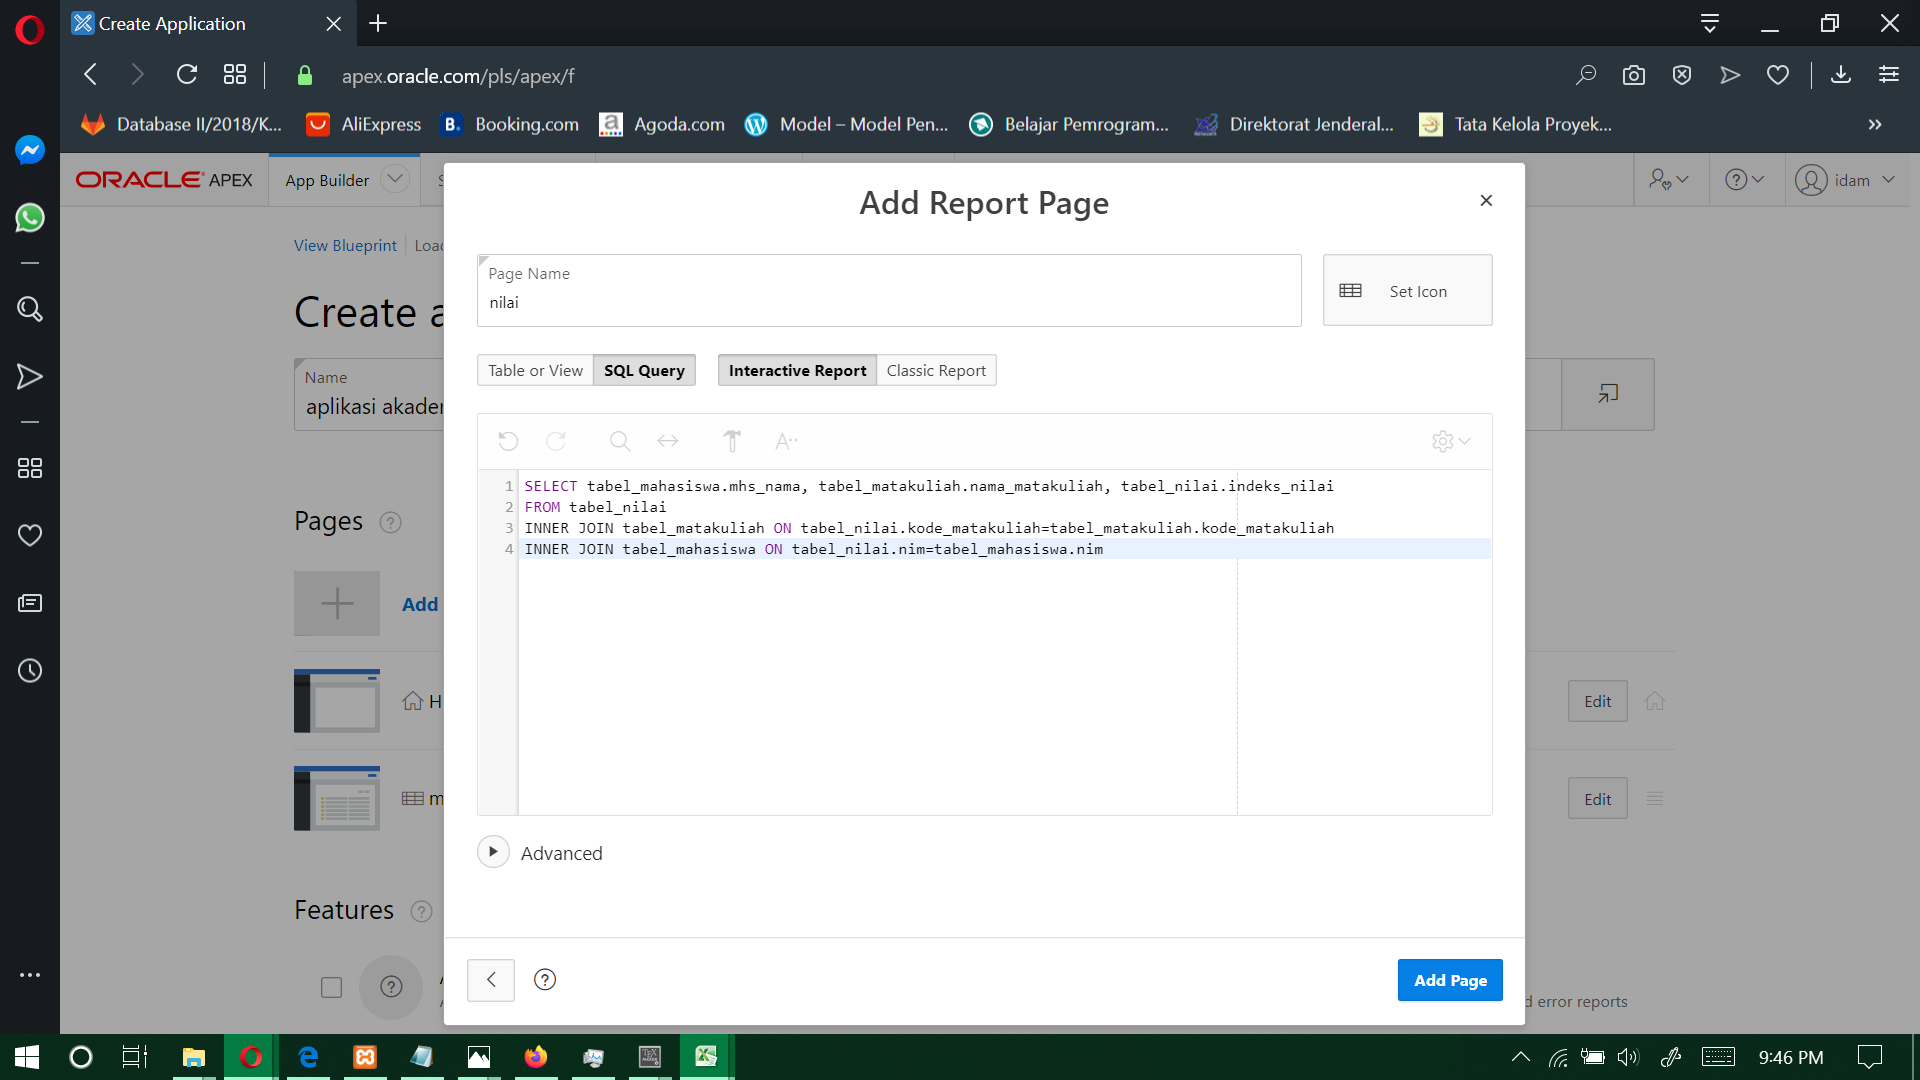
\includegraphics[width=10cm]{figures/add page/Screenshot (243).png} 
    \caption{\textit{menambahkan page dengan data dari query sql}}
    \label{foto21}
 	\end{figure}
	\item jika sudah maka klik "Add Page"
	\item  klik "Add Page" untuk menambahkan page "nilai"
	\item isi "Page Name" dengan nama "nilai" lalu klik "SQL Query", kemudian ketikan \textit{query} sql, sebagai berikut :
	\begin{verbatim}
	SELECT tabel_matakuliah.nama_matakuliah, 
	tabel_dosen.nama_dosen, tabel_jadwal.waktu, tabel_jadwal.tempat
	FROM tabel_jadwal
	INNER JOIN tabel_matakuliah 
	ON tabel_jadwal.kode_matakuliah=tabel_matakuliah.kode_matakuliah
	INNER JOIN tabel_dosen 
	ON tabel_jadwal.kode_dosen=tabel_dosen.kode_dosen
	\end{verbatim}
	\begin{figure}[H]
    \centering
	 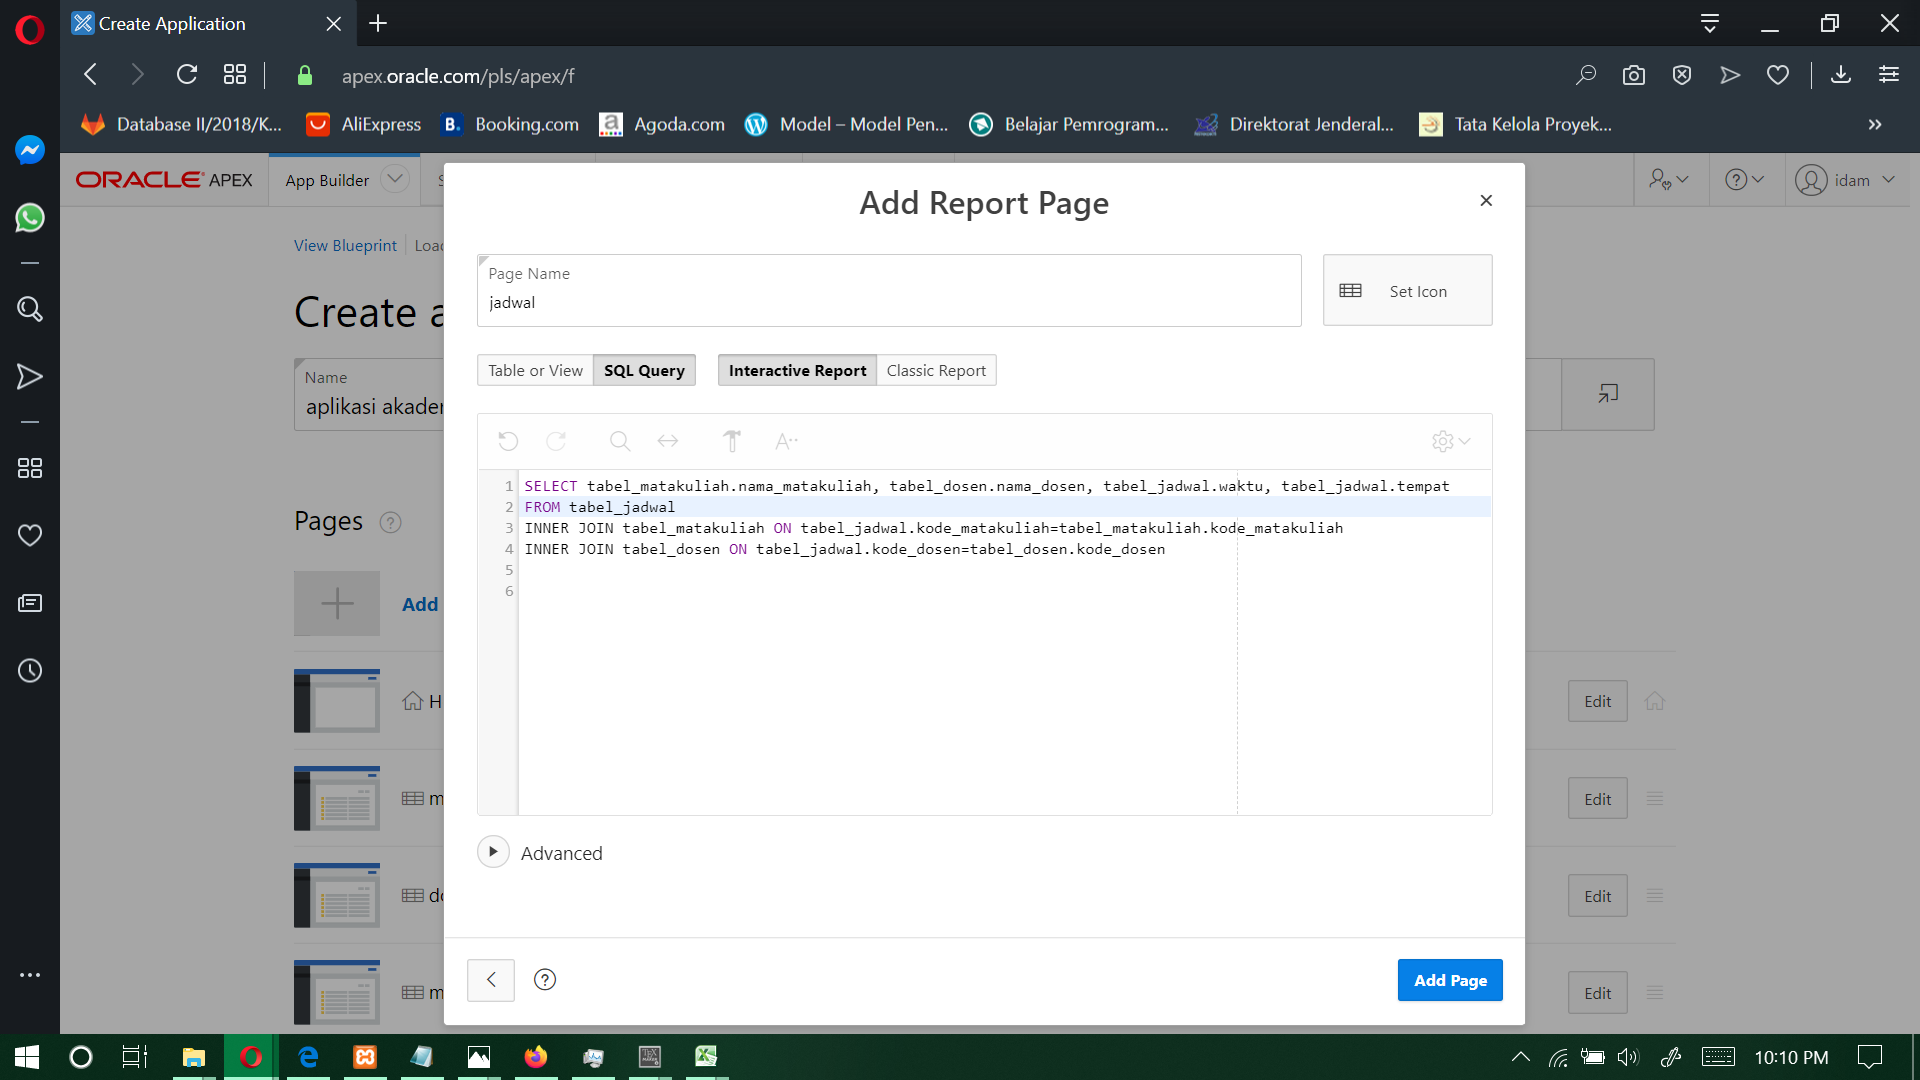
\includegraphics[width=10cm]{figures/add page/Screenshot (246).png} 
    \caption{\textit{menambahkan page dengan data dari query sql}}
    \label{foto21}
 	\end{figure}
	\item jika sudah maka klik "Add Page"
\end{enumerate}
\section{menjalankan aplikasi websheet}
jika semua page telah dibuat maka langkah selanjutnya, sekarang tinggal mencoba menjalankan aplikasi websheet yang kita buat, caranya sebagai berikut :
\begin{enumerate}
	\item sebelum menjalankan aplikasi, klik "Create Application" terlebih dahulu.
	\begin{figure}[H]
    \centering
	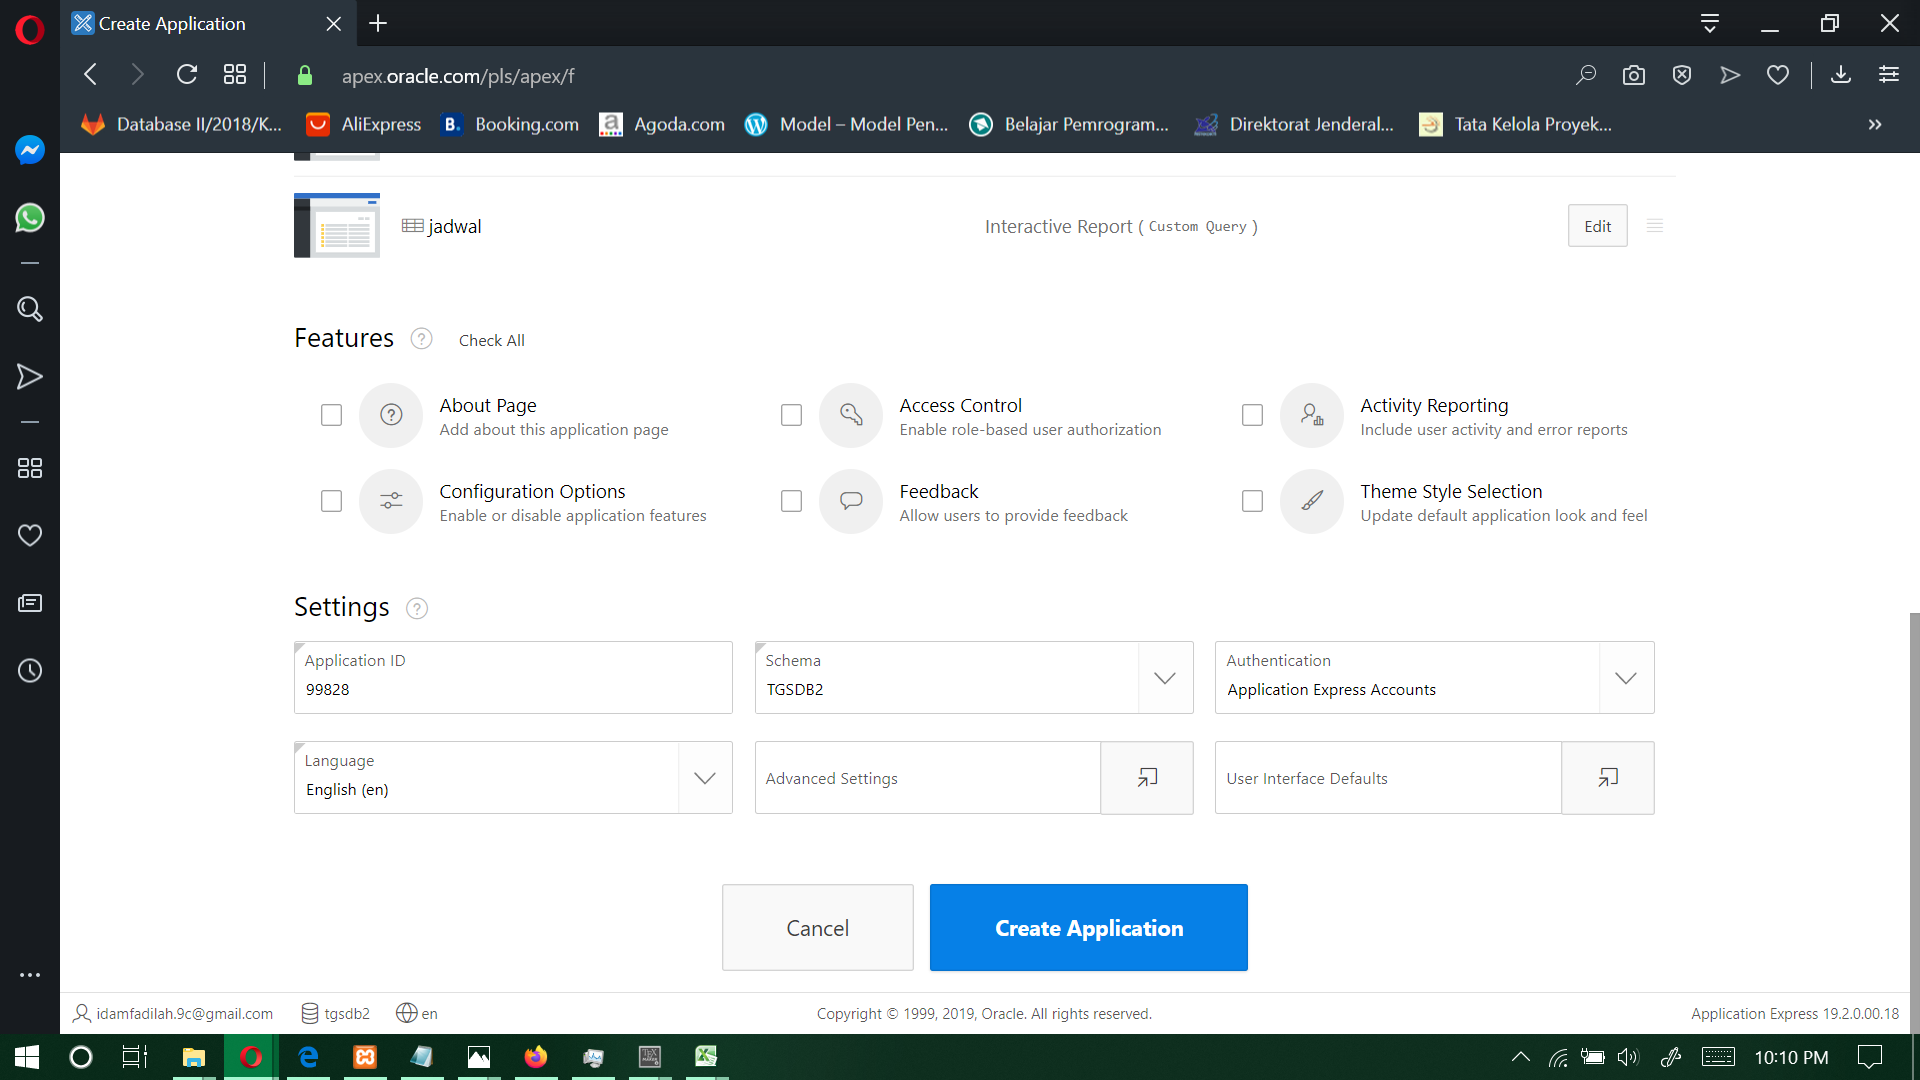
\includegraphics[width=10cm]{figures/run app/Screenshot (247).png} 
    \caption{\textit{oracle apex - app builder}}
    \label{foto21}
 	\end{figure}
	\item setelah itu klik "Run Application".
	\begin{figure}[H]
    \centering
	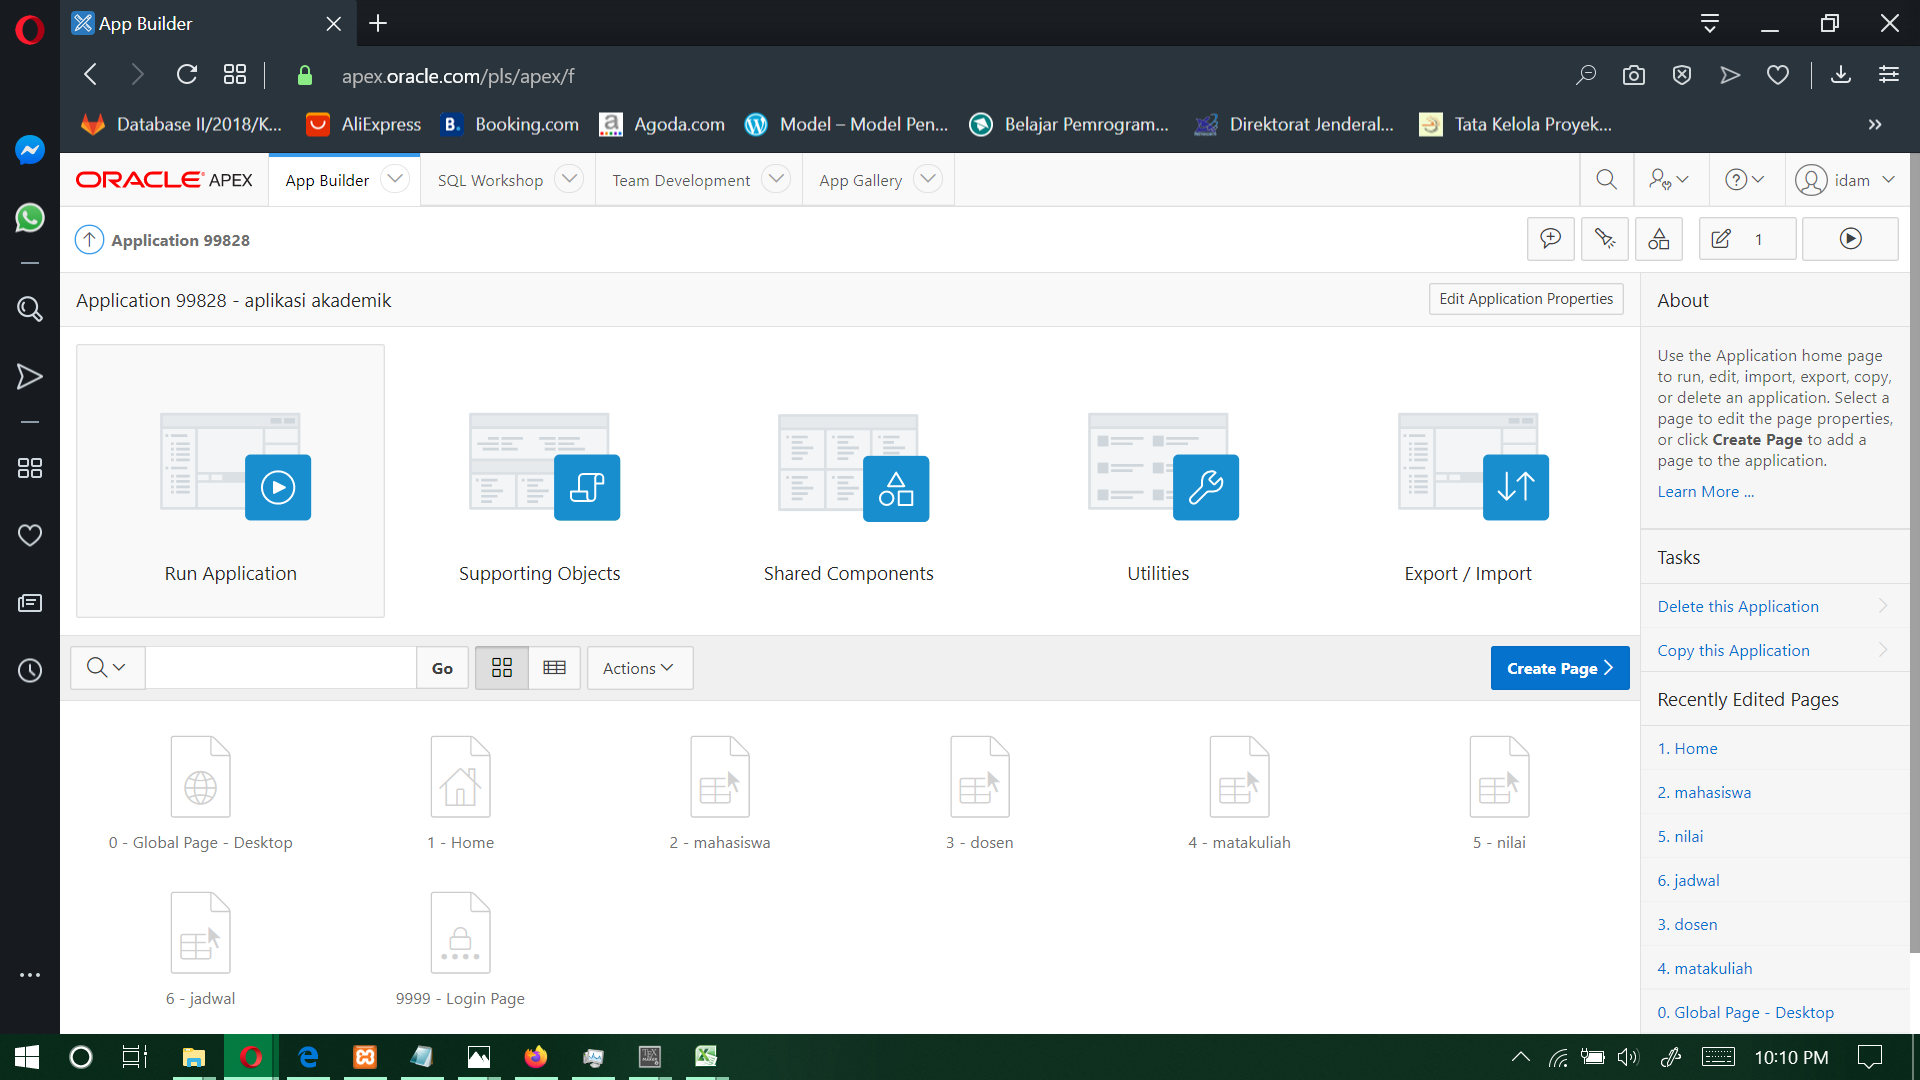
\includegraphics[width=10cm]{figures/run app/Screenshot (248).png} 
    \caption{\textit{menu konfigurasi aplikasi}}
    \label{foto21}
 	\end{figure}
	\item Login menggunakan username dan password apex.
	\begin{figure}[H]
    \centering
	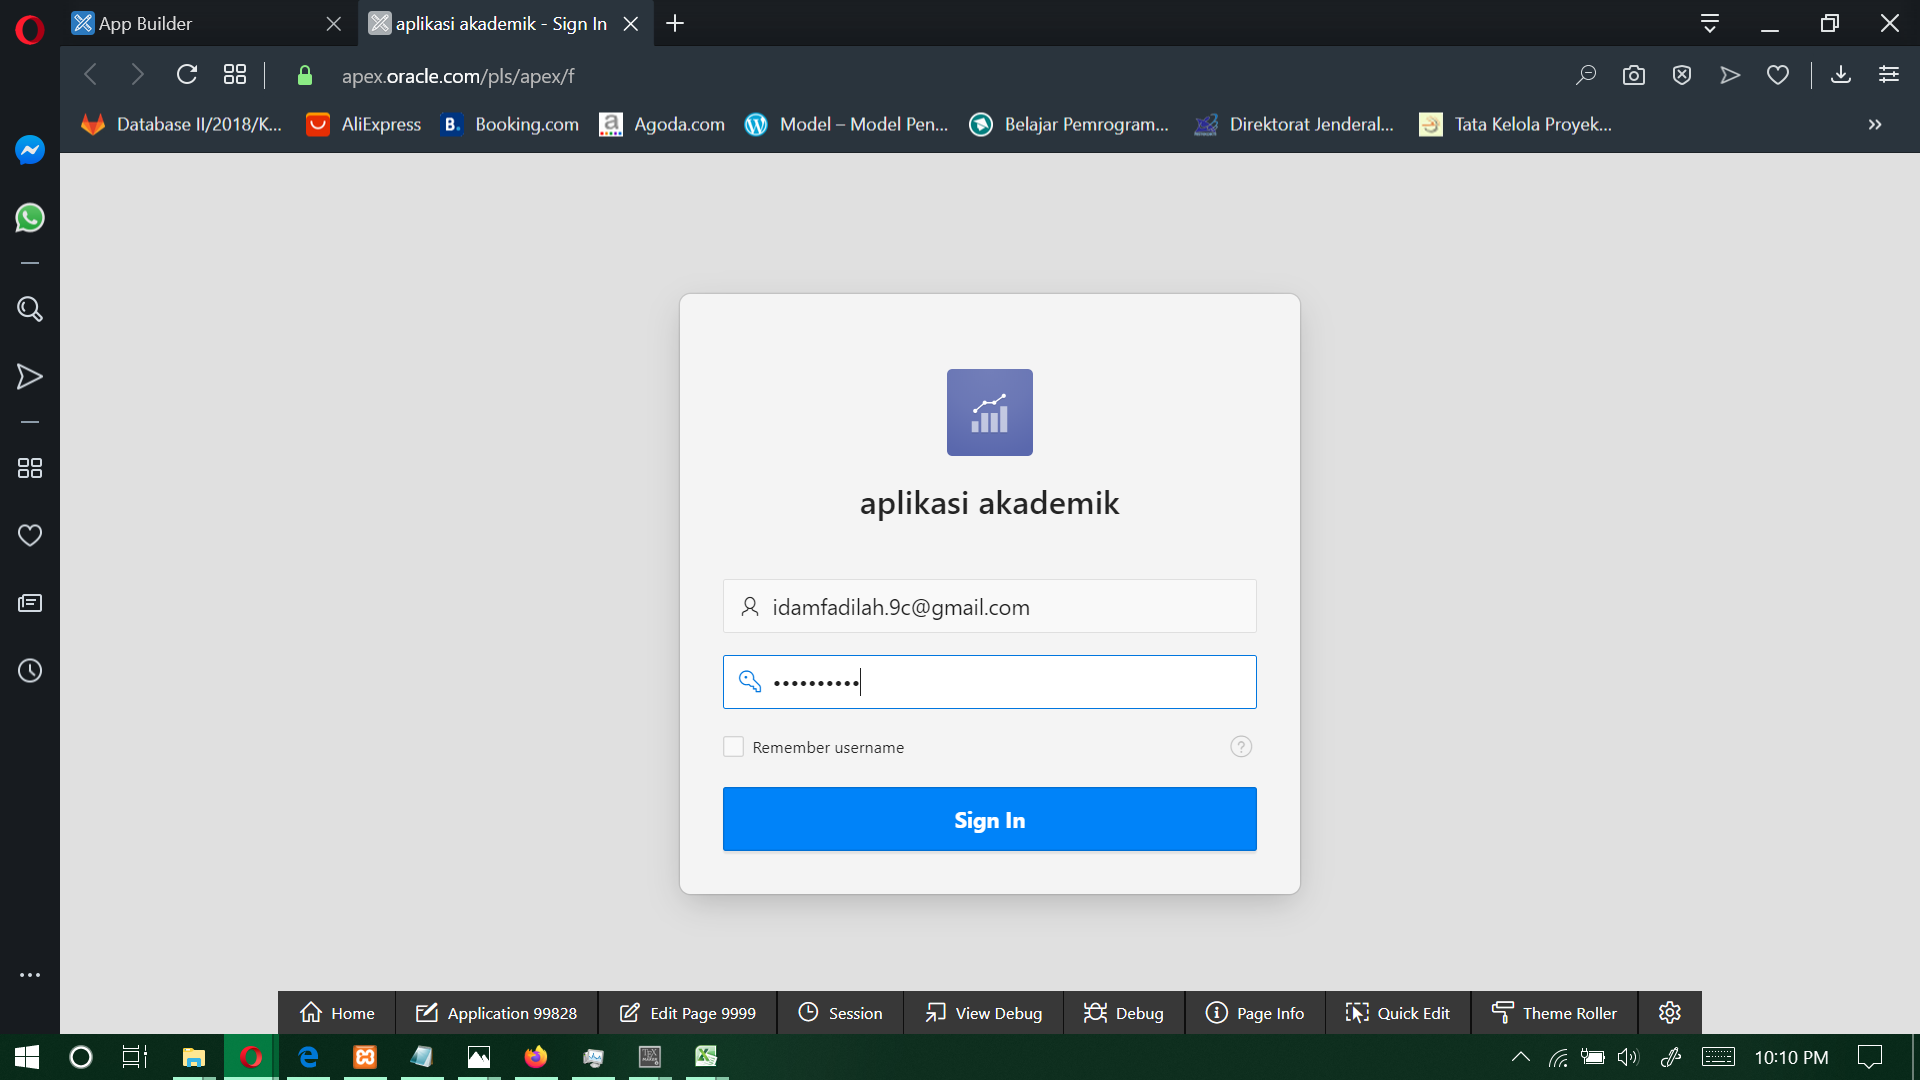
\includegraphics[width=10cm]{figures/run app/Screenshot (249).png} 
    \caption{\textit{login aplikasi}}
    \label{foto21}
 	\end{figure}
	\item dan inilah hasil aplikasi yang telah kita buat tadi. 
	\begin{figure}[H]
    \centering
	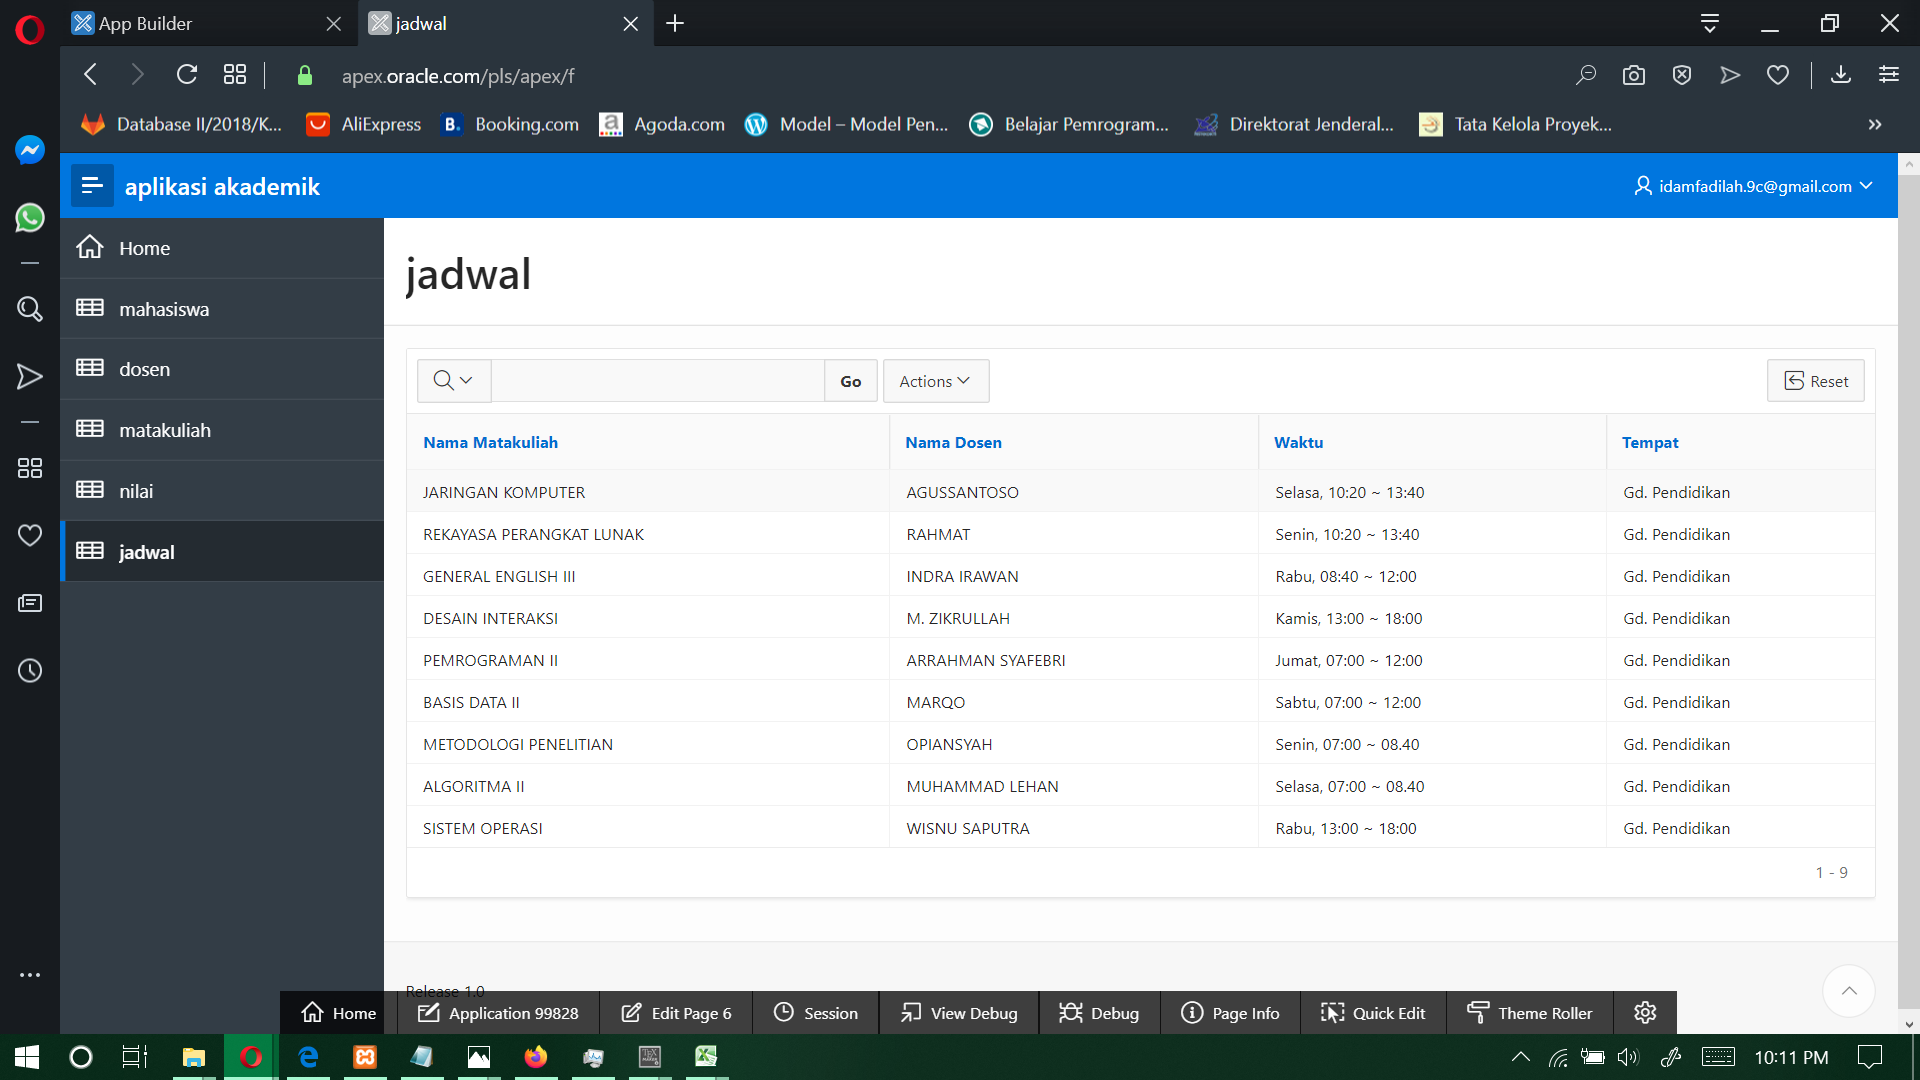
\includegraphics[width=10cm]{figures/run app/Screenshot (250).png} 
    \caption{\textit{tampilan aplikasi}}
    \label{foto21}
 	\end{figure}
\end{enumerate}
link aplikasi : \url{https://apex.oracle.com/pls/apex/f?p=99828:6:1984675557292::NO:::}\\
username 	  : idamfadilah.9c@gmail.com\\
password      : jcj223vi35\\
\end{document}
